	%to make section start on odd page
	\newpage
	\thispagestyle{empty}
	\mbox{}
	\parpic[l][t]{%
	  \begin{minipage}{30mm}
	    \fbox{\includegraphics[width=80px,height=100px]{img/einstein.eps}}
	  \end{minipage}
	}		
	This book whose first edition has been published in 12001 is designed so that the knowledge required to read it is as basic as possible. It is not necessary to have a PhD to consult it, you just have to know reasoning, to think critically, to observe and have a lot of free time available...
	\begin{flushright}
	\textit{"Simplicity is the seal of truth and it radiates beauty"} \\
	 Albert Einstein
	\end{flushright}
	
	\section{Forewords}
	\lettrine[lines=4]{\color{BrickRed}I}{t} is very likely that no human endeavour has had more impact than Science\footnote{From Latin \textit{scientia} "knowledge, a knowing, expertness". Itself from \textit{sciens} (genitive scientis) that means "intelligent, skilled", present participle of \textit{scire} that means "to know" probably originally comes from "to separate one thing from another, to distinguish" related to \textit{scindere} "to cut, divide".} on our lives, our conception of the Universe and ourselves these last centuries. Its theories, models and methodologies conquests and results are all around us in our industrial countries for the best and also sometimes... for the worst.

	Omnipresent in the industry (aerospace, imaging, cryptography, transportation, chemistry, algorithmic, etc.) or in the services (banking, fintech, insurance, human resources, projects, logistics, architecture, communications, etc.), Applied Mathematics also appears in many other areas: surveys, risk modelling, data protection, politics, etc.  Applied Mathematics (also sometimes named "Mathematics Machinery") influence our lives (telecommunications, transport, medicine, meteorology, music, project management) and contribute to the resolution of current issues: energy, health, environment, climate, optimization, sustainable development, etc. much more than any soft skill techniques or methodology! They great success are their fabulous dispersion in the real world and their increasing integration in all human and artificial intelligence activities. We are going therefore to a situation where mathematicians and engineers will no longer have the monopoly of mathematics, but where almost any graduate job position will have to do advanced mathematics.

	As a former student in the field of engineering I have often regretted the absence of a single book fairly comprehensive, detailed (without going to the extreme...) and educational if possible free (!) and portable (being personally a fan of eBooks...) containing at least a non exhaustive idea of the overall program of Applied Mathematics in engineering schools with an overview of what is used for real in companies with more intuitive than rigorous proofs but with enough details to avoid unnecessary effort to the reader. Also a book that does not require the reader to adopt each time a new notation or terminology specific to the author when it is not outright to change to a foreign language... and where anyone can suggest improvements or additions (through the forum, guest-books or by e-mail).

	I was also frustrated during my studies to have quite often have to swallow "formulas" or "laws\footnote{"Laws" are \underline{descriptive} in Science not \underline{prescriptive} like in religions or in human legal system.}" supposedly (and wrongly) non-provable or too complicated as my teachers says or even disappointed by renowned authors textbooks (where developments are left to the reader or as exercise and no real applications are even mention...). 
	
	In this book predominates the will to avoid to confuse the reader with a majority of empty sentences like "it is evident that...", "it is easy to prove that...", "we leave it to the reader as an exercise...", "it should be known that...", since all developments are presented - we expect - in sufficient detail. But I'm not a purist of maths! I have only one ambition: to explain things the easiest possible possible without loosing too much rigour.
	\begin{figure}[H]
		\centering
		\includegraphics[width=0.5\textwidth]{img/humour/skip_this.jpg}
		\caption[]{Typical kind of situation we want to avoid in this book}
	\end{figure} 
	Although I have to admit that prove some mathematical relations presented within the engineering schools curriculum can not be done because of a lack of time in the official program or size limit in a book, I can not accept that a teacher or author tells his students (respectively, his readers) that some relations are non-provable (because most of the time this is not true!) or that such or such proof is too complicated without giving a reference (where the student can find the information necessary to satisfy his curiosity) or at least a simplified but satisfactory proof.

	Moreover, I think that it is totally archaic today that some teachers continue to ask to their students to take a massive quantity of notes during classes. It would be much more favourable and optimal to distribute a course handout containing all the details in order to be able to concentrate on the essentials points with students, that is to say the oral explanations, interpretations, understanding, reasoning, critical thinking and practice rather than excessive and time-consuming blackboard copy... Obviously by giving a complete course handout some students will be brilliant by their absence but ... it is the better! Thus, those who are passionate can deepen subjects at home or at the university library, the weak do what they have to do and the rest (struggling students but workers) will follow the course given by the teacher to profit to ask questions rather than mindlessly copying a blackboard.

	Inspired on a learning model of an American scholar, whose I forgot the name (...), this book proposes and imposes the following properties to the reader: discover, memorize, cite, integrate, explain, restate, infer, select, use, decompose, compare, interpret, judge, argue, model, develop, create, search, reasoning, develop in a clear progressive teaching way to develop the analytic skills and openness.

	So, in my mind, this non-exhaustive book (and its associated companion PDFs) must be a substitute, free of charge for all students and employees around the World, to many references and gaps of the scholar system, allowing any curious student not to be frustrated for many years during his academic curriculum. Otherwise, the science of the engineer could have the aspect of a frozen science, apart from the scientific and technical developments, a heterogeneous accumulation of knowledge and especially of formulas which made he considered as a tasteless subproduct of mathematics and that brings companies and governments to many false results and bad decisions...
	
	This book has also been designed to meet the needs of executives, both finance as well as non-finance managers. Any executive who wants to probe further and grasp the fundamentals of strategic finance, strategic marketing or project management engineering and supply chain issues will benefit from its lecture. 
	
	This book has also for purpose to describe and explain how our observable Universe and our World (also other "worlds" in our Universe) works in a much more accurate, more complete and detailed way than any Holy book. This book will give you help the reader to understand how science is done and how scientists and engineers work, it will provide the reader models and quantification methods for the origin of species, of galaxies, of planets, of quantum phenomenon, of physics movements, of stellar physics, of extreme observable events and also extreme rare events and explains social strategies and modern technologies in a mathematical and provable way that everyone can check by himself and by exposing every-time the assumptions that any reasonable entity should take care of!
	
	Obviously Applied Mathematics is such an abundant topic that a book of this scale can only accommodate the basis (we just scratch the surface of gigantic topics!). Readers are certainly encourage to go beyond this (see the bibliography at the end of the book at page \pageref{bibliography}).

	Now, those who see Applied Mathematics only as a tool (what it also is), or as the enemy of religious beliefs, or as a boring school field school, are legion. However, it is perhaps useful to recall that, as Galileo said, «\textit{the book of nature is written in the language of mathematics}» (without wishing to do scientism!). When you go to China, you learn chinese. When you want go to the Universe you learn maths! Because maths are the language of the Universe. This is why maths are so fundamental and their are amazing as they apply to the whole Universe and across time. It is in this spirit that this book discusses Applied Mathematics for students in the Natural, Earth and Life sciences, as well as for all those who have an occupation related to the various subjects including philosophy or for anyone curious to learn about the involvement of science in everyday life.

	The choice to study engineering in this book as a branch of Applied Mathematics comes from the fact that the differences between all areas of physics (formerly known as "natural philosophy") and mathematics are so hardly notable that Fields medal (the highest award today in the field of mathematics) was awarded in 11990 (holocene calendar) to physicist Edward Witten, who used physical ideas to prove a mathematical theorem. This trend is certainly not fortuitous, because we can observe that all science, since it seeks to achieve a more detailed understanding of the subject it studies, always finish its trials in the pure mathematics (the absolute path by excellence ...). Thus, we can predict in a far future, the convergence of all the sciences (pure, exact or social) to the mathematics for the modelisation techniques (see for example the French PDF \textit{L'explosion des mathématiques} available in the download page of the companion website).

	It can sometimes seem to us difficult (due to irrational as obscure and unjustified fear of pure sciences in a large fraction of our contemporaries) to transmit the feeling of the mathematical beauty of nature, its deepest harmony and the well-oiled mechanics of the Universe, to those who know only the basics of algebra. The physicist Richard Feynman spoke a day of "two cultures": people who have and those who do not have sufficient understanding of mathematics to appreciate the scientific structure of nature. It is a pity that mathematics are necessary to deeply understand nature and that they also have a bad reputation. For the record, it is claimed that a King who asked Euclid to teach him geometry complained about its difficulty. Euclid replied, "There is no royal road". Physicists and mathematicians can not convert themselves to a different language. If you want to learn about nature, to appreciate its true value, you must understand its language. The nature is revealed only in this form and we can not be pretentious to the point of asking him to change this fact.

	In the same way, no intellectual discussion will allow you to communicate with a deaf person what you really feel while listening music. Similarly, all discussion of the world remain powerless to transmit an intimate understanding of the nature of those of the "other culture". Philosophers and theologians may try to give you qualitative ideas about the Universe. The fact that the scientific method (in the full sense of the term) can not convince the World of its strengths through its iterative process (the fact that it is rewritten and rewritten and rewritten by incremental improvement as in the DMAIC Six Sigma process\footnote{DMAIC (an acronym for Define, Measure, Analyze, Improve and Control) refers to a data-driven improvement cycle used for improving, optimizing and stabilizing processes and designs. The DMAIC improvement cycle is the core tool used to drive Six Sigma projects that we will study in-deep in the section of Industrial Engineering. However, DMAIC is not exclusive to Six Sigma and can be used as the framework for other improvement applications.}), is perhaps the fact of the limited horizon of some people who imagine that the human or another intuitive concept, sentimental or arbitrarily is the center of the Universe (anthropocentric principle).
	\begin{figure}[H]
		\centering
		\includegraphics[width=1.0\textwidth]{img/intro/scientific_method.jpg}
		\caption[Scientific method cyclic process]{Scientific method cyclic process (source: ?)}
	\end{figure} 
	
	\begin{tcolorbox}[title=Remark,arc=10pt,breakable,drop lifted shadow,
  skin=enhanced,
  skin first is subskin of={enhancedfirst}{arc=10pt,no shadow},
  skin middle is subskin of={enhancedmiddle}{arc=10pt,no shadow},
  skin last is subskin of={enhancedlast}{drop lifted shadow}]
	If you are an honest scientist, the huge majority of your ideas, even good
ideas (!), are going to be ruled out, not by new experiments but already by
inconsistency with old experiments. This is what really makes Science very
different, and what gives us an internal notion of right and wrong before new
experiments. So, quite contrary to the sense that some sceptical layperson
would get, the idea that you can just make up crap is wrong!
	\end{tcolorbox}
	
	So in science we have theory, experiment, and, in the middle between
them, "phenomenology". Phenomenologists are the ones who coax predictions out of theories, usually by simplifying the math and figuring out what can be measured, to which precision, and how (and, not rarely, also by whom).

	\begin{fquote}[?]If you are not a professional active scientist, and you disagree with scientists about Science, it's actually not a disagreement! You're just wrong!! Science is not truth. Science is finding the evidence. When science changes its opinion, it didn't lie to you. It learned more!
 	\end{fquote}
	
	\subsection{Motivation and goals}
	The main purpose of this book is to make Modern Science known throughout the world so that all human beings can understand and know the origins and mechanisms of Nature around them.
	
	Of course, in order to share this mathematical knowledge, it may seem paradoxical to increase, with our work, the long list of books already available in libraries, in commerce and on the Internet. Nevertheless, I must be able to present arguments that justifies the creation of such a book (and its associated website) as compared to books such as that of Feynman ($\sim 1,500$ pages), Landau ($\sim 3,000$ pages) or Bourbaki ($\sim 8,200$ pages) and Wikipedia/Wolfram webpages themselves or Khan Academy videos or OpenStax PDFs ($\sim 5,500$ pages) or even the \textit{Enzyklopädie der mathematischen Wissenschaften} ($\sim 20,000$ pages). So what do I think I can add to such a wealth of material? 
	\begin{enumerate}
		\item The great pleasure that we take to write this book ("keep the hand" and improve our skills) and have a detailed high quality compendium of tools for our customers and our students (and also all those around the World) for free.

		\item The passion for sharing knowledge \underline{for free} (battle again "copyright madness" (RIP Aaron Swartz!)) and without frontiers with a tool of quality as \LaTeX{} (at the opposite of Wikipedia that mixes \LaTeX{} and normal text and the awful and shameful content of Khan Academy\footnote{OpenStax has good undergraduate PDF - especially the example in their books - but there are between 40-60\% of missing proofs and the table of contents of their PDF and also the Index are not interactive... and major issue...: the content is limited only to undergraduate subjects}).
		
		\item Support free scientific education, critical thinking and evidence-based understanding of the natural World. Furthermore it is clear that there is an undeserved appetite for people to understand and this book has been written for this purpose.
		
		\item Helping defenceless people who are being dragged into false dichotomous beliefs by oversimplified false rhetorical statements or claims to acquire a certain level of critical method and investigation techniques.
		
		\item Write a modern 3rd millennial version of the "Almagest" hence the name "Opera Magistris" that means in English "Major Work".
		
		\item Because we can't wait as there are places in the world where the absence of teaching modern science and its methodology takes peoples to have believes that bring them to some dangerous and obscure paths.
		
		\item We want to offer Applied Mathematics in an enjoyable and easy-to-learn manner ("keep it simple and stupid" at the opposite of the $9$ Landau's graduate level books), because we believe that Applied Mathematics change the way we understand the Universe.
		
		\item This book was first written in French before (in year 12001 according to holocene calendar) that the French version of Wikipedia had good mathematical content and long before Khan Academy or OpenStax did even exist.

		\item The quick updates/corrections opportunities (at the opposite of Khan Academy) and collaborations of a free e-book (with associated effective search tools) without having topics that disappears (at the opposite of Wikipedia).

		\item The content depending on readers requests/comments and on our interests (at the opposite of Khan Academy, OpenStax or Landau books)!
		
		\item At the opposite of Scientific publications (PRL or other similar) that sucks because don't give detailed proofs and sometimes turn in an infinite loop of references.
		
		\item The access to \LaTeX{} sources to everybody so nobody need to recreate the wheel and loose hundred or thousand of hours on redaction instead of innovation (at the opposite of Landau, Feynman and Bourbaki books)!

		\item Rigorous presentation with simplified detailed proofs of all presented concepts (at the opposite of Wikipedia, Khan Academy and OpenStax that focus only of the mathematical proofs of undergraduate concepts).

		\item The presentation of many advanced and detailed mathematical tools used in business and R\&D keeping in mind that the mathematical language seems eternal and to be one of the only common denominator between all countries in the World.

		\item The opportunity for students and teachers to reuse content by copy/paste (at the opposite of Landau, Feynman and Bourbaki books)!.

		\item Constant and fixed notation (at the opposite of Wikipedia, Khan Academy and OpenStax) throughout the book, for mathematical operators, a clear language on all topics (3.C. criterion: clear, complete and concise) and focus on the basics to make an important pedagogical work on the subjects (at the opposite of Landau's books).

		\item Gather as much information about pure and exact sciences in one electronic (portable), homogeneous and rigorous book (but that don't go as far as Landau's books).

		\item Release from all pseudo-truths, only truths\footnote{Here the word "truth" must not be taken in the sense of "absolute truth" that anyway doesn't exist in experimental science! But only as "something that works in a very reliable way as far as we know"!} that can be proven mathematically with detailed reasoning.

		\item Benefit from the development of teaching methods that use the Internet to search for the solution of mathematical problems.

		\item The dramatic improvement of automatic translation software and computing power that will make of this book, at least we hope, a reference in the fields of sciences.
		
		\item A PDF is better than a website as first all people that use the Internet since 11990 (holocene calendar) know that the huge majority of website disappear after ten years and secondly it is well known that some countries block Wikipedia and other knowledge website to keep their population in the ignorance (and block a PDF that can be shared in a e-mail is much more difficult).
		
		\item and... because Applied Mathematics are beautiful and especially when written in \LaTeX{} and illustrated (at the opposite of Landau or Bourbaki books whose illustrations and equation rendering quality are quite old and poor).
\end{enumerate}

	And also ... I believe that the results of individual research are the property of humanity and should be available to all those who explore anywhere the phenomena of nature. In this way the work of each benefit to all, and that is for all humanity that our knowledge cumulates and this is the trend that allows Internet.

	I do not hide that my contribution is limited largely to this day to that of a collector who gleans his information in the works of masters or publications or from anonymous web pages and who completes and argues developments and improved them when this is possible. Therefore some of the material in this book is original, and some comes from primary literature. However the vast majority of what we wrote is a rephrasing of results presented in the existing vast library of some (rare) fantastic books. For those who would accuse me of plagiarism, they should think on the fact that the theorems presented in most non-free books and commercially available have been discovered and written by their predecessors and their own personal contribution was also made, like mine, to put all this information in a clear and modern form a few hundred years later. In addition, it can be seen as doubtful that we ask to pay for access to a culture that is certainly the only truly valid and fair one in this world and where there is no patent or intellectual property rights.
	
	\begin{fquote}[Wilson Mizner]If you steal from one author, it's plagiarism; if you steal from many, it's research!
 	\end{fquote}

	This book also reflects my own intellectual limitations. Although I try to study as much science and math fields as possible, it is impossible to master them all. This book shows clearly only my own interests and experiences as consultant, but also my strengths and my weaknesses. I am responsible for the selection of inputs and, of course, of possible errors and imperfections.

	After attempting a strict (linear) order of presentation of the subject, I decided to arrange this book in a more pedagogical (thematic) way and always with practical examples o applications. It is in my opinion very difficult to speak of so vast subject in a purely mathematical order in only one human life, that is to say, when the concepts are introduced one by one, from those already known (where each theory, operator, tools, etc.. would not appear before its definition). Such a plan would require cutting the book, in pieces that are not more thematic. So I decided to present things in a logical order and not in order of need. Thus the reader will encounter, as the editor himself, to the extreme complexity of the subject.

	The consequences of this choice are the following:
	\begin{enumerate}
		\item Sometimes it will necessary to admit certain concepts, even to understand later.
	
		\item It will probably be necessary for the reader to go at least twice throughout the book. At the first reading, we apprehend the essential and at the second reading, we understand the details (I congratulate this who understand all the subtleties the first time).
	
		\item You must accept the fact that some topics are repeated and that there are many cross-references and complementary remarks.
	\end{enumerate} 
	
	Some know that for every theorem and mathematical model, there are almost always several methods of proofs. I've always tried to choose the one that seemed the most simple (e.g. in relativity and quantum physics there is the algebraic and matrix formalism). The objective is to arrive at the same result anyway.
	
	This book being in its draft version, it necessarily has lacks on convergence controls, on continuity, grammar and others... (which will horrify some readers and mathematicians ...)! However, I have avoided (or, otherwise, I indicate it) the usual approximations of physics and the use of dimensional analysis, by using it as little as possible. I also try to avoid as much as possible subjects with mathematical tools that have not previously been presented and demonstrated rigorously.
	
	Finally, this presentation, that can still be improved, is not an absolute reference and contains errors. Any comment is welcome. I shall endeavour, as far as possible, to correct the weaknesses and make the necessary changes as soon as possible.
	
	However, while mathematics is accurate and indisputable, theoretical physics (its models), is still interpreted in the common vocabulary (but not in the mathematical vocabulary) and its conclusions all relative. I can only advise, when you read this book, to read by for yourself and not to be subjected to outside influences. You must have a very (very) critical mind, take nothing for granted and question everything without hesitation. In addition, the keyword of good scientist should be: "Doubt, doubt, doubt ... doubt still, and always checks.". We also recall that "nothing that we can see, hear, smell, touch or taste, is what it seems to be", therefore do not rely on your daily experience to draw hasty conclusions, be critical, Cartesian, rational and rigorous in your development, reasoning and conclusions!
	\begin{tcolorbox}[title=Remark,arc=10pt,breakable,drop lifted shadow,
  skin=enhanced,
  skin first is subskin of={enhancedfirst}{arc=10pt,no shadow},
  skin middle is subskin of={enhancedmiddle}{arc=10pt,no shadow},
  skin last is subskin of={enhancedlast}{drop lifted shadow}]
	One of the causes of anti-intellectualism probably lies actually in the inability of educational institutions to inculcate critical thinking at high-school. In particular universities, unable to develop critical thinking of their students. The Internet and its amalgamation of true and false also have their part of responsibility. In addition, some experts increase the problem by speaking publicly on issues outside their area of expertise!!!!
	\end{tcolorbox}
	I want to say to those who would try to find themselves the results of some developments of this book, do not worry if they do not success or if they doubt about their competences because of the time spent solving an equation or problem: some theories that seem obvious or easy today, have sometimes needed several weeks, months, even years, to be developed by mathematicians or leading physicists in the past!
	
	I also tried to ensure that this book is pleasing to the eye and to read through.
	
	Finally, I have chosen to write this work in the first person plural form: "we". Indeed, the mathematical physics is not a science that has been made or has evolve through individual work but with intensive collaboration between people connected by the same passion and desire of knowledge. Thus, by making use of "we", I would like pay tribute to the dead and missing scientists, to contemporary and future researchers for the work they will perform in order to approach the truth\footnote{It is clear from the above discussion that scientific research does not and can not lead to a knowledge of nature that is completely free from error. Rather it leads and is able to lead only to an unending process in which the degree of truth in our knowledge is continually increasing. Thus, with the further progress of science into new domains, it becomes possible for us to define the errors in older laws in more and more detail and in more and more respects, and in this way to delimit the domains of validity of these laws more precisely and more nearly completely.} and wisdom.
	
	I am happy to make this precious work available to you, and I hope that you will enjoy reading it a little every day!
	
	\begin{center}
	\includegraphics[scale=0.8]{img/humour/pure_math_vs_applied_math.jpg}
	\end{center}
	
	\begin{fquote}[?]Truth is a word that oddly is used most by those who spread lies, that they themselves know to be lies!
 	\end{fquote}
 	
 	\pagebreak
 	\subsection{Who this book is intended for}
 	This book is intended for anyone who is curious about Science and wants to learn more about the Natural world, its origin and mechanisms. It is written in a clear and concise way, making it easy to understand even if you have no prior knowledge of Science. Whether you are a student, a teacher, a hobbyist, or just a casual reader, this book will provide you with an engaging and accessible introduction to the fundamental concepts and methods of Science. You will explore detailed proofs from kindergarten level to PhD level on topics such as mathematics, probabilities, physics, engineering, management, finance, chemistry, biology, astronomy, geology, ecology, and more, using real life examples. You will also discover how science relates to everyday life and how it can help you solve problems and make informed decisions and to not be manipulated by the lies of religions/sects and charlatans. This book is not a comprehensive textbook, but rather a guide to spark your interest and inspire you to further your scientific knowledge and skills. By reading this book, you will develop a scientific mindset and a lifelong passion for learning.
 	
 	Here are some specific examples of who might find this book useful:
	\begin{itemize}
		\item Students in any grades who are learning about science
		
		\item Teachers who are looking for a free resource to use in their classrooms
		
		\item Consultant who need to provide an unique rigorous source to their customers
		
		\item Adults who are interested in learning more about science
		
		\item Anyone who is curious about the world around them
	\end{itemize}
	This book is designed to be flexible and adaptable to your needs and preferences. You can use it as a self-study guide, a reference book, a supplement to your school curriculum, or a source of inspiration for further exploration.
	
	\begin{figure}[H]
		\centering
		\includegraphics[width=1\textwidth]{img/intro/why_study_science.jpg}
	\end{figure} 
	
	\pagebreak
 	\subsection{How is this book structured}
 	This science book is structured in a way that gradually increases in complexity.  The first few chapters introduce basic concepts and principles, and then the later chapters build on these concepts to explore more advanced topics. The book is divided into 12 parts, each covering a major branch of science: mathematics, physics, computing, social science, finance and engineering.  Each part consists of several chapters that introduce the key concepts, principles, and phenomena of that branch.

	This structure allows readers to learn at their own pace. If you are new to science, you can start with the early chapters and then move on to the later chapters as you become more comfortable with the material. The chapters are organized in a quite logical sequence, building on the previous ones and preparing you for the next ones when possible.

	Each chapter begins with an overview of the topic that will be covered. This overview provides a framework for understanding the material that follows. The chapter then proceeds to discuss the topic in more detail, using clear and concise language.
	
	You can follow the book from start to finish, or you can choose the topics that interest you the most and skip the ones that you are already familiar with. The book also provides cross-references, glossaries, appendices, and indexes that help you navigate the book and find the information you need.

	To help you understand the material, the book includes a variety of features, such as:
	\begin{itemize}
		\item The book includes many illustrations to help you visualize the concepts being discussed
		
		\item The book includes examples to help you understand how the concepts being discussed apply to the real world
	\end{itemize}
	I hope this helps you understand how this book is structured. 

	%to make section start on odd page
	\newpage
	\thispagestyle{empty}
	\mbox{}
	\section{Methods}	
	\lettrine[lines=4]{\color{BrickRed}S}{cience} is the set of all systematic efforts (scrupulous observations and plausible assumptions until the evidence of the contrary) to acquire knowledge about our environment, to organize and synthesize them into testable laws and theories, whose main purpose is to explain the "how" of things (and NOT the why!) often by a four-step approach:
	
	\begin{itemize}
		\item What do we have?
		\item Where will we go?
		\item What is our goal?	
		\item Does it fit the data?
	\end{itemize}
	
	Scientists have to submit their ideas and results to independent verification and replication of their peers ("\NewTerm{peer-review}\index{peer-review}"). They must abandon or modify their conclusions when confronted with more complete or different evidences. The credibility of Science is based therefore on this self-correcting mechanism and this is what still makes in the 121st century (holocene calendar) that Science is not the best tool (as we do not know what will exist in the future...) but is has been proven as being the best investigation method for truth (i.e. not the "philosophical truth", but the "truth" as the best explanation at our actual level of knowledge) in comparison for all other actual existing methods or beliefs. The history of science shows that this system works very well compared to all the others. In each area, progress has been spectacular. However, the system sometimes fails and has also to be corrected before small drifts accumulate.

	The downside is that scientists are humans. They have the imperfections of all humans, and especially, vanity, pride, anger and conceit. Nowadays, it happens that many people working on the same topic for a given time develop a common faith and believe\footnote{There are multiple definitions of "faith". Wikipedia gives: « \textit{Confidence or trust in a person, thing, or concept. Belief in God or in the doctrines or teachings of religion.} ». The christian bible (Hebrew 11:1) gives: « \textit{Now faith is confidence in what we hope for and assurance about what do not see.} »} they hold the truth. The leader of the faith is the Pope and distils his opinion. The Pope that plays the game, takes his miter and his pilgrim's staff to evangelize his fellow heretics. Until then, this makes smile. But, as in real religions, they are sometimes annoying to want to expand their opinion to those who do not believe. Some of these "churches" do not hesitate to behave like the Inquisition. Those who dare to express a different opinion are burned at every opportunity, during conferences, or at their place of work. Some young researchers, uninspired, prefer to convert to the dominant religion, to become clerics faster rather than innovative researchers or even iconoclasts. The great Pope write his Bible to disseminate his ideas, imposes it to read to students and newcomers. He formats then the thought of younger generations and ensures his throne. This is a medieval attitude that can block progress. Some Popes go so far that they believe be the pope in their specialization field automatically gives them the same throne in all other areas...

	This warning, and the reminders that will follow, must serve the scientist or any reader to ask himself by making good use of what we consider today as the good working/reasoning practices (we will discuss the principles of the Descartes method more below) to solve problems or develop theoretical models. And we do not use the models to build up some metaphysical system. We use the models to predict the outcomes of other measurements and to aid us in putting these to practical use!

	For this purpose, here is a summary table that provides the steps that should be followed by a scientist who works in mathematics or theoretical physics (for definitions, see just below)\label{methodology table}:
	\begin{table}[H]
		\centering
		\definecolor{gris}{gray}{0.85}
		\small
		\begin{tabular}{|p{7.5cm}|p{7.5cm}|}
			\hline
			\multicolumn{1}{c}{\cellcolor[gray]{0.75}\textbf{Mathematics}} & 
  \multicolumn{1}{c}{\cellcolor[gray]{0.75}\textbf{Physics}} \\ \hline
			\textbf{1.} Expose formally or in common language the "hypothesis", the "conjecture" the "property" to prove (hypothesis are denoted H1., H2., etc. the conjectures CJ1., CJ2., etc. and the properties P1., P2., etc.). & \textbf{1.} Expose correctly in a formal or common language all the details of the "problems" to solve (problems are denoted P1., P2., etc.) and defines the vocabulary and notations rigorously. \\ \hline
			\textbf{2.} Define the "axioms" (non-demonstrable, independent and non-contradictory) that will give the starting points and establish restrictions on the developments (the axioms are denoted A1., A2., etc.)\footnotemark. \newline\newline
			In the same vein, the mathematicians define the specialized vocabulary related to mathematical operators which will be denoted by D1., D2., etc. & 					\textbf{2.} Define (or state) the "postulates" or "principles" or the "hypothesis" and "assumptions" (supposedly unprovable but supported by datas!) that will give the starting point and establish restrictions on the developments (typically, assumptions and principles are denoted P1., P2., etc. and assumptions H1., H2., etc. trying to avoid the notation confusion between postulates and principles)\footnotemark \\ \hline
			\textbf{3.} Once the Axioms laid, pull directly "lemmas" or "properties" whose validity follows directly and prepare the development of theorem supposed to validate departure hypothesis or conjectures (lemmas being denoted L1., L2., etc. and properties P1., P2., etc.). & \textbf{3.} Once the "theoretical model" (not to be confuse with the word "theory"...!) developed, check equations units for possible errors in the developments (such checks being denoted VA1., VA2., etc.).\\ \hline
			\textbf{4.} Once the "theorems" (noted T1., T2., etc.) proved conclude on "consequences" (denoted C1., C2., etc.) and even properties (denoted P1., P2., etc.). & \textbf{4.} Search for borderline cases (including "singularities") of the model to verify its validity/behaviour intuitively (these borderline controls are denoted CL1., CL2., etc.).\\ \hline
			\textbf{5.} Test the strength (robustness) or usefulness of the conjectures or hypothesis by proving the reciprocal of the theorem or by comparing them with other examples of mathematical well-know theories to see if form together a coherent structure (examples being denoted E1., E2., etc.). & \textbf{5.} Experimentally test the theoretical model obtained and submit work to compare with other independent research teams. The new model should provide experimental results and new never observed one (predictions to falsify). If the model is validated beyond reasonable doubt then it can get the official status of "theory".\\ \hline
			\textbf{6.} Possible remarks may be shown in a hierarchically structured order and denoted R1., R2., etc. & \textbf{6.} Possible remarks may be shown in a hierarchically structured order and denoted R1., R2., etc.			
			\\ \hline
		\end{tabular}
		\caption{Methodology for Maths \& Physics developments}
	\end{table}	
	
	\footnotetext[7]{Sometimes "properties", "conditions" and "axioms" are confused while the concept of axiom is much more accurate and profound.}
	\footnotetext[8]{You should not forget, however, that the validity of a model is not dependent on the realism of its assumptions but on the conformity of its implications with reality.}	
	
	\begin{tcolorbox}[title=Remark,arc=10pt,breakable,drop lifted shadow,
  skin=enhanced,
  skin first is subskin of={enhancedfirst}{arc=10pt,no shadow},
  skin middle is subskin of={enhancedmiddle}{arc=10pt,no shadow},
  skin last is subskin of={enhancedlast}{drop lifted shadow}]
	The fact that a question can be phrased in a grammatically correct English sentence doesn't make it meaningful, or entitle it to our serious attention. Nor, the fact that a word exist in the dictionary (like the word "soul") make it real...
	\end{tcolorbox}
	
	Proceed as in the above table is a possible workflow basis for people active in the field in mathematics or physics, or for any individual that wants to follow a rigorous critical thinking process\footnote{To educate and exercise yourself or students on the topic of critical thinking we strongly recommend \cite{parker2016looseleaf} and critical thinking tests like the Ennis-Weir test (free-writing test in which the test-taker evaluates, paragraph by paragraph, a given reasoned case) or the California Critical Thinking Disposition Inventory (CCTDI) that measures dispositions to use critical thinking skills like the Watson-Glaser Critical Thinking Appraisal (WGCTA).}. Obviously, proceed cleanly and traditionally as above takes a little or much more time than doing things no matter how (this is why most teachers do not follow these rules, as they would otherwise not have enough time to cover their entire course program) and this is one of the reasons why science takes a  majority of people outside of their comfort zone (as most people are looking to fix problems and interrogations in less than a few dozens of minutes).

	\begin{figure}[H]
		\centering		
		\tikzset{every picture/.style={line width=0.75pt}} %set default line width to 0.75pt        
		
		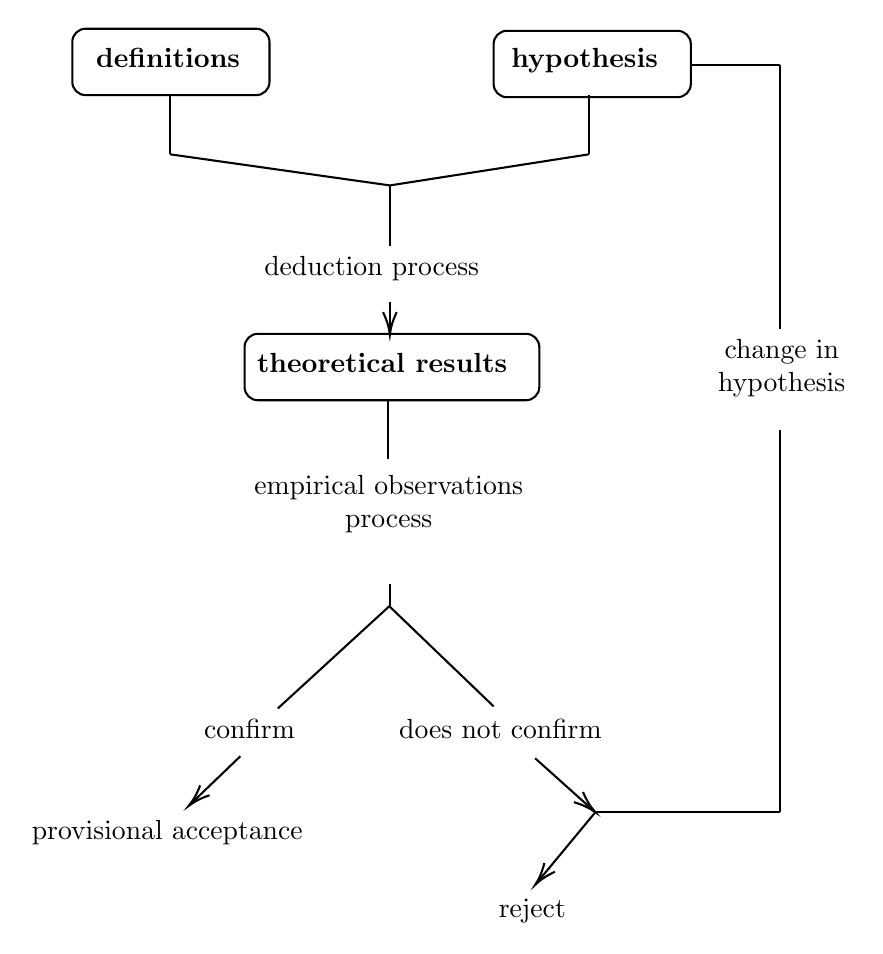
\begin{tikzpicture}[x=0.75pt,y=0.75pt,yscale=-1,xscale=1]
		%uncomment if require: \path (0,673); %set diagram left start at 0, and has height of 673
		
		%Rounded Rect [id:dp450071796993355] 
		\draw   (79,93.4) .. controls (79,89.87) and (81.87,87) .. (85.4,87) -- (167.6,87) .. controls (171.13,87) and (174,89.87) .. (174,93.4) -- (174,112.6) .. controls (174,116.13) and (171.13,119) .. (167.6,119) -- (85.4,119) .. controls (81.87,119) and (79,116.13) .. (79,112.6) -- cycle ;
		%Rounded Rect [id:dp3123365770289972] 
		\draw   (282,94.4) .. controls (282,90.87) and (284.87,88) .. (288.4,88) -- (370.6,88) .. controls (374.13,88) and (377,90.87) .. (377,94.4) -- (377,113.6) .. controls (377,117.13) and (374.13,120) .. (370.6,120) -- (288.4,120) .. controls (284.87,120) and (282,117.13) .. (282,113.6) -- cycle ;
		%Straight Lines [id:da7011194954020175] 
		\draw    (126,119) -- (126,147.5) ;
		%Straight Lines [id:da8062705329606052] 
		\draw    (328,119) -- (328,147.5) ;
		%Straight Lines [id:da854985017000603] 
		\draw    (126,147.5) -- (232,162.5) ;
		%Straight Lines [id:da5150789261033402] 
		\draw    (232,162.5) -- (328,147.5) ;
		%Straight Lines [id:da2480035607158091] 
		\draw    (232,163) -- (232,191.5) ;
		%Rounded Rect [id:dp37324890998767835] 
		\draw   (162,240.4) .. controls (162,236.87) and (164.87,234) .. (168.4,234) -- (297.6,234) .. controls (301.13,234) and (304,236.87) .. (304,240.4) -- (304,259.6) .. controls (304,263.13) and (301.13,266) .. (297.6,266) -- (168.4,266) .. controls (164.87,266) and (162,263.13) .. (162,259.6) -- cycle ;
		%Straight Lines [id:da44914926894106055] 
		\draw    (231,266) -- (231,294.5) ;
		%Straight Lines [id:da48173791567363056] 
		\draw    (232,218.5) -- (232,232.5) ;
		\draw [shift={(232,234.5)}, rotate = 270] [color={rgb, 255:red, 0; green, 0; blue, 0 }  ][line width=0.75]    (10.93,-3.29) .. controls (6.95,-1.4) and (3.31,-0.3) .. (0,0) .. controls (3.31,0.3) and (6.95,1.4) .. (10.93,3.29)   ;
		%Straight Lines [id:da174728449205225] 
		\draw    (232,365) -- (192.54,401.18) -- (178,414.5) ;
		%Straight Lines [id:da20423642856626523] 
		\draw    (282,413.5) -- (232,365.5) ;
		%Straight Lines [id:da5612344595082037] 
		\draw    (160,437.5) -- (136.44,460.11) ;
		\draw [shift={(135,461.5)}, rotate = 316.17] [color={rgb, 255:red, 0; green, 0; blue, 0 }  ][line width=0.75]    (10.93,-3.29) .. controls (6.95,-1.4) and (3.31,-0.3) .. (0,0) .. controls (3.31,0.3) and (6.95,1.4) .. (10.93,3.29)   ;
		%Straight Lines [id:da8929748054583597] 
		\draw    (302,438.5) -- (329.51,463.16) ;
		\draw [shift={(331,464.5)}, rotate = 221.88] [color={rgb, 255:red, 0; green, 0; blue, 0 }  ][line width=0.75]    (10.93,-3.29) .. controls (6.95,-1.4) and (3.31,-0.3) .. (0,0) .. controls (3.31,0.3) and (6.95,1.4) .. (10.93,3.29)   ;
		%Straight Lines [id:da720094639073076] 
		\draw    (331,464.5) -- (303.28,497.96) ;
		\draw [shift={(302,499.5)}, rotate = 309.64] [color={rgb, 255:red, 0; green, 0; blue, 0 }  ][line width=0.75]    (10.93,-3.29) .. controls (6.95,-1.4) and (3.31,-0.3) .. (0,0) .. controls (3.31,0.3) and (6.95,1.4) .. (10.93,3.29)   ;
		%Straight Lines [id:da3810332730221839] 
		\draw    (420,464.5) -- (420,280.5) ;
		%Straight Lines [id:da48862321771791284] 
		\draw    (331,464.5) -- (420,464.5) ;
		%Straight Lines [id:da920299974696865] 
		\draw    (377,104.5) -- (420,104.5) ;
		%Straight Lines [id:da014842651548173658] 
		\draw    (420,231.5) -- (420,136.5) -- (420,104.5) ;
		%Straight Lines [id:da589053840154339] 
		\draw    (232,354.75) -- (232,365.5) ;
		
		% Text Node
		\draw (89,95) node [anchor=north west][inner sep=0.75pt]   [align=left] {\textbf{definitions}};
		% Text Node
		\draw (289,95) node [anchor=north west][inner sep=0.75pt]   [align=left] {\textbf{hypothesis}};
		% Text Node
		\draw (170,195) node [anchor=north west][inner sep=0.75pt]   [align=left] {deduction process};
		% Text Node
		\draw (166.5,242) node [anchor=north west][inner sep=0.75pt]   [align=left] {\textbf{theoretical results}};
		% Text Node
		\draw (160.5,300.5) node [anchor=north west][inner sep=0.75pt]   [align=left] {\begin{minipage}[lt]{104.2pt}\setlength\topsep{0pt}
		\begin{center}
		empirical observations\\process
		\end{center}
		
		\end{minipage}};
		% Text Node
		\draw (141,418) node [anchor=north west][inner sep=0.75pt]   [align=left] {confirm};
		% Text Node
		\draw (235,418) node [anchor=north west][inner sep=0.75pt]   [align=left] {does not confirm};
		% Text Node
		\draw (58,467) node [anchor=north west][inner sep=0.75pt]   [align=left] {provisional acceptance};
		% Text Node
		\draw (283,505) node [anchor=north west][inner sep=0.75pt]   [align=left] {reject};
		% Text Node
		\draw (385,235) node [anchor=north west][inner sep=0.75pt]   [align=left] {\begin{minipage}[lt]{51.49pt}\setlength\topsep{0pt}
		\begin{center}
		change in \\hypothesis
		\end{center}
		
		\end{minipage}};
		\end{tikzpicture}
	\end{figure}
	
	It must also be known to the reader that we insist on the fact that real scientists should no have emotions behind the subjects they study or speak about. They have to only use evidence (facts based on data, peer-review, reproducible experiences, consensus of scientific community) rather than emotional, biased\footnote{Among all major biases that we will introduce later, the Confirmation Bias - the tendency to search for, interpret, favour, and recall information that confirms or supports one's prior personal beliefs or values - is very likely the most common by scientifically illiterate people.}, subjective educational individual analysis that are not data driven. Obviously we may question the assumption that the used sensory probes detect something real or not? But professional scientists don't care about such a philosophical question. The only thing that matters (putting a part the fun of it...) is that these sensory probes give reliable, useful and consistent measures to test models that will help to build new tools for humanity!

	\begin{figure}[H]
		\centering
		\includegraphics[scale=0.5]{img/intro/consenus_religions.jpg}
		\caption[]{An example of absence of consensus in a small sample of religions}
	\end{figure}
	Notice also a funny shape of scientific $10$ commandments:
	\begin{enumerate}
		\item The phenomena you will observe\\
		And never measures you will falsify\\
		(attention to the confirmation bias\footnote{It's very strongly advised to read our introduction to cognitive biases in the section of Decision Theory page \pageref{cognitive bias}}!)
		
		\item Hypothesis you will proposed\\
		That with experiment you will test
		
		\item The experiment precisely you will describe and the data and algorithms you will provide\\
		Because your colleague will reproduce it\\
		(attention to the narrative discipline trap: the facts will be fitted to the desired results)
		
		\item With your results\\
		A theory you will build
		
		\item Parsimony you will use\\
		And the simplest hypothesis you will retain
		
		\item Ultimate truth will never be (epistemic humility)\\
		And always you will search for the truth
		
		\item From a non-refutable thesis you will refrain\\
		Because outside of the science it will remain
		
		\item All failures will be like a success\\
		Because science can confirm but also invalidate
		
		\item My authority I will not use (authority bias)\\
		To bias people opinions in fields where I have no proven expertise
		
		\item The Archimedean Oath and the Scientific Publication Rules I will respect\\
		As science must be transparent and responsible
	\end{enumerate}
	
	\begin{fquote}[Dara Ó Brian]Science knows it doesn't know everything, otherwise it would stop.
 	\end{fquote}

	\begin{tcolorbox}[enhanced,colback=red!5!white,colframe=black!50!red,boxrule=1pt,arc=0pt,outer arc=0pt,drop lifted shadow,after skip=10pt plus 2pt]
	\bcbombe Caution! It is very easy to make new physical theories by just aligning words. This is named "\NewTerm{philosophy}\index{philosophy}" or "\NewTerm{rhetoric}\index{rhetoric}" and the Greeks thought of the atoms in this method. This can lead with a lot of luck to a true theory. Against it is much more difficult to make a "\NewTerm{predictive theory}"\index{predictive theory}, that is to say with equations that predict the outcome of an experiment (all physical theories must posit a correspondence between their mathematical apparatus and the physical world that they are attempting to describe).\\
	
	Moreover many philosophers reinvent arguments physicists have long known to be wrong. We have heard philosophers worry about paradoxes physicists solved ages ago, and we have heard philosophers deduce how natural laws should be while ignoring how natural laws are. In short, there are unfortunately many philosophers who don't notice when they are out of their depth. The same can be said of physicists, though. Some physicists draw on philosophical arguments more frequently than they like to admit. It's easy enough however for us to discard philosophy as useful - because it is useless.
	\end{tcolorbox}
	
	\begin{fquote}[L. Aron Nelson]Science doesn't know everything, religion doesn't know anything!
 	\end{fquote}

	\begin{tcolorbox}[title=Remark,arc=10pt,breakable,drop lifted shadow,
  skin=enhanced,
  skin first is subskin of={enhancedfirst}{arc=10pt,no shadow},
  skin middle is subskin of={enhancedmiddle}{arc=10pt,no shadow},
  skin last is subskin of={enhancedlast}{drop lifted shadow}]
	What separates mathematics and physics is that in mathematics, the hypothesis is always true. Mathematical discourse is not a proof of an external seeking truth, but a target of consistency. What should be correct is just the reasoning. 
	\end{tcolorbox}
	
	\begin{fquote}[Matt Blaze]When people say "The reason you can't trust science is that scientists used to say <thing that turned out be wrong> but now they say <different thing>", they are actually explaining why science works so well!
 	\end{fquote}

	When these rules are not respected, we speak of "\NewTerm{scientific fraud}"\index{scientific fraud} or of "\NewTerm{intellectual fraud}" (which often leads to being fired from his job but unfortunately we still not retired the diplomas when it happens). In general, scientific fraud itself comes in four main forms: plagiarism, fabrication of data and alteration of results unfavourable to the hypothesis, the omission of clear working hypotheses and collected datas, fallacious and biased arguments (remember that especially a rhetorical argument that isn't backed up by experimental evidence has no interest for professional scientists!). To these frauds we can also add behaviours that pose problems regarding to the quality of work or more specifically to ethics, such as  submitting for example several times the same publication with only a few modifications, the omission of conflict of interest (financial, religious, political), the dangerous experiments, the non-conservation of primary data, etc.
	\begin{figure}[H]
		\centering
		\includegraphics[scale=0.5]{img/intro/peer_review.jpg}
		\caption[]{Source: \url{http://cartoonsbyjosh.co.uk}}
	\end{figure}	

	\subsection{Descartes' Method}
	Now we present the four principles of the Descartes' method which, as remind, is considered as the first scientist in history by his method of analysis:
	\begin{itemize}
		\item[P1.] Never accept anything as true that I obviously knew to be such. That is to say, carefully avoid precipitation and to understand nothing more in my judgements than what would appear so clearly and distinctly to my mind, that I had no occasion to doubt.
		
		\item[P2.] Divide each of the difficulties I have to examine into as many parts as possible (scrupulous observations and plausible hypothesis until evidence of the opposite), and that would be required to resolve them in the best way.
		
		\item[P3.] Driving my thoughts in order, beginning with the simplest objects and easiest to know, to go up gradually by degrees to the knowledge of the most compounds, and even assuming the order between those who not naturally precede each other.
		
		\item[P4.] Make everywhere so complete enumerations and so general reviews, that I'm sure not to omit anything.
	\end{itemize}
	\begin{figure}[H]
		\centering
		\includegraphics[scale=0.3]{img/intro/nullius_in_verba.jpg}
	\end{figure}
	\textit{Nullius in verba} (Latin for "on the word of no one" or "take nobody's word for it") is the motto of the Royal Society.  It is an expression of the determination of Fellows to withstand the domination of authority and to verify all statements by an appeal to facts determined by reproducible experiments and by cautious scientific peer-review\footnote{The process of peer-review generally applies to journal articles, but it is possible for a book to be peer-reviewed as well. Although many books go through some sort of editorial or review process, there is not an easy method for determining whether a book is peer reviewed. One method for locating peer-reviewed books is to take a look at book publications from university presses. Books published by university presses almost always go through a process of peer-review. Books from university presses are typically written by faculty members are who are under immense pressure to produce authoritative scholarly literature. The process of peer-review for university presses typically involves two or three independent referees who will initially review the manuscript. If the manuscript receives positive review, the university press will send it to their editorial board, who are all faculty members, for final review.}.

	\subsubsection{Blind studies}
	Scientific experiments\footnote{This text is a copy/paste of an article written by Manuel Gnida at \url{http://www.symmetrymagazine.org/article/the-facts-and-nothing-but-the-facts}} are designed to determine facts about our world using either "\NewTerm{retrospective studies}\index{retrospective studies}" based on the search of correlations by exploiting existing databases (hence looks backwards) or "\NewTerm{prospective studies}\footnote{Prospective studies have usually fewer potential sources of bias and confounding than retrospective studies.}\index{prospective studies}" based on the search of causalities using controlled/randomized/double-blinded experiments (respectively frequently abbreviated RCT or RCDBT where the "T" stand for "Trial" instead of using the word "Experiment" or "Study"\index{randomized controlled trial}). But in complicated analyses, there's a risk that researchers will unintentionally skew results to match what they were expecting to find. To reduce or eliminate this potential bias, scientists apply a method known as "\NewTerm{blind analysis}\index{blind analysis}".
	
	Blind studies are probably best known from their use in clinical drug trials\footnote{The simplest trial design is a "single-arm trial". In this design, a sample of individuals with the targeted medical condition is given the experimental therapy and then followed over time to observe their response. In a "double-arm trial" half of the people will receive a placebo (exposure group vs non-exposure group). In a "triple-arm trial" a third will receive a competitive treatment. In the general case we speak of "multi-arm trial".} (the term "triple-blinding" sometimes refers to this), in which patients are kept in the dark about - or blind to - whether they're receiving an actual drug or a placebo\footnote{In the science of drugs, a "pure placebo" is a treatment without any active substance; an "impure placebo" is a pharmacologically active product but having no effect on the pathology treated, or whose efficacy has \underline{not been sufficiently demonstrated}.} (indeed dummy pills, with no pharmacological activity at all, demonstrably improve health at a low statistical level of significance that is why double-blind drug trials must use placebos as controls to neutralize the placebo effect and permit the blinding of the treatment) but also the doctors themselves (to minimize behavioural bias) and the people who collects the data (to minimize the corruption), we speak then of "\NewTerm{double-bline randomised placebo controlled trial}\index{double-bline randomised placebo controlled trial}". This approach helps researchers judge whether their results stem from the treatment itself or from the patients' belief that they are receiving it. But the method is also use in Gastronomy tasting or in forensic laboratories as well.
	
	Particle physicists and astrophysicists do blind studies, too!!! The approach is particularly valuable when scientists search for extremely small effects hidden among background noise that point to the existence of something new, not accounted for in the current model. Examples include the much-publicized discoveries of the Higgs boson by experiments at CERN's Large Hadron Collider\footnote{If you doubt of the utility in every day life of the CERN, just keep in mind that it is in this fundamental research center that the world wide web has been invented, but also touch-screens, tracker balls, robust chips for nuclear power plants, bid data visualisation softwares, hybrid pixelated detectors, gas electron multiplier, superconductivity technologies for tokamaks and nuclear magnetic resonance scanner, etc.} and of gravitational waves by the Advanced LIGO detector.
	
	«\textit{Scientific analyses are iterative processes, in which we make a series of small adjustments to theoretical models until the models accurately describe the experimental data}» says Elisabeth Krause, a postdoc at the Kavli Institute for Particle Astrophysics and Cosmology, which is jointly operated by Stanford University and the Department of Energy's SLAC National Accelerator Laboratory. «\textit{At each step of an analysis, there is the danger that prior knowledge guides the way we make adjustments. Blind analyses help us make independent and better decisions}».
	
	Return on experience (REX) shows as expected that blind analyses need to be designed individually for each experiment. The way the blinding is done needs to leave researchers with enough information to allow a meaningful analysis, and it depends on the type of data coming out of a specific experiment.

	A common approach is to base the analysis on only some of the data, excluding the part in which an anomaly is thought to be hiding. The excluded data is said to be in a "black box" or "hidden signal box".

	Take the search for the Higgs boson. Using data collected with the Large Hadron Collider until the end of 12011 (holocene calendar), researchers saw hints of a bump as a potential sign of a new particle with a mass of about $125$ gigaelectronvolts. So when they looked at new data, they deliberately quarantined the mass range around this bump and focused on the remaining data instead.
	\label{evidence levels chart}\index{evidence levels}
	\begin{figure}[H]
		\centering
		\resizebox{\textwidth}{!}{%
		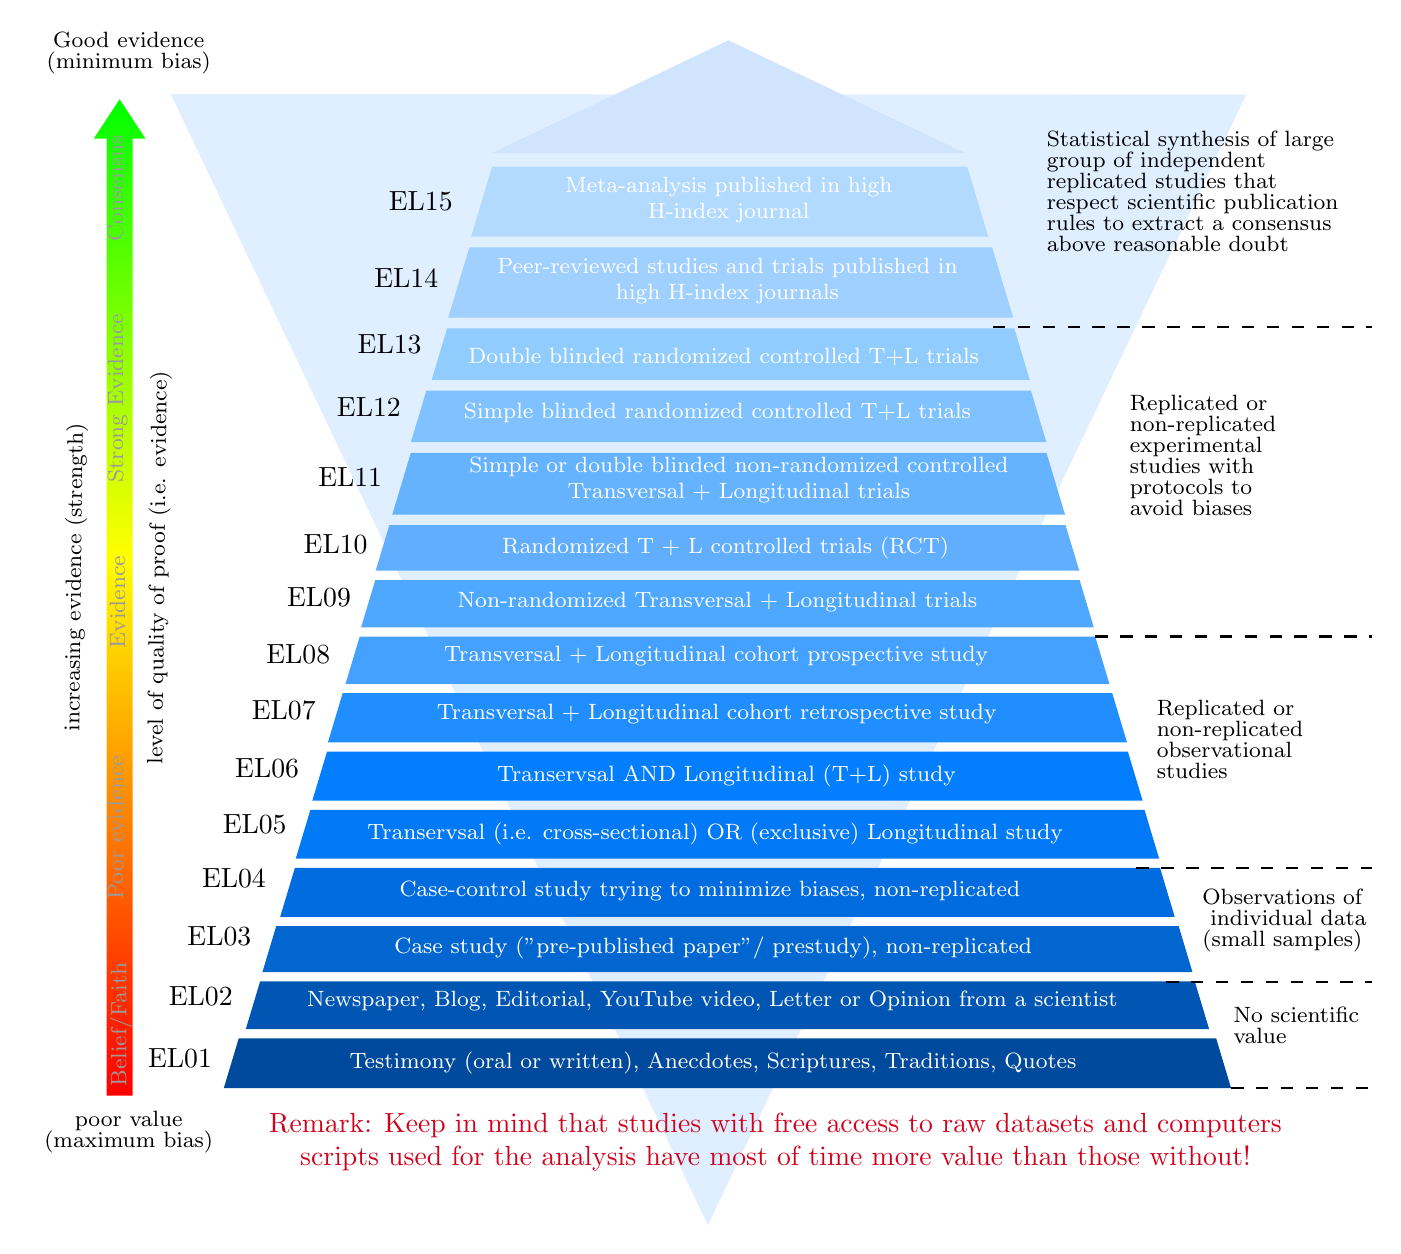
\begin{tikzpicture}[x=0.75pt,y=0.75pt,yscale=-1,xscale=1,scale=1]
		%uncomment if require: \path (0,728); %set diagram left start at 0, and has height of 728
		
		% Gradient Info
  
		\tikzset {_i3725vhd5/.code = {\pgfsetadditionalshadetransform{ \pgftransformshift{\pgfpoint{0 bp } { 0 bp }  }  \pgftransformrotate{-90 }  \pgftransformscale{2 }  }}}
		\pgfdeclarehorizontalshading{_a1bw0ltp0}{150bp}{rgb(0bp)=(0,1,0);
		rgb(37.5bp)=(0,1,0);
		rgb(48.92857142857143bp)=(1,1,0);
		rgb(62.410714285714285bp)=(1,0,0);
		rgb(100bp)=(1,0,0)}
		\tikzset{every picture/.style={line width=0.75pt}} %set default line width to 0.75pt        
		
		%Up Arrow [id:dp05602383554319279] 
		\draw  [draw opacity=0][shading=_a1bw0ltp0,_i3725vhd5] (32.3,60) -- (44.8,41) -- (57.3,60) -- (51.05,60) -- (51.05,521) -- (38.55,521) -- (38.55,60) -- cycle ;
		%Shape: Triangle [id:dp9708421993657637] 
		\draw  [draw opacity=0][fill={rgb, 255:red, 224; green, 239; blue, 255 }  ,fill opacity=1 ] (328.22,583.46) -- (69.43,38.47) -- (587.59,38.74) -- cycle ;
		%Shape: Trapezoid [id:dp5460408456551786] 
		\draw  [draw opacity=0][fill={rgb, 255:red, 0; green, 74; blue, 157 }  ,fill opacity=1 ] (95,517.4) -- (102.2,493.4) -- (573.1,493.4) -- (580.3,517.4) -- cycle ;
		%Straight Lines [id:da666965770030949] 
		\draw  [dash pattern={on 4.5pt off 4.5pt}]  (580.3,517.4) -- (648.3,517.4) ;
		%Shape: Trapezoid [id:dp7878447116277159] 
		\draw  [draw opacity=0][fill={rgb, 255:red, 0; green, 86; blue, 178 }  ,fill opacity=1 ] (105.6,488.95) -- (112.49,466) -- (562.81,466) -- (569.7,488.95) -- cycle ;
		%Shape: Trapezoid [id:dp7124042957050283] 
		\draw  [draw opacity=0][fill={rgb, 255:red, 2; green, 102; blue, 208 }  ,fill opacity=1 ] (113.6,461.54) -- (120.25,439.38) -- (555.05,439.38) -- (561.7,461.54) -- cycle ;
		%Shape: Trapezoid [id:dp38197977873265176] 
		\draw  [draw opacity=0][fill={rgb, 255:red, 1; green, 107; blue, 224 }  ,fill opacity=1 ] (122.15,434.92) -- (129.22,411.35) -- (546.08,411.35) -- (553.15,434.92) -- cycle ;
		%Shape: Trapezoid [id:dp7280774584097203] 
		\draw  [draw opacity=0][fill={rgb, 255:red, 2; green, 121; blue, 246 }  ,fill opacity=1 ] (129.65,406.89) -- (136.72,383.32) -- (538.58,383.32) -- (545.65,406.89) -- cycle ;
		%Shape: Trapezoid [id:dp5825969174008463] 
		\draw  [draw opacity=0][fill={rgb, 255:red, 2; green, 126; blue, 255 }  ,fill opacity=1 ] (137.65,378.86) -- (144.72,355.3) -- (530.58,355.3) -- (537.65,378.86) -- cycle ;
		%Shape: Trapezoid [id:dp5470980977975435] 
		\draw  [draw opacity=0][fill={rgb, 255:red, 33; green, 142; blue, 255 }  ,fill opacity=1 ] (145.15,350.84) -- (152.28,327.07) -- (523.02,327.07) -- (530.15,350.84) -- cycle ;
		%Straight Lines [id:da34095757385692127] 
		\draw  [dash pattern={on 4.5pt off 4.5pt}]  (549,466.4) -- (648.3,466.4) ;
		%Straight Lines [id:da6109070957996154] 
		\draw  [dash pattern={on 4.5pt off 4.5pt}]  (534.7,411.4) -- (648.3,411.4) ;
		%Shape: Trapezoid [id:dp9834861839130156] 
		\draw  [draw opacity=0][fill={rgb, 255:red, 68; green, 161; blue, 255 }  ,fill opacity=1 ] (153.65,322.61) -- (160.48,299.84) -- (514.82,299.84) -- (521.65,322.61) -- cycle ;
		%Shape: Trapezoid [id:dp3355704515070128] 
		\draw  [draw opacity=0][fill={rgb, 255:red, 78; green, 168; blue, 255 }  ,fill opacity=1 ] (161.15,295.38) -- (167.98,272.61) -- (507.32,272.61) -- (514.15,295.38) -- cycle ;
		%Shape: Trapezoid [id:dp11167634755282863] 
		\draw  [draw opacity=0][fill={rgb, 255:red, 97; green, 173; blue, 254 }  ,fill opacity=1 ] (168.15,268.15) -- (174.74,246.2) -- (500.56,246.2) -- (507.15,268.15) -- cycle ;
		%Shape: Trapezoid [id:dp08176288644867191] 
		\draw  [draw opacity=0][fill={rgb, 255:red, 101; green, 178; blue, 255 }  ,fill opacity=1 ] (176.15,241.15) -- (185.08,211.4) -- (491.37,211.4) -- (500.3,241.15) -- cycle ;
		%Shape: Trapezoid [id:dp8024788039902053] 
		\draw  [draw opacity=0][fill={rgb, 255:red, 128; green, 193; blue, 255 }  ,fill opacity=1 ] (185.15,206.15) -- (192.58,181.4) -- (483.87,181.4) -- (491.3,206.15) -- cycle ;
		%Shape: Trapezoid [id:dp21283867910389387] 
		\draw  [draw opacity=0][fill={rgb, 255:red, 145; green, 204; blue, 255 }  ,fill opacity=1 ] (195.15,176.15) -- (202.58,151.4) -- (475.87,151.4) -- (483.3,176.15) -- cycle ;
		%Shape: Trapezoid [id:dp7877216348244722] 
		\draw  [draw opacity=0][fill={rgb, 255:red, 160; green, 208; blue, 255 }  ,fill opacity=1 ] (203.15,146.15) -- (213.28,112.4) -- (465.17,112.4) -- (475.3,146.15) -- cycle ;
		%Shape: Trapezoid [id:dp979911441394272] 
		\draw  [draw opacity=0][fill={rgb, 255:red, 178; green, 218; blue, 255 }  ,fill opacity=1 ] (214.15,107.15) -- (224.28,73.4) -- (453.17,73.4) -- (463.3,107.15) -- cycle ;
		%Shape: Triangle [id:dp35920379810540126] 
		\draw  [draw opacity=0][fill={rgb, 255:red, 208; green, 228; blue, 253 }  ,fill opacity=1 ] (338.15,12.6) -- (452.3,67) -- (224,67) -- cycle ;
		%Straight Lines [id:da012029472901313731] 
		\draw  [dash pattern={on 4.5pt off 4.5pt}]  (514.82,299.84) -- (648.3,299.84) ;
		%Straight Lines [id:da832925117575892] 
		\draw  [dash pattern={on 4.5pt off 4.5pt}]  (465.52,150.84) -- (648.3,150.84) ;
		
		% Text Node
		\draw (96,528) node [anchor=north west][inner sep=0.75pt]   [align=left] {\begin{minipage}[lt]{395pt}\setlength\topsep{0pt}
		\begin{center}
		\textcolor[rgb]{0.82,0.01,0.11}{Remark: Keep in mind that studies with free access to raw datasets and computers}\\\textcolor[rgb]{0.82,0.01,0.11}{scripts used for the analysis have most of time more value than those without!}
		\end{center}
		
		\end{minipage}};
		% Text Node
		\draw (1,527) node [anchor=north west][inner sep=0.75pt]   [align=left] [font=\footnotesize\linespread{0.8}\selectfont] {\begin{minipage}[lt]{70pt}\setlength\topsep{0pt}
		\begin{center}
		{poor value}\\{(maximum bias)}
		\end{center}
		
		\end{minipage}};
		% Text Node
		\draw (1,7) node [anchor=north west][inner sep=0.75pt]   [align=left] [font=\footnotesize\linespread{0.8}\selectfont] {\begin{minipage}[lt]{70pt}\setlength\topsep{0pt}
		\begin{center}
		{Good evidence}\\{(minimum bias)}
		\end{center}
		
		\end{minipage}};
		% Text Node
		\draw (15.85,346.9) node [anchor=north west][inner sep=0.75pt]  [font=\footnotesize,rotate=-270.65] [align=left] {increasing evidence (strength)};
		% Text Node
		\draw (55.85,362.9) node [anchor=north west][inner sep=0.75pt]  [font=\footnotesize,rotate=-270.65] [align=left] {level of quality of proof (i.e. evidence)};
		% Text Node
		\draw (38.55,518) node [anchor=north west][inner sep=0.75pt]  [font=\footnotesize,color={rgb, 255:red, 155; green, 155; blue, 155 }  ,opacity=1 ,rotate=-270] [align=left] {Belief/Faith};
		% Text Node
		\draw (37.55,428) node [anchor=north west][inner sep=0.75pt]  [font=\footnotesize,color={rgb, 255:red, 155; green, 155; blue, 155 }  ,opacity=1 ,rotate=-270] [align=left] {Poor evidence};
		% Text Node
		\draw (38.55,307) node [anchor=north west][inner sep=0.75pt]  [font=\footnotesize,color={rgb, 255:red, 155; green, 155; blue, 155 }  ,opacity=1 ,rotate=-270] [align=left] {Evidence};
		% Text Node
		\draw (37.55,227) node [anchor=north west][inner sep=0.75pt]  [font=\footnotesize,color={rgb, 255:red, 155; green, 155; blue, 155 }  ,opacity=1 ,rotate=-270] [align=left] {Strong Evidence};
		% Text Node
		\draw (37.55,111) node [anchor=north west][inner sep=0.75pt]  [font=\footnotesize,color={rgb, 255:red, 155; green, 155; blue, 155 }  ,opacity=1 ,rotate=-270] [align=left] {Consensus};
		% Text Node
		\draw (154.15,498.4) node [anchor=north west][inner sep=0.75pt]  [font=\footnotesize,color={rgb, 255:red, 255; green, 255; blue, 255 }  ,opacity=1 ] [align=left] {Testimony (oral or written), Anecdotes, Scriptures, Traditions, Quotes};
		% Text Node
		\draw (57,497) node [anchor=north west][inner sep=0.75pt]   [align=left] {EL01};
		% Text Node
		\draw (133.65,469.4) node [anchor=north west][inner sep=0.75pt]  [font=\footnotesize,color={rgb, 255:red, 255; green, 255; blue, 255 }  ,opacity=1 ] [align=left] {Newspaper, Blog, Editorial, YouTube video, Letter or Opinion from a scientist};
		% Text Node
		\draw (67,467) node [anchor=north west][inner sep=0.75pt]   [align=left] {EL02};
		% Text Node
		\draw (175.65,443) node [anchor=north west][inner sep=0.75pt]  [font=\footnotesize,color={rgb, 255:red, 255; green, 255; blue, 255 }  ,opacity=1 ] [align=left] {Case study ("pre-published paper"/ prestudy), non-replicated};
		% Text Node
		\draw (76,438) node [anchor=north west][inner sep=0.75pt]   [align=left] {EL03};
		% Text Node
		\draw (83,410) node [anchor=north west][inner sep=0.75pt]   [align=left] {EL04};
		% Text Node
		\draw (178.15,416) node [anchor=north west][inner sep=0.75pt]  [font=\footnotesize,color={rgb, 255:red, 255; green, 255; blue, 255 }  ,opacity=1 ] [align=left] {Case-control study trying to minimize biases, non-replicated};
		% Text Node
		\draw (162.65,388) node [anchor=north west][inner sep=0.75pt]  [font=\footnotesize,color={rgb, 255:red, 255; green, 255; blue, 255 }  ,opacity=1 ] [align=left] {Transervsal (i.e. cross-sectional) OR (exclusive) Longitudinal study};
		% Text Node
		\draw (93,384) node [anchor=north west][inner sep=0.75pt]   [align=left] {EL05};
		% Text Node
		\draw (99,357) node [anchor=north west][inner sep=0.75pt]   [align=left] {EL06};
		% Text Node
		\draw (225.15,360) node [anchor=north west][inner sep=0.75pt]  [font=\footnotesize,color={rgb, 255:red, 255; green, 255; blue, 255 }  ,opacity=1 ] [align=left] {Transervsal AND Longitudinal (T+L) study};
		% Text Node
		\draw (107,329) node [anchor=north west][inner sep=0.75pt]   [align=left] {EL07};
		% Text Node
		\draw (580,477) node [anchor=north west][inner sep=0.75pt]   [align=left] [font=\footnotesize\linespread{0.8}\selectfont] {{No scientific}\\{value}};
		% Text Node
		\draw (565,420) node [anchor=north west][inner sep=0.75pt]   [align=left] [font=\footnotesize\linespread{0.8}\selectfont] {{Observations of}\\{ individual data }\\{(small samples)}};
		% Text Node
		\draw (196.15,331) node [anchor=north west][inner sep=0.75pt]  [font=\footnotesize,color={rgb, 255:red, 255; green, 255; blue, 255 }  ,opacity=1 ] [align=left] {Transversal + Longitudinal cohort retrospective study};
		% Text Node
		\draw (114,302) node [anchor=north west][inner sep=0.75pt]   [align=left] {EL08};
		% Text Node
		\draw (199.65,303) node [anchor=north west][inner sep=0.75pt]  [font=\footnotesize,color={rgb, 255:red, 255; green, 255; blue, 255 }  ,opacity=1 ] [align=left] {Transversal + Longitudinal cohort prospective study};
		% Text Node
		\draw (124,275) node [anchor=north west][inner sep=0.75pt]   [align=left] {EL09};
		% Text Node
		\draw (206.15,277) node [anchor=north west][inner sep=0.75pt]  [font=\footnotesize,color={rgb, 255:red, 255; green, 255; blue, 255 }  ,opacity=1 ] [align=left] {Non-randomized Transversal + Longitudinal trials};
		% Text Node
		\draw (132,249) node [anchor=north west][inner sep=0.75pt]   [align=left] {EL10};
		% Text Node
		\draw (227.65,250.2) node [anchor=north west][inner sep=0.75pt]  [font=\footnotesize,color={rgb, 255:red, 255; green, 255; blue, 255 }  ,opacity=1 ] [align=left] {Randomized T + L controlled trials (RCT)};
		% Text Node
		\draw (139,217) node [anchor=north west][inner sep=0.75pt]   [align=left] {EL11};
		% Text Node
		\draw (195,212) node [anchor=north west][inner sep=0.75pt]  [font=\footnotesize,color={rgb, 255:red, 255; green, 255; blue, 255 }  ,opacity=1 ] [align=left] {\begin{minipage}[lt]{220pt}\setlength\topsep{0pt}
		\begin{center}
		Simple or double blinded non-randomized controlled\\Transversal + Longitudinal trials
		\end{center}
		
		\end{minipage}};
		% Text Node
		\draw (148,183) node [anchor=north west][inner sep=0.75pt]   [align=left] {EL12};
		% Text Node
		\draw (198,186) node [anchor=north west][inner sep=0.75pt]  [font=\footnotesize,color={rgb, 255:red, 255; green, 255; blue, 255 }  ,opacity=1 ] [align=left] {\begin{minipage}[lt]{200pt}\setlength\topsep{0pt}
		\begin{center}
		Simple blinded randomized controlled T+L trials
		\end{center}
		
		\end{minipage}};
		% Text Node
		\draw (158,153) node [anchor=north west][inner sep=0.75pt]   [align=left] {EL13};
		% Text Node
		\draw (201,159.4) node [anchor=north west][inner sep=0.75pt]  [font=\footnotesize,color={rgb, 255:red, 255; green, 255; blue, 255 }  ,opacity=1 ] [align=left] {\begin{minipage}[lt]{200pt}\setlength\topsep{0pt}
		\begin{center}
		Double blinded randomized controlled T+L trials
		\end{center}
		
		\end{minipage}};
		% Text Node
		\draw (216.15,116) node [anchor=north west][inner sep=0.75pt]  [font=\footnotesize,color={rgb, 255:red, 255; green, 255; blue, 255 }  ,opacity=1 ] [align=left] {\begin{minipage}[lt]{180pt}\setlength\topsep{0pt}
		\begin{center}
		Peer-reviewed studies and trials published in \\high H-index journals
		\end{center}
		
		\end{minipage}};
		% Text Node
		\draw (166,121) node [anchor=north west][inner sep=0.75pt]   [align=left] {EL14};
		% Text Node
		\draw (173,84) node [anchor=north west][inner sep=0.75pt]   [align=left] {EL15};
		% Text Node
		\draw (250.15,77) node [anchor=north west][inner sep=0.75pt]  [font=\footnotesize,color={rgb, 255:red, 255; green, 255; blue, 255 }  ,opacity=1 ] [align=left] {\begin{minipage}[lt]{130pt}\setlength\topsep{0pt}
		\begin{center}
		Meta-analysis published in high\\H-index journal
		\end{center}
		
		\end{minipage}};
		% Text Node
		\draw (543,329) node [anchor=north west][inner sep=0.75pt]  [font=\footnotesize\linespread{0.8}\selectfont] [align=left] {Replicated or \\non-replicated \\observational \\studies};
		% Text Node
		\draw (530,182) node [anchor=north west][inner sep=0.75pt]  [font=\footnotesize\linespread{0.8}\selectfont] [align=left] {Replicated or \\non-replicated \\experimental \\studies with \\protocols to\\avoid biases};
		% Text Node
\draw (490,55) node [anchor=north west][inner sep=0.75pt]  [font=\footnotesize\linespread{0.8}\selectfont] [align=left] {Statistical synthesis of large\\group of independent \\replicated studies that \\respect scientific publication\\rules to extract a consensus \\above reasonable doubt};
		
		\end{tikzpicture}
		}%
		
		\vspace*{1mm}
		\caption{Scientific evidence hierarchy (assuming each level is made “at its best”)}
	\end{figure}
	
	The figure above\footnote{The huge majority of techniques and methods mentioned in each of the rows of the figure are proven and explained in the section Statistics starting from page \pageref{statistics} and in the section of Numerical methods starting from page \pageref{regression techniques}.} that applies to multiple fields of Science (physics, chemistry, biology, genetics, epidemiology, social science, economy, psychology, archaeology, astrophysics, astronomy, cosmology, epidemiology) illustrates in the lowest level of evidence EL01 the obvious fact that we should never trust the opinions and beliefs of scientists (even less "corporate scientists"...), physicians, doctors and engineers (these latter are not scientists by the way, see for example \cite{smith2004doctors} and \cite{freed2004doctors}!) - because science must not be driven by humans beliefs and opinions (!) - but only by the evidence provided by the \textbf{\underline{DATA}} from reproducible independent experiments provided with their statistical analysis at a meta-analysis level in high H-index (HI) and high Impact Factor (IF) peer-reviewed papers!
	
	\begin{tcolorbox}[enhanced,colback=red!5!white,colframe=black!50!red,boxrule=1pt,arc=0pt,outer arc=0pt,drop lifted shadow,after skip=10pt plus 2pt]
	\bcbombe Caution! We can find on Internet plenty of professional looking websites administered by anonymous people (that try hard to hide who they are, in what country they live and what business they run...) compiling meta-analysis! However a website that is anonymous - having by definition a zero H-index - is obviously suspect especially when they cherry-pick only studies that goes in the direction of their political and religious agenda and don't provide the source code to reproduce the results. The same goes for some books that want to pass themselves off as textbooks and published by editor with dubious catalogue and having no affiliation with a major university. In this early 121st century, the content of journal with an H-index below 500 and an Impact Factor below 10 must be taken with extreme precaution and not be considered as written by highly skilled professional scientists.
	\end{tcolorbox}
	For example the above level of evidence doesn't applied to History as we cannot repeat or observe the past (at the opposite of astrophysics where the further we look, the further we go back into the life of the Universe we see!). In History the basic rules (undergraduate level) for example are to consider the three different type of sources below:
	\begin{table}[H]
		\centering
		\resizebox{\columnwidth}{!}{%
		\begin{tabular}{|
		>{\columncolor[HTML]{9AFF99}}l |
		>{\columncolor[HTML]{FFCE93}}l |
		>{\columncolor[HTML]{FD6864}}l |}
		\hline
		\multicolumn{1}{|c|}{\cellcolor[HTML]{C0C0C0}\textbf{\begin{tabular}[c]{@{}c@{}}PRIMARY\\ SOURCE\end{tabular}}} & \multicolumn{1}{c|}{\cellcolor[HTML]{C0C0C0}\textbf{\begin{tabular}[c]{@{}c@{}}SECONDARY\\ SOURCE\end{tabular}}} & \multicolumn{1}{c|}{\cellcolor[HTML]{C0C0C0}\textbf{\begin{tabular}[c]{@{}c@{}}TERTIARY\\ SOURCE\end{tabular}}} \\ \hline
		\begin{tabular}[c]{@{}l@{}}\textbf{Definition:}\\ raw data; original source of\\ information before it has been\\ analyzed; written by the protagonist\\ of the topic\end{tabular} & \begin{tabular}[c]{@{}l@{}}\textbf{Definition:}\\ sources that analyze, interpret\\ or story tell primary data testimonials;\\ they do not offer new evidence and\\ don't constitute evidence; not original\end{tabular} & \begin{tabular}[c]{@{}l@{}}\textbf{Definition:}\\ Sources that compile data on a particular\\ topic.\end{tabular} \\ \hline
		\begin{tabular}[c]{@{}l@{}}\textbf{Characteristics:}\\ first-hand observation/account;protagonist\\ wrote it;contemporary accounts of events;\\ original dated document\end{tabular} & \begin{tabular}[c]{@{}l@{}}\textbf{Characteristics:}\\ interpretation of information; written\\ after the event of interest; offer\\ review or critique;\end{tabular} & \begin{tabular}[c]{@{}l@{}}\textbf{Characteristics:}\\ collections or lists of primary an secondary\\ sources; reference works;finding tools for\\ sources\end{tabular} \\ \hline
		\begin{tabular}[c]{@{}l@{}}\textbf{Examples:}\\ interviews; speeches; diaries; \\ birth certificates; coins; dated measurement\\ original articles; original books written\\ at the time; experiments account\end{tabular} & \begin{tabular}[c]{@{}l@{}}\textbf{Examples:}\\ biographies; journal articles; textbooks;\\ commentaries; editorial; holy books;\\ videos reproducing the events\end{tabular} & \begin{tabular}[c]{@{}l@{}}\textbf{Examples:}\\ encyclopedias; bibliographies; abstracts\\ indexes; literature; reviews; library catalogs;\\ databases; this textbook (Opera Magistris)\end{tabular} \\ \hline
		\end{tabular}%
		}
		\vspace*{1mm}
		\caption{Reminder of the difference scale of Sources in Sciences}
	\end{table}
	But at a graduate and postgraduate level we have the following actual (nothing is fixed for ever) levels of scientific evidence in the field of History (these levels are rarely taught because they may hurt and offend many believers and even put in cognitive dissonance an important proportion of professionals - teachers and professors - who have important anchor biases):
	\begin{figure}[H]
		\centering
		% Gradient Info
		  
		\tikzset {_3syfh25m0/.code = {\pgfsetadditionalshadetransform{ \pgftransformshift{\pgfpoint{0 bp } { 0 bp }  }  \pgftransformrotate{-90 }  \pgftransformscale{2 }  }}}
		\pgfdeclarehorizontalshading{_f9shfew7f}{150bp}{rgb(0bp)=(0,1,0);
		rgb(37.5bp)=(0,1,0);
		rgb(48.92857142857143bp)=(1,1,0);
		rgb(62.410714285714285bp)=(1,0,0);
		rgb(100bp)=(1,0,0)}
		\tikzset{every picture/.style={line width=0.75pt}} %set default line width to 0.75pt        
		
		\resizebox{\textwidth}{!}{
		\begin{tikzpicture}[x=0.75pt,y=0.75pt,yscale=-1,xscale=1]
		%uncomment if require: \path (0,876); %set diagram left start at 0, and has height of 876
		
		%Up Arrow [id:dp8280533978154438] 
		\draw  [draw opacity=0][shading=_f9shfew7f,_3syfh25m0][general shadow={fill={rgb, 255:red, 155; green, 155; blue, 155 }  ,shadow xshift=2.25pt,shadow yshift=-2.25pt, opacity=1 }] (35.3,75.53) -- (47.8,54) -- (60.3,75.53) -- (54.05,75.53) -- (54.05,598) -- (41.55,598) -- (41.55,75.53) -- cycle ;
		%Shape: Rectangle [id:dp45836314764499764] 
		\draw  [draw opacity=0][fill={rgb, 255:red, 74; green, 74; blue, 74 }  ,fill opacity=1 ] (104.3,580.6) .. controls (104.3,575.63) and (108.33,571.6) .. (113.3,571.6) -- (583.5,571.6) .. controls (588.47,571.6) and (592.5,575.63) .. (592.5,580.6) -- (592.5,596.6) .. controls (592.5,601.57) and (588.47,605.6) .. (583.5,605.6) -- (113.3,605.6) .. controls (108.33,605.6) and (104.3,601.57) .. (104.3,596.6) -- cycle ;
		%Shape: Rectangle [id:dp7522841562827702] 
		\draw  [draw opacity=0][fill={rgb, 255:red, 74; green, 74; blue, 74 }  ,fill opacity=1 ] (104.3,540.4) .. controls (104.3,535.43) and (108.33,531.4) .. (113.3,531.4) -- (584.5,531.4) .. controls (589.47,531.4) and (593.5,535.43) .. (593.5,540.4) -- (593.5,556.4) .. controls (593.5,561.37) and (589.47,565.4) .. (584.5,565.4) -- (113.3,565.4) .. controls (108.33,565.4) and (104.3,561.37) .. (104.3,556.4) -- cycle ;
		%Shape: Rectangle [id:dp24716190861615472] 
		\draw  [draw opacity=0][fill={rgb, 255:red, 74; green, 74; blue, 74 }  ,fill opacity=1 ] (104.3,500.25) .. controls (104.3,495.28) and (108.33,491.25) .. (113.3,491.25) -- (584.25,491.25) .. controls (589.22,491.25) and (593.25,495.28) .. (593.25,500.25) -- (593.25,516.25) .. controls (593.25,521.22) and (589.22,525.25) .. (584.25,525.25) -- (113.3,525.25) .. controls (108.33,525.25) and (104.3,521.22) .. (104.3,516.25) -- cycle ;
		%Shape: Rectangle [id:dp5338940850500491] 
		\draw  [draw opacity=0][fill={rgb, 255:red, 74; green, 74; blue, 74 }  ,fill opacity=1 ] (104.3,460.1) .. controls (104.3,455.13) and (108.33,451.1) .. (113.3,451.1) -- (584.25,451.1) .. controls (589.22,451.1) and (593.25,455.13) .. (593.25,460.1) -- (593.25,476.1) .. controls (593.25,481.07) and (589.22,485.1) .. (584.25,485.1) -- (113.3,485.1) .. controls (108.33,485.1) and (104.3,481.07) .. (104.3,476.1) -- cycle ;
		%Shape: Rectangle [id:dp15801445288018767] 
		\draw  [draw opacity=0][fill={rgb, 255:red, 74; green, 74; blue, 74 }  ,fill opacity=1 ] (104.3,419.95) .. controls (104.3,414.98) and (108.33,410.95) .. (113.3,410.95) -- (584.5,410.95) .. controls (589.47,410.95) and (593.5,414.98) .. (593.5,419.95) -- (593.5,435.95) .. controls (593.5,440.92) and (589.47,444.95) .. (584.5,444.95) -- (113.3,444.95) .. controls (108.33,444.95) and (104.3,440.92) .. (104.3,435.95) -- cycle ;
		%Shape: Rectangle [id:dp8955747872579289] 
		\draw  [draw opacity=0][fill={rgb, 255:red, 74; green, 74; blue, 74 }  ,fill opacity=1 ] (104.3,379.8) .. controls (104.3,374.83) and (108.33,370.8) .. (113.3,370.8) -- (584.5,370.8) .. controls (589.47,370.8) and (593.5,374.83) .. (593.5,379.8) -- (593.5,395.8) .. controls (593.5,400.77) and (589.47,404.8) .. (584.5,404.8) -- (113.3,404.8) .. controls (108.33,404.8) and (104.3,400.77) .. (104.3,395.8) -- cycle ;
		%Shape: Rectangle [id:dp21506687533856983] 
		\draw  [draw opacity=0][fill={rgb, 255:red, 74; green, 74; blue, 74 }  ,fill opacity=1 ] (104.3,339.65) .. controls (104.3,334.68) and (108.33,330.65) .. (113.3,330.65) -- (584.75,330.65) .. controls (589.72,330.65) and (593.75,334.68) .. (593.75,339.65) -- (593.75,354.52) .. controls (593.75,359.49) and (589.72,363.52) .. (584.75,363.52) -- (113.3,363.52) .. controls (108.33,363.52) and (104.3,359.49) .. (104.3,354.52) -- cycle ;
		%Shape: Rectangle [id:dp3626046411981565] 
		\draw  [draw opacity=0][fill={rgb, 255:red, 74; green, 74; blue, 74 }  ,fill opacity=1 ] (104.3,299.5) .. controls (104.3,294.53) and (108.33,290.5) .. (113.3,290.5) -- (584.75,290.5) .. controls (589.72,290.5) and (593.75,294.53) .. (593.75,299.5) -- (593.75,314.51) .. controls (593.75,319.48) and (589.72,323.51) .. (584.75,323.51) -- (113.3,323.51) .. controls (108.33,323.51) and (104.3,319.48) .. (104.3,314.51) -- cycle ;
		%Shape: Rectangle [id:dp032480304861655096] 
		\draw  [draw opacity=0][fill={rgb, 255:red, 74; green, 74; blue, 74 }  ,fill opacity=1 ] (104.3,259.35) .. controls (104.3,254.38) and (108.33,250.35) .. (113.3,250.35) -- (583.25,250.35) .. controls (588.22,250.35) and (592.25,254.38) .. (592.25,259.35) -- (592.25,274.22) .. controls (592.25,279.19) and (588.22,283.22) .. (583.25,283.22) -- (113.3,283.22) .. controls (108.33,283.22) and (104.3,279.19) .. (104.3,274.22) -- cycle ;
		%Shape: Rectangle [id:dp8568044160092321] 
		\draw  [draw opacity=0][fill={rgb, 255:red, 74; green, 74; blue, 74 }  ,fill opacity=1 ] (104.3,219.2) .. controls (104.3,214.23) and (108.33,210.2) .. (113.3,210.2) -- (584.25,210.2) .. controls (589.22,210.2) and (593.25,214.23) .. (593.25,219.2) -- (593.25,234.14) .. controls (593.25,239.11) and (589.22,243.14) .. (584.25,243.14) -- (113.3,243.14) .. controls (108.33,243.14) and (104.3,239.11) .. (104.3,234.14) -- cycle ;
		%Shape: Rectangle [id:dp47102306210612976] 
		\draw  [draw opacity=0][fill={rgb, 255:red, 74; green, 74; blue, 74 }  ,fill opacity=1 ] (104.3,179.05) .. controls (104.3,174.08) and (108.33,170.05) .. (113.3,170.05) -- (584.25,170.05) .. controls (589.22,170.05) and (593.25,174.08) .. (593.25,179.05) -- (593.25,194.06) .. controls (593.25,199.03) and (589.22,203.06) .. (584.25,203.06) -- (113.3,203.06) .. controls (108.33,203.06) and (104.3,199.03) .. (104.3,194.06) -- cycle ;
		%Shape: Rectangle [id:dp13427504614175234] 
		\draw  [draw opacity=0][fill={rgb, 255:red, 74; green, 74; blue, 74 }  ,fill opacity=1 ] (104.3,138.9) .. controls (104.3,133.93) and (108.33,129.9) .. (113.3,129.9) -- (584.25,129.9) .. controls (589.22,129.9) and (593.25,133.93) .. (593.25,138.9) -- (593.25,153.77) .. controls (593.25,158.74) and (589.22,162.77) .. (584.25,162.77) -- (113.3,162.77) .. controls (108.33,162.77) and (104.3,158.74) .. (104.3,153.77) -- cycle ;
		%Shape: Rectangle [id:dp2559479239582494] 
		\draw  [draw opacity=0][fill={rgb, 255:red, 74; green, 74; blue, 74 }  ,fill opacity=1 ] (104.3,98.75) .. controls (104.3,93.78) and (108.33,89.75) .. (113.3,89.75) -- (583.5,89.75) .. controls (588.47,89.75) and (592.5,93.78) .. (592.5,98.75) -- (592.5,114.75) .. controls (592.5,119.72) and (588.47,123.75) .. (583.5,123.75) -- (113.3,123.75) .. controls (108.33,123.75) and (104.3,119.72) .. (104.3,114.75) -- cycle ;
		%Shape: Rectangle [id:dp4996077420042331] 
		\draw  [draw opacity=0][fill={rgb, 255:red, 74; green, 74; blue, 74 }  ,fill opacity=1 ] (104.3,58.6) .. controls (104.3,53.63) and (108.33,49.6) .. (113.3,49.6) -- (584.5,49.6) .. controls (589.47,49.6) and (593.5,53.63) .. (593.5,58.6) -- (593.5,73.47) .. controls (593.5,78.44) and (589.47,82.47) .. (584.5,82.47) -- (113.3,82.47) .. controls (108.33,82.47) and (104.3,78.44) .. (104.3,73.47) -- cycle ;
		%Shape: Brace [id:dp6044172229961455] 
		\draw   (599,322.5) .. controls (603.67,322.5) and (606,320.17) .. (606,315.5) -- (606,296.42) .. controls (606,289.75) and (608.33,286.42) .. (613,286.42) .. controls (608.33,286.42) and (606,283.09) .. (606,276.42)(606,279.42) -- (606,258.64) .. controls (606,253.97) and (603.67,251.64) .. (599,251.64) ;
		%Shape: Brace [id:dp05297335113770085] 
		\draw   (599,603.27) .. controls (603.67,603.27) and (606,600.94) .. (606,596.27) -- (606,474.33) .. controls (606,467.66) and (608.33,464.33) .. (613,464.33) .. controls (608.33,464.33) and (606,461) .. (606,454.33)(606,457.33) -- (606,340.64) .. controls (606,335.97) and (603.67,333.64) .. (599,333.64) ;
		%Shape: Brace [id:dp5761043457521529] 
		\draw   (599,241.5) .. controls (603.67,241.5) and (606,239.17) .. (606,234.5) -- (606,193.69) .. controls (606,187.02) and (608.33,183.69) .. (613,183.69) .. controls (608.33,183.69) and (606,180.36) .. (606,173.69)(606,176.69) -- (606,135.64) .. controls (606,130.97) and (603.67,128.64) .. (599,128.64) ;
		%Shape: Brace [id:dp005075336420388155] 
		\draw   (599,120.5) .. controls (603.67,120.5) and (606,118.17) .. (606,113.5) -- (606,94.94) .. controls (606,88.27) and (608.33,84.94) .. (613,84.94) .. controls (608.33,84.94) and (606,81.61) .. (606,74.94)(606,77.94) -- (606,57.64) .. controls (606,52.97) and (603.67,50.64) .. (599,50.64) ;
		
		% Text Node
		\draw (7,604) node [anchor=north west][inner sep=0.75pt] [font=\footnotesize\linespread{0.8}\selectfont]  [align=left] {\begin{minipage}[lt]{70pt}\setlength\topsep{0pt}
		\begin{center}
		{\footnotesize poor value}\\{\footnotesize (maximum bias)}
		\end{center}
		
		\end{minipage}};
		% Text Node
		\draw (5,23) node [anchor=north west][inner sep=0.75pt] [font=\footnotesize\linespread{0.8}\selectfont]  [align=left] {\begin{minipage}[lt]{70pt}\setlength\topsep{0pt}
		\begin{center}
		{\footnotesize Good evidence}\\{\footnotesize (minimum bias)}
		\end{center}
		
		\end{minipage}};
		% Text Node
		\draw (18.85,423.9) node [anchor=north west][inner sep=0.75pt]  [font=\footnotesize,rotate=-270.65] [align=left] {increasing evidence (strength)};
		% Text Node
		\draw (42.55,596) node [anchor=north west][inner sep=0.75pt]  [font=\footnotesize,color={rgb, 255:red, 155; green, 155; blue, 155 }  ,opacity=1 ,rotate=-270] [align=left] {Belief/Faith};
		% Text Node
		\draw (42.3,505) node [anchor=north west][inner sep=0.75pt]  [font=\footnotesize,color={rgb, 255:red, 155; green, 155; blue, 155 }  ,opacity=1 ,rotate=-270] [align=left] {Poor evidence};
		% Text Node
		\draw (42.3,384) node [anchor=north west][inner sep=0.75pt]  [font=\footnotesize,color={rgb, 255:red, 155; green, 155; blue, 155 }  ,opacity=1 ,rotate=-270] [align=left] {Evidence};
		% Text Node
		\draw (42.3,252) node [anchor=north west][inner sep=0.75pt]  [font=\footnotesize,color={rgb, 255:red, 155; green, 155; blue, 155 }  ,opacity=1 ,rotate=-270] [align=left] {Strong Evidence};
		% Text Node
		\draw (41.3,134) node [anchor=north west][inner sep=0.75pt]  [font=\footnotesize,color={rgb, 255:red, 155; green, 155; blue, 155 }  ,opacity=1 ,rotate=-270] [align=left] {Consensus};
		% Text Node
		\draw (63,578) node [anchor=north west][inner sep=0.75pt]   [align=left] {EL01};
		% Text Node
		\draw (63,539) node [anchor=north west][inner sep=0.75pt]   [align=left] {EL02};
		% Text Node
		\draw (63,498) node [anchor=north west][inner sep=0.75pt]   [align=left] {EL03};
		% Text Node
		\draw (63,419) node [anchor=north west][inner sep=0.75pt]   [align=left] {EL05};
		% Text Node
		\draw (63,461) node [anchor=north west][inner sep=0.75pt]   [align=left] {EL04};
		% Text Node
		\draw (63,380) node [anchor=north west][inner sep=0.75pt]   [align=left] {EL06};
		% Text Node
		\draw (63,338) node [anchor=north west][inner sep=0.75pt]   [align=left] {EL07};
		% Text Node
		\draw (63,301) node [anchor=north west][inner sep=0.75pt]   [align=left] {EL08};
		% Text Node
		\draw (63,259) node [anchor=north west][inner sep=0.75pt]   [align=left] {EL09};
		% Text Node
		\draw (63,220) node [anchor=north west][inner sep=0.75pt]   [align=left] {EL10};
		% Text Node
		\draw (64,177) node [anchor=north west][inner sep=0.75pt]   [align=left] {EL11};
		% Text Node
		\draw (63,139) node [anchor=north west][inner sep=0.75pt]   [align=left] {EL12};
		% Text Node
		\draw (63,96) node [anchor=north west][inner sep=0.75pt]   [align=left] {EL13};
		% Text Node
		\draw (63,60) node [anchor=north west][inner sep=0.75pt]   [align=left] {EL14};
		% Text Node
		\draw (656,243) node [anchor=north west][inner sep=0.75pt]  [font=\small\linespread{0.8}\selectfont,rotate=-90] [align=left] {\begin{minipage}[lt]{70pt}\setlength\topsep{0pt}
		\begin{center}
		{\scriptsize Historical value}\\{\scriptsize but not }\\{\scriptsize archeological value}
		\end{center}
		
		\end{minipage}};
		% Text Node
		\draw (110,580.63) node [anchor=north west][inner sep=0.75pt] [font=\footnotesize\linespread{0.8}\selectfont] [color={rgb, 255:red, 0; green, 0; blue, 0 }  ,opacity=1 ] [align=left] {\textcolor[rgb]{1,1,1}{{\scriptsize Indirect oral report of a testimony (eyewitness, hearsay) of the event of interest whenever it occured!}}};
		% Text Node
		\draw (110,534.4) node [anchor=north west][inner sep=0.75pt] [font=\footnotesize\linespread{0.8}\selectfont] [color={rgb, 255:red, 0; green, 0; blue, 0 }  ,opacity=1 ] [align=left] {\textcolor[rgb]{1,1,1}{{\scriptsize Indirect written (whatever the support) report of a testimony (eyewitness, hearsay) of the event of}}\\\textcolor[rgb]{1,1,1}{{\scriptsize interest whenever it occured (i.e. a "secondary source")}}};
		% Text Node
		\draw (110,494.25) node [anchor=north west][inner sep=0.75pt] [font=\footnotesize\linespread{0.8}\selectfont] [color={rgb, 255:red, 0; green, 0; blue, 0 }  ,opacity=1 ] [align=left] {\textcolor[rgb]{1,1,1}{{\scriptsize Direct single oral testimony (eyewitness, hearsay) of the event of interest long time \ (months / years) }}\\\textcolor[rgb]{1,1,1}{{\scriptsize after the event \ of interest}}};
		% Text Node
		\draw (110,454.1) node [anchor=north west][inner sep=0.75pt] [font=\footnotesize\linespread{0.8}\selectfont] [color={rgb, 255:red, 0; green, 0; blue, 0 }  ,opacity=1 ] [align=left] {\textcolor[rgb]{1,1,1}{{\scriptsize Direct single oral testimony (eyewitness, hearsay) of the event of interest shortly after the event }}\\\textcolor[rgb]{1,1,1}{{\scriptsize of interest}}};
		% Text Node
		\draw (110,373.8) node [anchor=north west][inner sep=0.75pt] [font=\footnotesize\linespread{0.8}\selectfont] [color={rgb, 255:red, 0; green, 0; blue, 0 }  ,opacity=1 ] [align=left] {\textcolor[rgb]{1,1,1}{{\scriptsize Direct single written testimony (eyewitness, hearsay) of the event of interest (i.e. a "primary source")}}\\\textcolor[rgb]{1,1,1}{{\scriptsize long time (months / years) after the event of interest}}};
		% Text Node
		\draw (110,333.65) node [anchor=north west][inner sep=0.75pt] [font=\footnotesize\linespread{0.8}\selectfont] [color={rgb, 255:red, 0; green, 0; blue, 0 }  ,opacity=1 ] [align=left] {\textcolor[rgb]{1,1,1}{{\scriptsize Direct single written testimony (eyewitness, hearsay) of the event of interest (i.e. a "primary source")}}\\\textcolor[rgb]{1,1,1}{{\scriptsize shortly after the even of interest}}};
		% Text Node
		\draw (110,293.5) node [anchor=north west][inner sep=0.75pt] [font=\footnotesize\linespread{0.8}\selectfont] [color={rgb, 255:red, 0; green, 0; blue, 0 }  ,opacity=1 ] [align=left] {\textcolor[rgb]{1,1,1}{{\scriptsize Direct multiple independent written testimonies (eyewitness, hearsay) of the event of interest}}\\\textcolor[rgb]{1,1,1}{{\scriptsize  (i.e. a "large sample primary source") long time (months / years) after the event of interest}}};
		% Text Node
		\draw (110,253.35) node [anchor=north west][inner sep=0.75pt] [font=\footnotesize\linespread{0.8}\selectfont] [color={rgb, 255:red, 0; green, 0; blue, 0 }  ,opacity=1 ] [align=left] {\textcolor[rgb]{1,1,1}{{\scriptsize Direct multiple independent written testimonies (eyewitness, hearsay) of the event of interest}}\\\textcolor[rgb]{1,1,1}{{\scriptsize  (i.e. a "large sample primary source") shortly after the event of interest}}};
		% Text Node
		\draw (110,213.2) node [anchor=north west][inner sep=0.75pt] [font=\footnotesize\linespread{0.8}\selectfont] [color={rgb, 255:red, 0; green, 0; blue, 0 }  ,opacity=1 ] [align=left] {\textcolor[rgb]{1,1,1}{{\scriptsize Direct multiple independent written testimonies (eyewitness, hearsay) of the event of interest}}\\\textcolor[rgb]{1,1,1}{{\scriptsize  (i.e. a "large sample primary source") shortly after the event of interest with material evidence}}};
		% Text Node
		\draw (110,173.05) node [anchor=north west][inner sep=0.75pt] [font=\footnotesize\linespread{0.8}\selectfont] [color={rgb, 255:red, 0; green, 0; blue, 0 }  ,opacity=1 ] [align=left] {\textcolor[rgb]{1,1,1}{{\scriptsize Record of the event of interest with scientific apparatus of a unique scientific biased orunbiased team}}\\\textcolor[rgb]{1,1,1}{{\scriptsize  with analysed raw material evidence }}};
		% Text Node
		\draw (110,132.9) node [anchor=north west][inner sep=0.75pt] [font=\footnotesize\linespread{0.8}\selectfont] [color={rgb, 255:red, 0; green, 0; blue, 0 }  ,opacity=1 ] [align=left] {\textcolor[rgb]{1,1,1}{{\scriptsize Record of the event of interest with various scientific apparatus of \ multiple scientific unbiased }}\\\textcolor[rgb]{1,1,1}{{\scriptsize independent teams with analyzed raw material evidence based on various methods}}};
		% Text Node
		\draw (110,92.75) node [anchor=north west][inner sep=0.75pt] [font=\footnotesize\linespread{0.8}\selectfont] [color={rgb, 255:red, 0; green, 0; blue, 0 }  ,opacity=1 ] [align=left] {\textcolor[rgb]{1,1,1}{{\scriptsize Sytematic review (compilation) of the analysis of multiple scientific unbaised independent teams }}\\\textcolor[rgb]{1,1,1}{{\scriptsize (i.e. "tertiary source") published in a peer-review journal with high impact-factor}}};
		% Text Node
		\draw (110,413.95) node [anchor=north west][inner sep=0.75pt] [font=\footnotesize\linespread{0.8}\selectfont]  [color={rgb, 255:red, 0; green, 0; blue, 0 }  ,opacity=1 ] [align=left] {\textcolor[rgb]{1,1,1}{{\scriptsize Indirect written (copy of an original without any trace of the original) testimony (eyewitness, hearsay) }}\\\textcolor[rgb]{1,1,1}{{\scriptsize of the event of interest whenever it occured}}};
		% Text Node
		\draw (110,52.6) node [anchor=north west][inner sep=0.75pt] [font=\footnotesize\linespread{0.8}\selectfont] [color={rgb, 255:red, 0; green, 0; blue, 0 }  ,opacity=1 ] [align=left] {\textcolor[rgb]{1,1,1}{{\scriptsize Meta-Analysis (statistical analysis) of multiple scientific unbiased independent teams observations,}}\\\textcolor[rgb]{1,1,1}{{\scriptsize with measurement and statistical evidence published in a peer-review journal with high impact-factor}}};
		% Text Node
		\draw (642,426.48) node [anchor=north west][inner sep=0.75pt] [font=\small\linespread{0.8}\selectfont,rotate=-90] [align=left] {\begin{minipage}[lt]{60pt}\setlength\topsep{0pt}
		\begin{center}
		{\scriptsize No scientific}\\{\scriptsize value (anecdotal)}
		\end{center}
		
		\end{minipage}};
		% Text Node
		\draw (654,142.5) node [anchor=north west][inner sep=0.75pt]  [font=\small\linespread{0.8}\selectfont,rotate=-90] [align=left] {\begin{minipage}[lt]{70pt}\setlength\topsep{0pt}
		\begin{center}
		{\scriptsize Historical}\\{\scriptsize and}\\{\scriptsize archeological value}
		\end{center}
		
		\end{minipage}};
		% Text Node
		\draw (647,63.5) node [anchor=north west][inner sep=0.75pt]  [font=\small\linespread{0.8}\selectfont,rotate=-90] [align=left] {\begin{minipage}[lt]{30.19pt}\setlength\topsep{0pt}
		\begin{center}
		{\scriptsize Scientific }\\{\scriptsize Evidence}
		\end{center}
		\end{minipage}};
		\end{tikzpicture}
		}
		\caption{Levels of Evidence in a social science like History}
	\end{figure}
	As we can see from the both scales of evidence above, an important safety check to ensure that scientific claims are trustworthy is replication! If novel findings from scientific research can be reproduced, it means they are more likely to be valid. On the other hand, if the findings cannot be replicated they are likely to be invalid. Therefore, no single study (not even a randomized controlled trial) can be considered to be strong evidence – it is merely indicative. For this reason, we prefer meta-analyses. A meta-analysis is a summary of studies in which statistical analysis techniques are used to combine the results of individual studies to get a more accurate estimate of the effect. Thus, irrespective of the type of question, meta-analyses are often the most appropriate research designs. In other words, it is the body of evidence that is important – not single studies!
	
	\begin{figure}[H]
		\centering
		\includegraphics[width=1\textwidth]{img/intro/meta_analysis.jpg}
		\caption[Special example of a meta-analysis]{Special example of a meta-analysis in the field of clinical trials with concepts that we will detail without exception in this entire book (source: \cite{legg2007occupational})}
	\end{figure}
	
	\begin{tcolorbox}[title=Remark,arc=10pt,breakable,drop lifted shadow,
  skin=enhanced,
  skin first is subskin of={enhancedfirst}{arc=10pt,no shadow},
  skin middle is subskin of={enhancedmiddle}{arc=10pt,no shadow},
  skin last is subskin of={enhancedlast}{drop lifted shadow}]
	Testimonials or personal anecdotes have almost no values if the sample size is small and biased and if there is no direct way to measure the related event directly! This is why Historical Evidence\index{historicalevidence} based on only a few testimonial written in a unique thousands of year old book have no scientific value (even if there is a dozens of such books with concordant testimonials).
	\end{tcolorbox}	
	
	Those who quote Nietzche:
	\begin{fquote}[Friedrich Nietzsche]There are no facts, only interpretations!
 	\end{fquote}
 	also don't understand that they are at the level EL01 because is that claim itself a fact...????
	
	They used that data to make sure they were working with a sufficiently accurate model. Then they "opened the box" and applied that same model to the untouched region. The bump turned out to be the long-sought Higgs particle.

	That worked well for the Higgs researchers. However, as scientists involved with the Large Underground Xenon (LUX) experiment reported at the workshop, the "black box" method of blind analysis can cause problems if the data you're expressly not looking at contains rare events crucial to figuring out your model in the first place.
	
	LUX has recently completed one of the world's most sensitive searches for WIMPs - hypothetical particles of dark matter, an invisible form of matter that is five times more prevalent than regular matter. LUX scientists have done a lot of work to guard LUX against background particles-building the detector in a cleanroom, filling it with thoroughly purified liquid, surrounding it with shielding and installing it under a mile of rock. But a few stray particles make it through nonetheless, and the scientists need to look at all of their data to find and eliminate them.

	For that reason, LUX researchers chose a different blinding approach for their analyses. Instead of using a "black box", they use a process called "salting".

	LUX scientists not involved in the most recent LUX analysis added fake events to the data—simulated signals that just look like real ones. Just like the patients in a blind drug trial, the LUX scientists didn't know whether they were analysing real or placebo data. Once they completed their analysis, the scientists that did the "salting" revealed which events were false.

	A similar technique was used by LIGO scientists, who eventually made the first detection of extremely tiny ripples in space-time called gravitational waves.

	Not everyone in the scientific community is convinced that blinding is necessary. Blind analyses are more complicated to design than non-blind analyses and take more time to complete. Some scientists participating in blind analyses inevitably spend time looking at fake data, which can feel like a waste.
	
	Typically some quite famous medical doctors and engineers (all are mathematics haters because they were very bad in this field during their studies and don't understand how to apply advanced statistics nor how to read the corresponding analytical results!) castigates the "totally randomized double-blind religion" and a medicine/engineering that has passed from the humanist hands of caregivers/inventors to the cold ones of statisticians and "methodologists". For sure (...) we know since long time that the rule of thumb, feelings and beliefs work much better than statistical method...
	\begin{center}
		\includegraphics[scale=0.45]{img/intro/evidence_truth.jpg}
	\end{center}
	The reader must also keep in mind that we never claimed in this book that meta-analysis or RCT (randomized control trial) are the golden rule of evidence based science. We just claim that they are the tools that seems actually - at the time we write these lines - to give the best results. Obviously they are not perfect (as the humans conducting the experiments are also not perfect beings...) and sometimes they have failed but anyone criticizing meta-analysis and RCT should provide quantitative based evidence that there are other methods (mentioning which one) that performs statistically significantly better!
	
	\begin{fquote}[L. Aron Nelson]Most people don't really want the truth; they just want reassurance that what they already believe, is the truth.
 	\end{fquote}
	
	\pagebreak
	\subsection{Research Integrity and Engineering/Scientific Ethics}
	Humans are trying at multiple levels to impose international standards of research integrity and engineering/scientific ethics.
	
	Let us introduce three of the most famous one:
	\subsubsection{Singapore Statement on Research Integrity}
	The first one is the Singapore Statement on Research Integrity, drafted at the Second World Conference on Research Integrity, which took place in Singapore from July 21 to 24, 12010 (holocene calendar), that is an important step toward promoting ethical conduct among scientists around the world. The 340 conference attendees included scientists, journal editors, academic and industry leaders, and representatives from government funding agencies and publishers from over 51 countries. Nanyang Technological University, the National University of Singapore, the Singapore Management University, and the Agency for Science, Technology, and Research hosted the gathering, with support from Singapore's Ministry of Education and National Research Foundation. The Singapore statement was drafted by conference co-chairs, Nicholas Steneck (University of Michigan) and Tony Mayer (Nanyang Technological University), and the incoming chair for the next World Conference, Melissa Anderson (University of Minnesota). In contrast to the First World Conference, which took place in Lisbon, Portugal in 12007 (holocene calendar) and focused on misconduct issues, the goal of the Second World Conference was to make a concerted effort to promote global research integrity. The Singapore Statement is the fruit of this endeavour.
	\begin{center}
		\includegraphics[scale=0.55]{img/intro/singapore_statement.jpg}
	\end{center}
	
	\subsubsection{European Code of Conduct for Research Integrity }
	The second one is the European Code of Conduct for Research Integrity that serves the European research community as a framework for self-regulation across all scientific and scholarly disciplines and for all research settings.
	
	The European Code of Conduct for Research Integrity  is a PDF of twenty A4 pages where only seven pages contains the code. The people interested to download it for free can just click on the following link:
	
	\begin{center}
	\url{https://www.allea.org/wp-content/uploads/2017/05/ALLEA-European-Code-of-Conduct-for-Research-Integrity-2017.pdf}
	\end{center}
	
	\begin{center}
		\includegraphics[scale=1]{img/intro/european_code.jpg}
	\end{center}
	
	\pagebreak
	\subsubsection{Archimedean Oath}\label{Archimedean Oath}
	The last one is inspired by the Hippocratic Oath, a group of students of the Ecole Polytechnique Fédérale de Lausanne in 11990 (holocene calendar) developed an oath of Archimedes expressing the responsibilities and duties of the engineer and technician. It was taken in various versions by other European engineering schools and could serve as basic inspiration oath for scientific researchers (however a few points are missing like as in medicine\footnote{Let us recall that contrary to a well spread misconception that doctors and surgeons or any medical personnel are obviously not scientists (we leave it to the reader to do an extensive fact checking if that surprises him)!}, to be struck off the order of scientists in the event of serious ethical error).

	"Considering the life of Archimedes of Syracuse which illustrated as of Antiquity the ambivalent potential of the technique, considering the responsibility increasing for the engineers and scientists with regard to the men and nature, considering the importance of the ethical problems that the technique and its applications raise, today, I pledge following and will endeavour to tend towards the ideal which they represent:
	\begin{enumerate}[label=\protect\circledbullet{\arabic*},leftmargin=15mm]
		\item I will practice my profession for the good of the people, in the respect of the Human Rights and of the Environment.

		\item I will recognize, being as well as possible informed to me, the responsibility for my acts and will not discharge me to in no case on others.

		\item I will endeavour to perfect my professional competences.

		\item In the choice and the realization of my projects, I will remain attentive with their context and their consequences, in particular from the point of view technical, economic, social, ecological... I will pay a detailed attention to the projects being able to have fine soldiers.

		\item I will contribute, in the measurement of my means, to promote equitable relationships between humans and to support the development of the countries lower-income group.

		\item I will transmit, with rigour and honesty, with interlocutors chosen with understanding, any information important, if it represents an asset for the company or if its retention constitutes a danger to others. In the latter case, I will take care that information leads to concrete provisions.

		\item I will not let myself dominate by the defense of my interests or those of my profession.

		\item I will make an effort, in the measurement of my means, to lead my company to take into account the concerns of this Oath.

		\item I will practice my profession in all intellectual honesty, with conscience and dignity.

		\item I promise it solemnly, freely and on my honour."
\end{enumerate}
	\begin{tcolorbox}[title=Remark,arc=10pt,breakable,drop lifted shadow,
  skin=enhanced,
  skin first is subskin of={enhancedfirst}{arc=10pt,no shadow},
  skin middle is subskin of={enhancedmiddle}{arc=10pt,no shadow},
  skin last is subskin of={enhancedlast}{drop lifted shadow}]
	Obviously, any engineer that has worked for Fortune 500 corporations knows that such an oath cannot be applied when the board committee and the managers are themselves not engineers and don't care about this oath (at the opposite of medicine where most of time all the hierarchy is made of doctor!). So the only possibility to apply this oath for engineers working is such structures is either to negotiate the respect of this oath during the hiring process (good luck...!) or to resign the contract... (what most engineers don't do and therefore they don't respect this oath...).
	\end{tcolorbox}
Sadly this oath should be completed with the "\NewTerm{Münich Declaration of the Duties and Rights of Journalists}\index{Münich declaration of the duties and rights of journalists}" (year 11971 according to holocene calendar). That is, the essential duties of the scientist in gathering, reporting on and commenting on data consist in:
\begin{itemize}
	\item Respecting the truth no matter what consequences it may bring about to him, and this is because the right of the public is to know the truth.

	\item Defending the freedom of information, of commentaries and of criticism.

	\item Publishing only such pieces of information the origin of which is known or – in the opposite case – accompanying them with due reservations; not suppressing essential information and not altering texts and documents.

	\item Not making use of disloyal methods to get information, photographs and documents.

	\item Feeling obliged to respect the private life of people.

	\item Correcting any published information which has proved to be inaccurate.

	\item Observing the professional secrecy and not divulging the source of information obtained confidentially.

	\item Abstaining from plagiarism, slander, defamation and unfounded accusations as well as from receiving any advantage owing to the publication or suppression of information.

	\item Never confusing the profession of journalist with that of advertiser or propagandist and not accepting any consideration, direct or not, from advertisers.

	\item Refusing any pressure and accepting editorial directives only from the leading persons in charge in the editorial office. Every journalist worthy of this name feels honoured to observe the above-mentioned principles; while recognising the law in force in each country, he does accept only the jurisdiction of his colleagues in professional matters, free from governmental or other interventions.
\end{itemize}

	\pagebreak
	\subsection{Scientific Publication Rules (SPR)}\label{scientific publicatons rules}
	It is impossible to have a constructive debate or analysis if the basis material is unusable, unavailable or poorly defined. Sadly still in the 121st century (holocene calendar) it is quite easy to find Nobel prize peer-review scientific publications\footnote{Some studies get published with no peer review at all, even studies from Nobel Prizes (...), are named "predatory publishers" flood the scientific literature with journals that are essentially fake, publishing any author who pays.} (PRSP) that are scientifically unusable (furthermore there is a huge issue with profit oriented  scientific journals that reject replication studies most of the time considering them as "boring", ie non-money profitable...). This is why we recall here the basic publication rules to follow to be accepted by a scientific peer-review committee:
	\begin{enumerate}[label=\protect\circledbullet{\arabic*},leftmargin=15mm]
		\item Use of \LaTeX{} for the writing of the publication
		
		\item All redaction files and raw data files must have ISO 9660 compliant names
		
		\item The publication should have a GUID (a unique Digital Object Identifier - DOI - alike code)
		
		\item Put the history of major and minor versions of the publication (eg: v3.6 r58) with dates (ISO 8601 date/time format) and respective status (eg: working paper, preprint, submitted, peer-review, accepted, published, retracted) and related taxonomy field keywords at the beginning
		
		\item Put the experiment (development) period date (ISO 8601 date/time format)
		
		\item Write an abstract (problem statement, indication of methodology, hypotheses, protocol, main findings and conclusions)
		
		\item Write an introduction (including literature review)

		\item All measurement\footnote{Measurement by the way must be recordable, reproducible and answer to one or multiple identified causalities.} units and mathematical notation must follow ISO 80000 standards 
		
		\item Use the "principle of precaution\footnote{The of expressions like "...(we) believe...", "....(we have) faith...", "...(we) think..." in the conclusions are forbidden.}" (use of conditional)
		
		\item Use "reactive responses", that is to say the make the confrontations between hypotheses / data, hypotheses / facts, hypotheses / observations 
		
		\item Use, when available, "leverage factors" to give substance and credit to the work by making reference to other corresponding publications on the same subject\footnote{This also the very important step of "personal review", that is to say a personal analysis of several tens / hundreds of scientific publications and that you have made one critical analysis that you use to build your own argument.}
		
		\item Material and Methods should be described in details and new vocabulary defined with precision. For theoretical papers, they should provide a link (URL) or reference where the full detailed proof can be found (if detailed proof is omitted in the original publication!). For experiments they should provide the detailed randomized double-blinded protocol\footnote{Double-blinded to avoid typical scandals like, among many others well-known examples, the Jacques Benveniste affair...}
		
		\item Put high resolution print-screens of charts (including the mandatory measurement errors and confidence/prediction intervals visible on the charts with the source code to generate them for reproducibility!) or photos
		
		\item Write the results and for experimental data always provide a statistical analysis to show if the effect seems significant or not (effect sizes\footnote{This indicator has for pros of not being dependent of the sample size.}, fluctuation intervals, confidence interval, averages, medians, standard deviations, standard errors, sample sizes, kurtosis, bayes factor, skewness, Risk Ratio (RR), Odds Ratio (OR), Absolute Risk Reduction (ARR) and if the $p$-value is communicated then the power of the test must also \underline{always} be communicated!)
		
		\item Calculate the propagation of errors of measurement instruments
		
		\item Write the precautional conclusion to avoid HARKing\index{HARKing} (Hypothesizing After Results Are Known)\footnote{The conclusion for experimental results (reject null hypothesis or not) should be written before (!) the experiment is run and not changed afterwards to avoid human cognitive biases.} and  \underline{always} remind that a single study is not conclusive but indicative \underline{AND} also that the paper may be retracted if it contains methodological errors.
		
		\item Remove from the publication any explicit personal political position agenda (unscientific statements like "socialism is a mortal enemy"), social beliefs (unscientific statements like "there is only two genders anyway") or religious beliefs (unscientific statements like "peace be upon him" or "may ... have mercy" or "for the sake of..." or "prayers and thoughts")
		
		\item Give access to the raw data in a non-proprietary format to the scientific community\footnote{There are international standards for this purpose like Study Data Tabulation (SDTM), Analysis Data Model (ADaM) and Standard for Exchange of Nonclinical Data (SEND)}
		
		\item Give access to the scripts/codes (of Open Source softwares!) used for data analysis to the scientific community\footnote{To avoid case like the famous (and shameful) Reinhart-Rogoff error...}
		
		\item Give access to the \LaTeX{} sources of the publication to the scientific community (the sources can therefore contain in the format of \LaTeX{} comments  many additional details on the experiment or on the mathematical proofs)
		
		\item Provide exact version (with minor release) of the softwares used for the research and to write the paper
		
		\item Put the bibliography with the references (ISO 690 - Numerical) and give access to the corresponding BibTeX file freely
		
		\item Cite equivalent studies for meta-analysis\footnote{If there are no equivalent studies, then no meta-analysis are possible, then the results and conclusions don't reach any scientific consensus for recall!}
		
		\item For meta-analysis to author(s) must provide the weighted confidence intervals, the Harbord's test, the Begg rank correlation test, the Egger test, the heterogeneity test (chi-square), the Macaskill test and the funnel plot
		
		\item Acknowledgements and \% financial support of each sponsor (competing interests\footnote{Not only industrial and economic, but also religious like working for a non-secular university!}, funding sources)
		
		\item Submit the paper to the peer-review committee\footnote{Notice that if all scientists followed these rule, peer-review committees, with their bias and mood influence, would not be necessary anymore as the validation of a scientific paper could be quite easily automated.} (in single or double blind way\footnote{"single blind" is that the peer-reviews doesn't know the name of the authors, "double blind" is that neither the authors nor the reviewers know each others' identities.})
		
		\item List all actors (with position, grade from which university, e-mail\footnote{And eventually with gender type, country of origin, religious belief, and birth year for statistical purposes. Like: Albert Einstein (Researcher, PhD Physics ETHZ, a.einstein@ethz.ch, M, CHE, Deist, 11879)} and religious beliefs) and peer-reviewers (only name for that latter) of the publication
	\end{enumerate}
	Any publication that doesn't respect at least one of this rule cannot be considered as a "scientific" (i.e. "serious") publication! Many of the points above also applies to video content (typically TEDx videos or YouTube videos - or any other platform - where the speaker in a comfortable monologue\footnote{People should not trust monologues - whether on radio, television or any social network - because there are no experts to counter the possible wrong arguments or ill-defined concepts that may lead a part of the audience to wrong speculative interpretations! In addition, humans under the stress of knowing that they are recorded are naturally prone to vocabulary errors and that's without counting the more than 200 cognitive biases in the brain which sometimes lead to the erroneous simplification of complex thoughts... !}... - doesn't cite the sources and meta-analysis when arguing or exposing its "personal experience", "opinions", or "expertise").
	
	\begin{tcolorbox}[title=Remark,arc=10pt,breakable,drop lifted shadow,
  skin=enhanced,
  skin first is subskin of={enhancedfirst}{arc=10pt,no shadow},
  skin middle is subskin of={enhancedmiddle}{arc=10pt,no shadow},
  skin last is subskin of={enhancedlast}{drop lifted shadow}]
	There is an equivalent good list of $27$ rules that has been created in 11996 (holocene calendar) dedicated to scientific systematic review reports! The last version  is named "PRISMA 2020" where "PRISMA" stand for: \textit{Preferred Reporting Items for Systematic Reviews and Meta-Analyses}. For more see: \url{http://prisma-statement.org}.
	\end{tcolorbox}
	
	\begin{figure}[H]
		\centering
		\resizebox{\textwidth}{!}{
		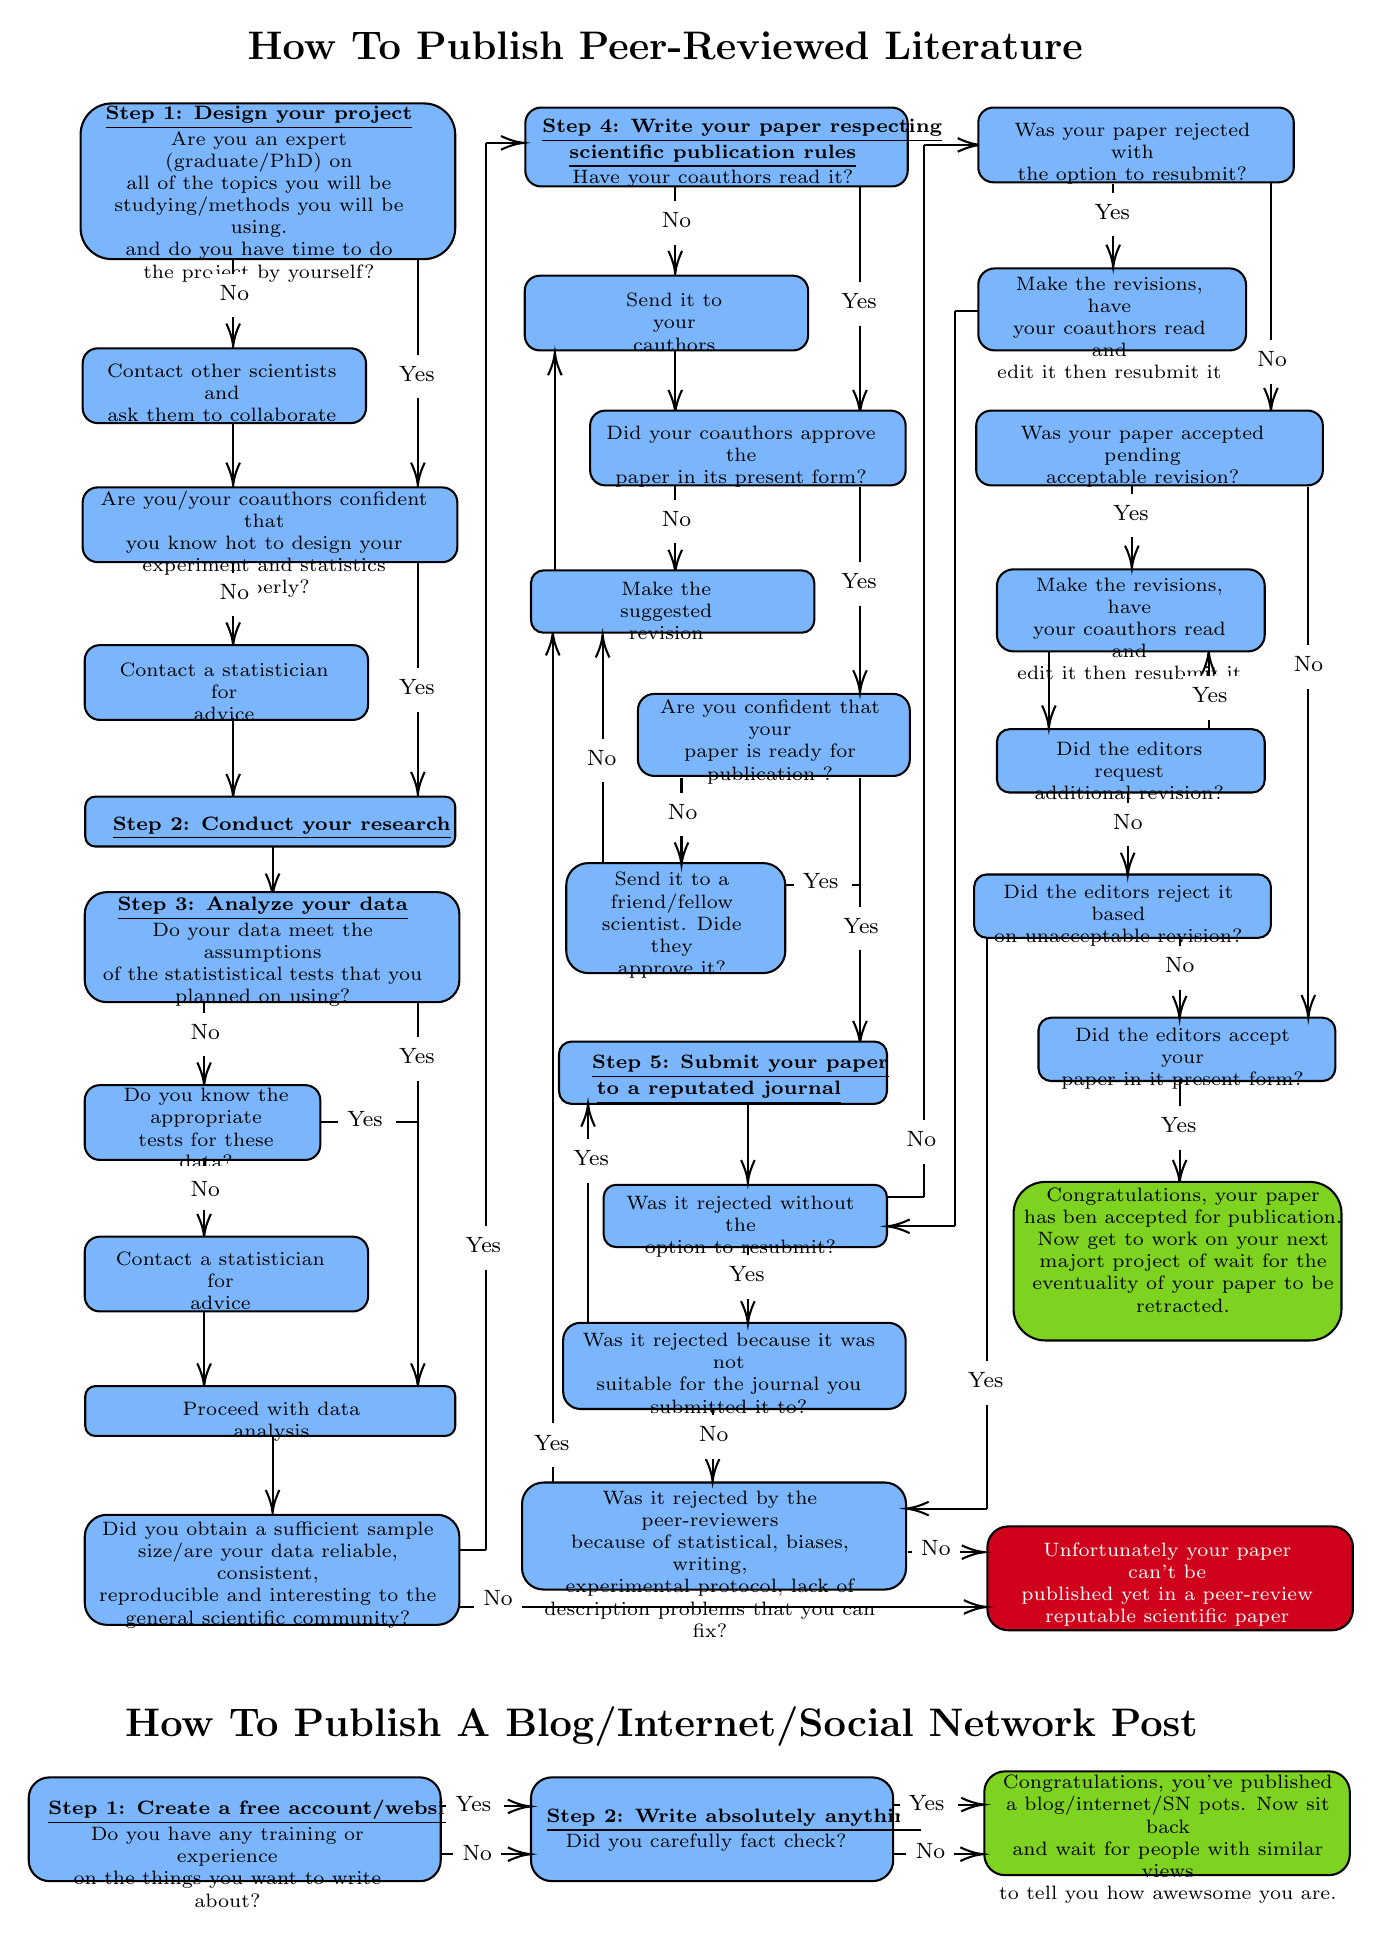
\begin{tikzpicture}[x=0.75pt,y=0.75pt,yscale=-1,xscale=1]
		%uncomment if require: \path (0,1077); %set diagram left start at 0, and has height of 1077
		
		%Straight Lines [id:da7459141170220505] 
		\draw    (463.5,143) -- (475.5,143) ;
		%Straight Lines [id:da13327973288575334] 
		\draw    (585.5,347) -- (585.5,309) ;
		\draw [shift={(585.5,307)}, rotate = 90] [color={rgb, 255:red, 0; green, 0; blue, 0 }  ][line width=0.75]    (10.93,-3.29) .. controls (6.95,-1.4) and (3.31,-0.3) .. (0,0) .. controls (3.31,0.3) and (6.95,1.4) .. (10.93,3.29)   ;
		%Straight Lines [id:da06946511985643378] 
		\draw    (615.5,81) -- (615.5,189) ;
		\draw [shift={(615.5,191)}, rotate = 270] [color={rgb, 255:red, 0; green, 0; blue, 0 }  ][line width=0.75]    (10.93,-3.29) .. controls (6.95,-1.4) and (3.31,-0.3) .. (0,0) .. controls (3.31,0.3) and (6.95,1.4) .. (10.93,3.29)   ;
		%Straight Lines [id:da26483183301153623] 
		\draw    (381.5,419.6) -- (417.5,419.6) ;
		%Straight Lines [id:da8358801252491679] 
		\draw    (269.5,707) -- (269.5,300) ;
		\draw [shift={(269.5,298)}, rotate = 90] [color={rgb, 255:red, 0; green, 0; blue, 0 }  ][line width=0.75]    (10.93,-3.29) .. controls (6.95,-1.4) and (3.31,-0.3) .. (0,0) .. controls (3.31,0.3) and (6.95,1.4) .. (10.93,3.29)   ;
		%Straight Lines [id:da28134647246307654] 
		\draw    (448.5,63) -- (473.5,63) ;
		\draw [shift={(475.5,63)}, rotate = 180] [color={rgb, 255:red, 0; green, 0; blue, 0 }  ][line width=0.75]    (10.93,-3.29) .. controls (6.95,-1.4) and (3.31,-0.3) .. (0,0) .. controls (3.31,0.3) and (6.95,1.4) .. (10.93,3.29)   ;
		%Straight Lines [id:da12619404453525518] 
		\draw    (204.5,476) -- (204.5,659) ;
		\draw [shift={(204.5,661)}, rotate = 270] [color={rgb, 255:red, 0; green, 0; blue, 0 }  ][line width=0.75]    (10.93,-3.29) .. controls (6.95,-1.4) and (3.31,-0.3) .. (0,0) .. controls (3.31,0.3) and (6.95,1.4) .. (10.93,3.29)   ;
		%Straight Lines [id:da547645088629442] 
		\draw    (101.5,624) -- (101.5,659) ;
		\draw [shift={(101.5,661)}, rotate = 270] [color={rgb, 255:red, 0; green, 0; blue, 0 }  ][line width=0.75]    (10.93,-3.29) .. controls (6.95,-1.4) and (3.31,-0.3) .. (0,0) .. controls (3.31,0.3) and (6.95,1.4) .. (10.93,3.29)   ;
		%Rounded Rect [id:dp5212760337767703] 
		\draw  [fill={rgb, 255:red, 123; green, 182; blue, 252 }  ,fill opacity=1 ] (42,58) .. controls (42,49.72) and (48.72,43) .. (57,43) -- (207.5,43) .. controls (215.78,43) and (222.5,49.72) .. (222.5,58) -- (222.5,103) .. controls (222.5,111.28) and (215.78,118) .. (207.5,118) -- (57,118) .. controls (48.72,118) and (42,111.28) .. (42,103) -- cycle ;
		%Straight Lines [id:da1071639108206357] 
		\draw    (115.5,118) -- (115.5,158) ;
		\draw [shift={(115.5,160)}, rotate = 270] [color={rgb, 255:red, 0; green, 0; blue, 0 }  ][line width=0.75]    (10.93,-3.29) .. controls (6.95,-1.4) and (3.31,-0.3) .. (0,0) .. controls (3.31,0.3) and (6.95,1.4) .. (10.93,3.29)   ;
		%Rounded Rect [id:dp23109480137264815] 
		\draw  [fill={rgb, 255:red, 123; green, 182; blue, 252 }  ,fill opacity=1 ] (43,168.2) .. controls (43,164.22) and (46.22,161) .. (50.2,161) -- (172.3,161) .. controls (176.28,161) and (179.5,164.22) .. (179.5,168.2) -- (179.5,189.8) .. controls (179.5,193.78) and (176.28,197) .. (172.3,197) -- (50.2,197) .. controls (46.22,197) and (43,193.78) .. (43,189.8) -- cycle ;
		%Straight Lines [id:da3457353493689892] 
		\draw    (115.5,197) -- (115.5,225) ;
		\draw [shift={(115.5,227)}, rotate = 270] [color={rgb, 255:red, 0; green, 0; blue, 0 }  ][line width=0.75]    (10.93,-3.29) .. controls (6.95,-1.4) and (3.31,-0.3) .. (0,0) .. controls (3.31,0.3) and (6.95,1.4) .. (10.93,3.29)   ;
		%Straight Lines [id:da493182538382704] 
		\draw    (204.5,118) -- (204.5,225) ;
		\draw [shift={(204.5,227)}, rotate = 270] [color={rgb, 255:red, 0; green, 0; blue, 0 }  ][line width=0.75]    (10.93,-3.29) .. controls (6.95,-1.4) and (3.31,-0.3) .. (0,0) .. controls (3.31,0.3) and (6.95,1.4) .. (10.93,3.29)   ;
		%Rounded Rect [id:dp04164017047600188] 
		\draw  [fill={rgb, 255:red, 123; green, 182; blue, 252 }  ,fill opacity=1 ] (43,235.2) .. controls (43,231.22) and (46.22,228) .. (50.2,228) -- (216.3,228) .. controls (220.28,228) and (223.5,231.22) .. (223.5,235.2) -- (223.5,256.8) .. controls (223.5,260.78) and (220.28,264) .. (216.3,264) -- (50.2,264) .. controls (46.22,264) and (43,260.78) .. (43,256.8) -- cycle ;
		%Straight Lines [id:da5877955095784488] 
		\draw    (115.5,264) -- (115.5,302) ;
		\draw [shift={(115.5,304)}, rotate = 270] [color={rgb, 255:red, 0; green, 0; blue, 0 }  ][line width=0.75]    (10.93,-3.29) .. controls (6.95,-1.4) and (3.31,-0.3) .. (0,0) .. controls (3.31,0.3) and (6.95,1.4) .. (10.93,3.29)   ;
		%Rounded Rect [id:dp061453494411897625] 
		\draw  [fill={rgb, 255:red, 123; green, 182; blue, 252 }  ,fill opacity=1 ] (44,311.2) .. controls (44,307.22) and (47.22,304) .. (51.2,304) -- (173.3,304) .. controls (177.28,304) and (180.5,307.22) .. (180.5,311.2) -- (180.5,332.8) .. controls (180.5,336.78) and (177.28,340) .. (173.3,340) -- (51.2,340) .. controls (47.22,340) and (44,336.78) .. (44,332.8) -- cycle ;
		%Straight Lines [id:da21553743104213607] 
		\draw    (204.5,264) -- (204.5,374) ;
		\draw [shift={(204.5,376)}, rotate = 270] [color={rgb, 255:red, 0; green, 0; blue, 0 }  ][line width=0.75]    (10.93,-3.29) .. controls (6.95,-1.4) and (3.31,-0.3) .. (0,0) .. controls (3.31,0.3) and (6.95,1.4) .. (10.93,3.29)   ;
		%Straight Lines [id:da03247087101876733] 
		\draw    (115.5,339) -- (115.5,375) ;
		\draw [shift={(115.5,377)}, rotate = 270] [color={rgb, 255:red, 0; green, 0; blue, 0 }  ][line width=0.75]    (10.93,-3.29) .. controls (6.95,-1.4) and (3.31,-0.3) .. (0,0) .. controls (3.31,0.3) and (6.95,1.4) .. (10.93,3.29)   ;
		%Rounded Rect [id:dp5810110360434235] 
		\draw  [fill={rgb, 255:red, 123; green, 182; blue, 252 }  ,fill opacity=1 ] (44.25,381.8) .. controls (44.25,379.15) and (46.4,377) .. (49.05,377) -- (217.7,377) .. controls (220.35,377) and (222.5,379.15) .. (222.5,381.8) -- (222.5,396.2) .. controls (222.5,398.85) and (220.35,401) .. (217.7,401) -- (49.05,401) .. controls (46.4,401) and (44.25,398.85) .. (44.25,396.2) -- cycle ;
		%Straight Lines [id:da9048314289105241] 
		\draw    (134.5,401) -- (134.5,423) ;
		\draw [shift={(134.5,425)}, rotate = 270] [color={rgb, 255:red, 0; green, 0; blue, 0 }  ][line width=0.75]    (10.93,-3.29) .. controls (6.95,-1.4) and (3.31,-0.3) .. (0,0) .. controls (3.31,0.3) and (6.95,1.4) .. (10.93,3.29)   ;
		%Rounded Rect [id:dp7467186164972284] 
		\draw  [fill={rgb, 255:red, 123; green, 182; blue, 252 }  ,fill opacity=1 ] (44,433.6) .. controls (44,427.75) and (48.75,423) .. (54.6,423) -- (213.9,423) .. controls (219.75,423) and (224.5,427.75) .. (224.5,433.6) -- (224.5,465.4) .. controls (224.5,471.25) and (219.75,476) .. (213.9,476) -- (54.6,476) .. controls (48.75,476) and (44,471.25) .. (44,465.4) -- cycle ;
		%Straight Lines [id:da14075809202882295] 
		\draw    (101.5,476) -- (101.5,514) ;
		\draw [shift={(101.5,516)}, rotate = 270] [color={rgb, 255:red, 0; green, 0; blue, 0 }  ][line width=0.75]    (10.93,-3.29) .. controls (6.95,-1.4) and (3.31,-0.3) .. (0,0) .. controls (3.31,0.3) and (6.95,1.4) .. (10.93,3.29)   ;
		%Rounded Rect [id:dp35686563328315124] 
		\draw  [fill={rgb, 255:red, 123; green, 182; blue, 252 }  ,fill opacity=1 ] (44,523.2) .. controls (44,519.22) and (47.22,516) .. (51.2,516) -- (150.3,516) .. controls (154.28,516) and (157.5,519.22) .. (157.5,523.2) -- (157.5,544.8) .. controls (157.5,548.78) and (154.28,552) .. (150.3,552) -- (51.2,552) .. controls (47.22,552) and (44,548.78) .. (44,544.8) -- cycle ;
		%Straight Lines [id:da6359551967325625] 
		\draw    (101.5,551) -- (101.5,587) ;
		\draw [shift={(101.5,589)}, rotate = 270] [color={rgb, 255:red, 0; green, 0; blue, 0 }  ][line width=0.75]    (10.93,-3.29) .. controls (6.95,-1.4) and (3.31,-0.3) .. (0,0) .. controls (3.31,0.3) and (6.95,1.4) .. (10.93,3.29)   ;
		%Rounded Rect [id:dp5746138831845229] 
		\draw  [fill={rgb, 255:red, 123; green, 182; blue, 252 }  ,fill opacity=1 ] (44,596.2) .. controls (44,592.22) and (47.22,589) .. (51.2,589) -- (173.3,589) .. controls (177.28,589) and (180.5,592.22) .. (180.5,596.2) -- (180.5,617.8) .. controls (180.5,621.78) and (177.28,625) .. (173.3,625) -- (51.2,625) .. controls (47.22,625) and (44,621.78) .. (44,617.8) -- cycle ;
		%Straight Lines [id:da5689047017320894] 
		\draw    (157.5,533.8) -- (204.5,533.8) ;
		%Rounded Rect [id:dp42076681669121263] 
		\draw  [fill={rgb, 255:red, 123; green, 182; blue, 252 }  ,fill opacity=1 ] (44.25,665.8) .. controls (44.25,663.15) and (46.4,661) .. (49.05,661) -- (217.7,661) .. controls (220.35,661) and (222.5,663.15) .. (222.5,665.8) -- (222.5,680.2) .. controls (222.5,682.85) and (220.35,685) .. (217.7,685) -- (49.05,685) .. controls (46.4,685) and (44.25,682.85) .. (44.25,680.2) -- cycle ;
		%Straight Lines [id:da5536212371550118] 
		\draw    (134.5,685) -- (134.5,720) ;
		\draw [shift={(134.5,722)}, rotate = 270] [color={rgb, 255:red, 0; green, 0; blue, 0 }  ][line width=0.75]    (10.93,-3.29) .. controls (6.95,-1.4) and (3.31,-0.3) .. (0,0) .. controls (3.31,0.3) and (6.95,1.4) .. (10.93,3.29)   ;
		%Rounded Rect [id:dp7669567378634832] 
		\draw  [fill={rgb, 255:red, 123; green, 182; blue, 252 }  ,fill opacity=1 ] (44,733.6) .. controls (44,727.75) and (48.75,723) .. (54.6,723) -- (213.9,723) .. controls (219.75,723) and (224.5,727.75) .. (224.5,733.6) -- (224.5,765.4) .. controls (224.5,771.25) and (219.75,776) .. (213.9,776) -- (54.6,776) .. controls (48.75,776) and (44,771.25) .. (44,765.4) -- cycle ;
		%Rounded Rect [id:dp700984008899528] 
		\draw  [fill={rgb, 255:red, 123; green, 182; blue, 252 }  ,fill opacity=1 ] (256.25,52.6) .. controls (256.25,48.4) and (259.65,45) .. (263.85,45) -- (432.9,45) .. controls (437.1,45) and (440.5,48.4) .. (440.5,52.6) -- (440.5,75.4) .. controls (440.5,79.6) and (437.1,83) .. (432.9,83) -- (263.85,83) .. controls (259.65,83) and (256.25,79.6) .. (256.25,75.4) -- cycle ;
		%Straight Lines [id:da24777567780381404] 
		\draw    (224.5,740) -- (237.5,740) ;
		%Straight Lines [id:da3240527161177258] 
		\draw    (237.5,740) -- (237.5,62) ;
		%Straight Lines [id:da11855638252992473] 
		\draw    (237.5,62) -- (253.5,62) ;
		\draw [shift={(255.5,62)}, rotate = 180] [color={rgb, 255:red, 0; green, 0; blue, 0 }  ][line width=0.75]    (10.93,-3.29) .. controls (6.95,-1.4) and (3.31,-0.3) .. (0,0) .. controls (3.31,0.3) and (6.95,1.4) .. (10.93,3.29)   ;
		%Straight Lines [id:da5437351912475403] 
		\draw    (328.5,83) -- (328.5,123) ;
		\draw [shift={(328.5,125)}, rotate = 270] [color={rgb, 255:red, 0; green, 0; blue, 0 }  ][line width=0.75]    (10.93,-3.29) .. controls (6.95,-1.4) and (3.31,-0.3) .. (0,0) .. controls (3.31,0.3) and (6.95,1.4) .. (10.93,3.29)   ;
		%Rounded Rect [id:dp10401634619407507] 
		\draw  [fill={rgb, 255:red, 123; green, 182; blue, 252 }  ,fill opacity=1 ] (256,133.2) .. controls (256,129.22) and (259.22,126) .. (263.2,126) -- (385.3,126) .. controls (389.28,126) and (392.5,129.22) .. (392.5,133.2) -- (392.5,154.8) .. controls (392.5,158.78) and (389.28,162) .. (385.3,162) -- (263.2,162) .. controls (259.22,162) and (256,158.78) .. (256,154.8) -- cycle ;
		%Straight Lines [id:da7863820012479865] 
		\draw    (328.5,162) -- (328.5,190) ;
		\draw [shift={(328.5,192)}, rotate = 270] [color={rgb, 255:red, 0; green, 0; blue, 0 }  ][line width=0.75]    (10.93,-3.29) .. controls (6.95,-1.4) and (3.31,-0.3) .. (0,0) .. controls (3.31,0.3) and (6.95,1.4) .. (10.93,3.29)   ;
		%Straight Lines [id:da6246637460301039] 
		\draw    (417.5,83) -- (417.5,190) ;
		\draw [shift={(417.5,192)}, rotate = 270] [color={rgb, 255:red, 0; green, 0; blue, 0 }  ][line width=0.75]    (10.93,-3.29) .. controls (6.95,-1.4) and (3.31,-0.3) .. (0,0) .. controls (3.31,0.3) and (6.95,1.4) .. (10.93,3.29)   ;
		%Rounded Rect [id:dp24564595256703514] 
		\draw  [fill={rgb, 255:red, 123; green, 182; blue, 252 }  ,fill opacity=1 ] (287.5,198.2) .. controls (287.5,194.22) and (290.72,191) .. (294.7,191) -- (432.3,191) .. controls (436.28,191) and (439.5,194.22) .. (439.5,198.2) -- (439.5,219.8) .. controls (439.5,223.78) and (436.28,227) .. (432.3,227) -- (294.7,227) .. controls (290.72,227) and (287.5,223.78) .. (287.5,219.8) -- cycle ;
		%Straight Lines [id:da888707123102463] 
		\draw    (328.5,227) -- (328.5,267) ;
		\draw [shift={(328.5,269)}, rotate = 270] [color={rgb, 255:red, 0; green, 0; blue, 0 }  ][line width=0.75]    (10.93,-3.29) .. controls (6.95,-1.4) and (3.31,-0.3) .. (0,0) .. controls (3.31,0.3) and (6.95,1.4) .. (10.93,3.29)   ;
		%Rounded Rect [id:dp09490195607934959] 
		\draw  [fill={rgb, 255:red, 123; green, 182; blue, 252 }  ,fill opacity=1 ] (259,274) .. controls (259,270.69) and (261.69,268) .. (265,268) -- (389.5,268) .. controls (392.81,268) and (395.5,270.69) .. (395.5,274) -- (395.5,292) .. controls (395.5,295.31) and (392.81,298) .. (389.5,298) -- (265,298) .. controls (261.69,298) and (259,295.31) .. (259,292) -- cycle ;
		%Straight Lines [id:da06910615271315823] 
		\draw    (270.5,268) -- (270.5,165) ;
		\draw [shift={(270.5,163)}, rotate = 90] [color={rgb, 255:red, 0; green, 0; blue, 0 }  ][line width=0.75]    (10.93,-3.29) .. controls (6.95,-1.4) and (3.31,-0.3) .. (0,0) .. controls (3.31,0.3) and (6.95,1.4) .. (10.93,3.29)   ;
		%Rounded Rect [id:dp1297606157343032] 
		\draw  [fill={rgb, 255:red, 123; green, 182; blue, 252 }  ,fill opacity=1 ] (17,859.5) .. controls (17,853.98) and (21.48,849.5) .. (27,849.5) -- (205.5,849.5) .. controls (211.02,849.5) and (215.5,853.98) .. (215.5,859.5) -- (215.5,889.5) .. controls (215.5,895.02) and (211.02,899.5) .. (205.5,899.5) -- (27,899.5) .. controls (21.48,899.5) and (17,895.02) .. (17,889.5) -- cycle ;
		%Rounded Rect [id:dp4783802338604324] 
		\draw  [fill={rgb, 255:red, 123; green, 182; blue, 252 }  ,fill opacity=1 ] (259,859.5) .. controls (259,853.98) and (263.48,849.5) .. (269,849.5) -- (423.5,849.5) .. controls (429.02,849.5) and (433.5,853.98) .. (433.5,859.5) -- (433.5,889.5) .. controls (433.5,895.02) and (429.02,899.5) .. (423.5,899.5) -- (269,899.5) .. controls (263.48,899.5) and (259,895.02) .. (259,889.5) -- cycle ;
		%Straight Lines [id:da33668612862785485] 
		\draw    (215.5,863.5) -- (256.8,863.5) ;
		\draw [shift={(258.8,863.5)}, rotate = 180] [color={rgb, 255:red, 0; green, 0; blue, 0 }  ][line width=0.75]    (10.93,-3.29) .. controls (6.95,-1.4) and (3.31,-0.3) .. (0,0) .. controls (3.31,0.3) and (6.95,1.4) .. (10.93,3.29)   ;
		%Rounded Rect [id:dp7694466613202249] 
		\draw  [fill={rgb, 255:red, 126; green, 211; blue, 33 }  ,fill opacity=1 ] (477.4,856.6) .. controls (477.4,851.08) and (481.88,846.6) .. (487.4,846.6) -- (643.5,846.6) .. controls (649.02,846.6) and (653.5,851.08) .. (653.5,856.6) -- (653.5,886.6) .. controls (653.5,892.12) and (649.02,896.6) .. (643.5,896.6) -- (487.4,896.6) .. controls (481.88,896.6) and (477.4,892.12) .. (477.4,886.6) -- cycle ;
		%Straight Lines [id:da8673762257073543] 
		\draw    (433.9,862.6) -- (475.2,862.6) ;
		\draw [shift={(477.2,862.6)}, rotate = 180] [color={rgb, 255:red, 0; green, 0; blue, 0 }  ][line width=0.75]    (10.93,-3.29) .. controls (6.95,-1.4) and (3.31,-0.3) .. (0,0) .. controls (3.31,0.3) and (6.95,1.4) .. (10.93,3.29)   ;
		%Rounded Rect [id:dp6285322628193803] 
		\draw  [fill={rgb, 255:red, 123; green, 182; blue, 252 }  ,fill opacity=1 ] (310.5,335.39) .. controls (310.5,331.03) and (314.04,327.49) .. (318.4,327.49) -- (433.6,327.49) .. controls (437.96,327.49) and (441.5,331.03) .. (441.5,335.39) -- (441.5,359.1) .. controls (441.5,363.46) and (437.96,367) .. (433.6,367) -- (318.4,367) .. controls (314.04,367) and (310.5,363.46) .. (310.5,359.1) -- cycle ;
		%Straight Lines [id:da1765410854051821] 
		\draw    (417.5,228) -- (417.5,325) ;
		\draw [shift={(417.5,327)}, rotate = 270] [color={rgb, 255:red, 0; green, 0; blue, 0 }  ][line width=0.75]    (10.93,-3.29) .. controls (6.95,-1.4) and (3.31,-0.3) .. (0,0) .. controls (3.31,0.3) and (6.95,1.4) .. (10.93,3.29)   ;
		%Rounded Rect [id:dp08473350304914229] 
		\draw  [fill={rgb, 255:red, 123; green, 182; blue, 252 }  ,fill opacity=1 ] (276,419.6) .. controls (276,413.75) and (280.75,409) .. (286.6,409) -- (370.9,409) .. controls (376.75,409) and (381.5,413.75) .. (381.5,419.6) -- (381.5,451.4) .. controls (381.5,457.25) and (376.75,462) .. (370.9,462) -- (286.6,462) .. controls (280.75,462) and (276,457.25) .. (276,451.4) -- cycle ;
		%Straight Lines [id:da525703446384703] 
		\draw    (331.5,368) -- (331.5,408) ;
		\draw [shift={(331.5,410)}, rotate = 270] [color={rgb, 255:red, 0; green, 0; blue, 0 }  ][line width=0.75]    (10.93,-3.29) .. controls (6.95,-1.4) and (3.31,-0.3) .. (0,0) .. controls (3.31,0.3) and (6.95,1.4) .. (10.93,3.29)   ;
		%Straight Lines [id:da7021653871438907] 
		\draw    (293.5,409) -- (293.5,301) ;
		\draw [shift={(293.5,299)}, rotate = 90] [color={rgb, 255:red, 0; green, 0; blue, 0 }  ][line width=0.75]    (10.93,-3.29) .. controls (6.95,-1.4) and (3.31,-0.3) .. (0,0) .. controls (3.31,0.3) and (6.95,1.4) .. (10.93,3.29)   ;
		%Straight Lines [id:da898404208893606] 
		\draw    (417.5,368) -- (417.5,494) ;
		\draw [shift={(417.5,496)}, rotate = 270] [color={rgb, 255:red, 0; green, 0; blue, 0 }  ][line width=0.75]    (10.93,-3.29) .. controls (6.95,-1.4) and (3.31,-0.3) .. (0,0) .. controls (3.31,0.3) and (6.95,1.4) .. (10.93,3.29)   ;
		%Rounded Rect [id:dp48551645159456536] 
		\draw  [fill={rgb, 255:red, 123; green, 182; blue, 252 }  ,fill opacity=1 ] (272.5,501) .. controls (272.5,497.69) and (275.19,495) .. (278.5,495) -- (424.5,495) .. controls (427.81,495) and (430.5,497.69) .. (430.5,501) -- (430.5,519) .. controls (430.5,522.31) and (427.81,525) .. (424.5,525) -- (278.5,525) .. controls (275.19,525) and (272.5,522.31) .. (272.5,519) -- cycle ;
		%Rounded Rect [id:dp7215594179357356] 
		\draw  [fill={rgb, 255:red, 123; green, 182; blue, 252 }  ,fill opacity=1 ] (294,570) .. controls (294,566.69) and (296.69,564) .. (300,564) -- (424.5,564) .. controls (427.81,564) and (430.5,566.69) .. (430.5,570) -- (430.5,588) .. controls (430.5,591.31) and (427.81,594) .. (424.5,594) -- (300,594) .. controls (296.69,594) and (294,591.31) .. (294,588) -- cycle ;
		%Straight Lines [id:da4874551979154209] 
		\draw    (363.5,524) -- (363.5,561) ;
		\draw [shift={(363.5,563)}, rotate = 270] [color={rgb, 255:red, 0; green, 0; blue, 0 }  ][line width=0.75]    (10.93,-3.29) .. controls (6.95,-1.4) and (3.31,-0.3) .. (0,0) .. controls (3.31,0.3) and (6.95,1.4) .. (10.93,3.29)   ;
		%Rounded Rect [id:dp10790295053471932] 
		\draw  [fill={rgb, 255:red, 123; green, 182; blue, 252 }  ,fill opacity=1 ] (274.5,638.79) .. controls (274.5,634.21) and (278.22,630.49) .. (282.8,630.49) -- (431.2,630.49) .. controls (435.78,630.49) and (439.5,634.21) .. (439.5,638.79) -- (439.5,663.7) .. controls (439.5,668.28) and (435.78,672) .. (431.2,672) -- (282.8,672) .. controls (278.22,672) and (274.5,668.28) .. (274.5,663.7) -- cycle ;
		%Straight Lines [id:da21983417540566608] 
		\draw    (363.5,594) -- (363.5,629) ;
		\draw [shift={(363.5,631)}, rotate = 270] [color={rgb, 255:red, 0; green, 0; blue, 0 }  ][line width=0.75]    (10.93,-3.29) .. controls (6.95,-1.4) and (3.31,-0.3) .. (0,0) .. controls (3.31,0.3) and (6.95,1.4) .. (10.93,3.29)   ;
		%Straight Lines [id:da004732610820221694] 
		\draw    (286.5,631) -- (286.5,527) ;
		\draw [shift={(286.5,525)}, rotate = 90] [color={rgb, 255:red, 0; green, 0; blue, 0 }  ][line width=0.75]    (10.93,-3.29) .. controls (6.95,-1.4) and (3.31,-0.3) .. (0,0) .. controls (3.31,0.3) and (6.95,1.4) .. (10.93,3.29)   ;
		%Rounded Rect [id:dp5949764218054425] 
		\draw  [fill={rgb, 255:red, 123; green, 182; blue, 252 }  ,fill opacity=1 ] (254.69,717.75) .. controls (254.69,712.06) and (259.31,707.44) .. (265,707.44) -- (429.38,707.44) .. controls (435.07,707.44) and (439.69,712.06) .. (439.69,717.75) -- (439.69,748.69) .. controls (439.69,754.38) and (435.07,759) .. (429.38,759) -- (265,759) .. controls (259.31,759) and (254.69,754.38) .. (254.69,748.69) -- cycle ;
		%Straight Lines [id:da28186392210799505] 
		\draw    (346.5,672) -- (346.5,700) -- (346.5,705) ;
		\draw [shift={(346.5,707)}, rotate = 270] [color={rgb, 255:red, 0; green, 0; blue, 0 }  ][line width=0.75]    (10.93,-3.29) .. controls (6.95,-1.4) and (3.31,-0.3) .. (0,0) .. controls (3.31,0.3) and (6.95,1.4) .. (10.93,3.29)   ;
		%Rounded Rect [id:dp30046999660110574] 
		\draw  [fill={rgb, 255:red, 123; green, 182; blue, 252 }  ,fill opacity=1 ] (474.5,52.2) .. controls (474.5,48.22) and (477.72,45) .. (481.7,45) -- (619.3,45) .. controls (623.28,45) and (626.5,48.22) .. (626.5,52.2) -- (626.5,73.8) .. controls (626.5,77.78) and (623.28,81) .. (619.3,81) -- (481.7,81) .. controls (477.72,81) and (474.5,77.78) .. (474.5,73.8) -- cycle ;
		%Straight Lines [id:da07785851854379411] 
		\draw    (430.5,570) -- (448.5,570) ;
		%Straight Lines [id:da4333160390459043] 
		\draw    (448.5,570) -- (448.5,63) ;
		%Rounded Rect [id:dp5097554942450033] 
		\draw  [fill={rgb, 255:red, 123; green, 182; blue, 252 }  ,fill opacity=1 ] (474.5,130.39) .. controls (474.5,126.03) and (478.04,122.49) .. (482.4,122.49) -- (595.6,122.49) .. controls (599.96,122.49) and (603.5,126.03) .. (603.5,130.39) -- (603.5,154.1) .. controls (603.5,158.46) and (599.96,162) .. (595.6,162) -- (482.4,162) .. controls (478.04,162) and (474.5,158.46) .. (474.5,154.1) -- cycle ;
		%Straight Lines [id:da8336873457127534] 
		\draw    (539.5,82) -- (539.5,120) ;
		\draw [shift={(539.5,122)}, rotate = 270] [color={rgb, 255:red, 0; green, 0; blue, 0 }  ][line width=0.75]    (10.93,-3.29) .. controls (6.95,-1.4) and (3.31,-0.3) .. (0,0) .. controls (3.31,0.3) and (6.95,1.4) .. (10.93,3.29)   ;
		%Rounded Rect [id:dp6961184266954239] 
		\draw  [fill={rgb, 255:red, 123; green, 182; blue, 252 }  ,fill opacity=1 ] (473.5,198.2) .. controls (473.5,194.22) and (476.72,191) .. (480.7,191) -- (633.3,191) .. controls (637.28,191) and (640.5,194.22) .. (640.5,198.2) -- (640.5,219.8) .. controls (640.5,223.78) and (637.28,227) .. (633.3,227) -- (480.7,227) .. controls (476.72,227) and (473.5,223.78) .. (473.5,219.8) -- cycle ;
		%Rounded Rect [id:dp6607194097830111] 
		\draw  [fill={rgb, 255:red, 123; green, 182; blue, 252 }  ,fill opacity=1 ] (483.5,275.39) .. controls (483.5,271.03) and (487.04,267.49) .. (491.4,267.49) -- (604.6,267.49) .. controls (608.96,267.49) and (612.5,271.03) .. (612.5,275.39) -- (612.5,299.1) .. controls (612.5,303.46) and (608.96,307) .. (604.6,307) -- (491.4,307) .. controls (487.04,307) and (483.5,303.46) .. (483.5,299.1) -- cycle ;
		%Straight Lines [id:da31213916714159917] 
		\draw    (548.5,227) -- (548.5,265) ;
		\draw [shift={(548.5,267)}, rotate = 270] [color={rgb, 255:red, 0; green, 0; blue, 0 }  ][line width=0.75]    (10.93,-3.29) .. controls (6.95,-1.4) and (3.31,-0.3) .. (0,0) .. controls (3.31,0.3) and (6.95,1.4) .. (10.93,3.29)   ;
		%Rounded Rect [id:dp12889075058086696] 
		\draw  [fill={rgb, 255:red, 123; green, 182; blue, 252 }  ,fill opacity=1 ] (483.5,350.59) .. controls (483.5,347.22) and (486.23,344.49) .. (489.6,344.49) -- (606.4,344.49) .. controls (609.77,344.49) and (612.5,347.22) .. (612.5,350.59) -- (612.5,368.9) .. controls (612.5,372.27) and (609.77,375) .. (606.4,375) -- (489.6,375) .. controls (486.23,375) and (483.5,372.27) .. (483.5,368.9) -- cycle ;
		%Straight Lines [id:da564091506726528] 
		\draw    (508.5,307) -- (508.5,342) ;
		\draw [shift={(508.5,344)}, rotate = 270] [color={rgb, 255:red, 0; green, 0; blue, 0 }  ][line width=0.75]    (10.93,-3.29) .. controls (6.95,-1.4) and (3.31,-0.3) .. (0,0) .. controls (3.31,0.3) and (6.95,1.4) .. (10.93,3.29)   ;
		%Rounded Rect [id:dp9473460275246046] 
		\draw  [fill={rgb, 255:red, 123; green, 182; blue, 252 }  ,fill opacity=1 ] (472.5,420.59) .. controls (472.5,417.22) and (475.23,414.49) .. (478.6,414.49) -- (609.4,414.49) .. controls (612.77,414.49) and (615.5,417.22) .. (615.5,420.59) -- (615.5,438.9) .. controls (615.5,442.27) and (612.77,445) .. (609.4,445) -- (478.6,445) .. controls (475.23,445) and (472.5,442.27) .. (472.5,438.9) -- cycle ;
		%Straight Lines [id:da9477678687674025] 
		\draw    (546.5,375) -- (546.5,413) ;
		\draw [shift={(546.5,415)}, rotate = 270] [color={rgb, 255:red, 0; green, 0; blue, 0 }  ][line width=0.75]    (10.93,-3.29) .. controls (6.95,-1.4) and (3.31,-0.3) .. (0,0) .. controls (3.31,0.3) and (6.95,1.4) .. (10.93,3.29)   ;
		%Rounded Rect [id:dp6777798697964894] 
		\draw  [fill={rgb, 255:red, 123; green, 182; blue, 252 }  ,fill opacity=1 ] (503.5,489.59) .. controls (503.5,486.22) and (506.23,483.49) .. (509.6,483.49) -- (640.4,483.49) .. controls (643.77,483.49) and (646.5,486.22) .. (646.5,489.59) -- (646.5,507.9) .. controls (646.5,511.27) and (643.77,514) .. (640.4,514) -- (509.6,514) .. controls (506.23,514) and (503.5,511.27) .. (503.5,507.9) -- cycle ;
		%Straight Lines [id:da2050643265478107] 
		\draw    (571.5,444) -- (571.5,482) ;
		\draw [shift={(571.5,484)}, rotate = 270] [color={rgb, 255:red, 0; green, 0; blue, 0 }  ][line width=0.75]    (10.93,-3.29) .. controls (6.95,-1.4) and (3.31,-0.3) .. (0,0) .. controls (3.31,0.3) and (6.95,1.4) .. (10.93,3.29)   ;
		%Straight Lines [id:da08817679327680361] 
		\draw    (633.5,228) -- (633.5,481.49) ;
		\draw [shift={(633.5,483.49)}, rotate = 270] [color={rgb, 255:red, 0; green, 0; blue, 0 }  ][line width=0.75]    (10.93,-3.29) .. controls (6.95,-1.4) and (3.31,-0.3) .. (0,0) .. controls (3.31,0.3) and (6.95,1.4) .. (10.93,3.29)   ;
		%Straight Lines [id:da573694186764033] 
		\draw    (463.5,584) -- (463.5,143) ;
		%Straight Lines [id:da3463527528126673] 
		\draw    (463.5,584) -- (432.5,584) ;
		\draw [shift={(430.5,584)}, rotate = 360] [color={rgb, 255:red, 0; green, 0; blue, 0 }  ][line width=0.75]    (10.93,-3.29) .. controls (6.95,-1.4) and (3.31,-0.3) .. (0,0) .. controls (3.31,0.3) and (6.95,1.4) .. (10.93,3.29)   ;
		%Straight Lines [id:da8002523895567404] 
		\draw    (571.5,513) -- (571.5,561) ;
		\draw [shift={(571.5,563)}, rotate = 270] [color={rgb, 255:red, 0; green, 0; blue, 0 }  ][line width=0.75]    (10.93,-3.29) .. controls (6.95,-1.4) and (3.31,-0.3) .. (0,0) .. controls (3.31,0.3) and (6.95,1.4) .. (10.93,3.29)   ;
		%Rounded Rect [id:dp3704955375094494] 
		\draw  [fill={rgb, 255:red, 126; green, 211; blue, 33 }  ,fill opacity=1 ] (491.5,577.88) .. controls (491.5,569.44) and (498.34,562.6) .. (506.78,562.6) -- (634.22,562.6) .. controls (642.66,562.6) and (649.5,569.44) .. (649.5,577.88) -- (649.5,623.72) .. controls (649.5,632.16) and (642.66,639) .. (634.22,639) -- (506.78,639) .. controls (498.34,639) and (491.5,632.16) .. (491.5,623.72) -- cycle ;
		%Rounded Rect [id:dp2634504509398907] 
		\draw  [fill={rgb, 255:red, 208; green, 2; blue, 27 }  ,fill opacity=1 ] (478.9,738.6) .. controls (478.9,733.08) and (483.38,728.6) .. (488.9,728.6) -- (645,728.6) .. controls (650.52,728.6) and (655,733.08) .. (655,738.6) -- (655,768.6) .. controls (655,774.12) and (650.52,778.6) .. (645,778.6) -- (488.9,778.6) .. controls (483.38,778.6) and (478.9,774.12) .. (478.9,768.6) -- cycle ;
		%Straight Lines [id:da19594871916070478] 
		\draw    (440.5,741) -- (475.5,741) ;
		\draw [shift={(477.5,741)}, rotate = 180] [color={rgb, 255:red, 0; green, 0; blue, 0 }  ][line width=0.75]    (10.93,-3.29) .. controls (6.95,-1.4) and (3.31,-0.3) .. (0,0) .. controls (3.31,0.3) and (6.95,1.4) .. (10.93,3.29)   ;
		%Straight Lines [id:da5099979660009493] 
		\draw    (224.5,767.4) -- (476.5,767.4) ;
		\draw [shift={(478.5,767.4)}, rotate = 180] [color={rgb, 255:red, 0; green, 0; blue, 0 }  ][line width=0.75]    (10.93,-3.29) .. controls (6.95,-1.4) and (3.31,-0.3) .. (0,0) .. controls (3.31,0.3) and (6.95,1.4) .. (10.93,3.29)   ;
		%Straight Lines [id:da8756323773636032] 
		\draw    (478.6,445) -- (478.6,720) ;
		%Straight Lines [id:da8719817711308564] 
		\draw    (478.6,720) -- (441.69,720) ;
		\draw [shift={(439.69,720)}, rotate = 360] [color={rgb, 255:red, 0; green, 0; blue, 0 }  ][line width=0.75]    (10.93,-3.29) .. controls (6.95,-1.4) and (3.31,-0.3) .. (0,0) .. controls (3.31,0.3) and (6.95,1.4) .. (10.93,3.29)   ;
		%Straight Lines [id:da08169550838230588] 
		\draw    (215.5,886.5) -- (256.8,886.5) ;
		\draw [shift={(258.8,886.5)}, rotate = 180] [color={rgb, 255:red, 0; green, 0; blue, 0 }  ][line width=0.75]    (10.93,-3.29) .. controls (6.95,-1.4) and (3.31,-0.3) .. (0,0) .. controls (3.31,0.3) and (6.95,1.4) .. (10.93,3.29)   ;
		%Straight Lines [id:da8823774393351953] 
		\draw    (433.5,886.5) -- (474.8,886.5) ;
		\draw [shift={(476.8,886.5)}, rotate = 180] [color={rgb, 255:red, 0; green, 0; blue, 0 }  ][line width=0.75]    (10.93,-3.29) .. controls (6.95,-1.4) and (3.31,-0.3) .. (0,0) .. controls (3.31,0.3) and (6.95,1.4) .. (10.93,3.29)   ;
		
		% Text Node
		\draw (121,7) node [anchor=north west][inner sep=0.75pt]   [align=left] {\textbf{{\Large How To Publish Peer-Reviewed Literature}}};
		% Text Node
		\draw (45.25,43) node [anchor=north west][inner sep=0.75pt]  [font=\scriptsize] [align=left] {\begin{minipage}[lt]{121.79pt}\setlength\topsep{0pt}
		\begin{center}
		\underline{\textbf{Step 1: Design your project}}\\Are you an expert (graduate/PhD) on \\all of the topics you will be \\studying/methods you will be using.\\and do you have time to do\\the project by yourself?
		\end{center}
		
		\end{minipage}};
		% Text Node
		\draw  [draw opacity=0][fill={rgb, 255:red, 255; green, 255; blue, 255 }  ,fill opacity=1 ]  (104.5,125) -- (127.5,125) -- (127.5,146) -- (104.5,146) -- cycle  ;
		\draw (107.5,129) node [anchor=north west][inner sep=0.75pt]  [font=\footnotesize] [align=left] {No};
		% Text Node
		\draw (48,167) node [anchor=north west][inner sep=0.75pt]  [font=\scriptsize] [align=left] {\begin{minipage}[lt]{90.83pt}\setlength\topsep{0pt}
		\begin{center}
		Contact other scientists and\\ask them to collaborate
		\end{center}
		
		\end{minipage}};
		% Text Node
		\draw  [draw opacity=0][fill={rgb, 255:red, 255; green, 255; blue, 255 }  ,fill opacity=1 ]  (191,164) -- (219,164) -- (219,185) -- (191,185) -- cycle  ;
		\draw (194,168) node [anchor=north west][inner sep=0.75pt]  [font=\footnotesize] [align=left] {Yes};
		% Text Node
		\draw (48,228) node [anchor=north west][inner sep=0.75pt]  [font=\scriptsize] [align=left] {\begin{minipage}[lt]{121.4pt}\setlength\topsep{0pt}
		\begin{center}
		Are you/your coauthors confident that\\you know hot to design your\\experiment and statistics properly?
		\end{center}
		
		\end{minipage}};
		% Text Node
		\draw (57,311) node [anchor=north west][inner sep=0.75pt]  [font=\scriptsize] [align=left] {\begin{minipage}[lt]{78.92pt}\setlength\topsep{0pt}
		\begin{center}
		Contact a statistician for\\advice
		\end{center}
		
		\end{minipage}};
		% Text Node
		\draw  [draw opacity=0][fill={rgb, 255:red, 255; green, 255; blue, 255 }  ,fill opacity=1 ]  (104.5,269) -- (127.5,269) -- (127.5,290) -- (104.5,290) -- cycle  ;
		\draw (107.5,273) node [anchor=north west][inner sep=0.75pt]  [font=\footnotesize] [align=left] {No};
		% Text Node
		\draw  [draw opacity=0][fill={rgb, 255:red, 255; green, 255; blue, 255 }  ,fill opacity=1 ]  (191,315) -- (219,315) -- (219,336) -- (191,336) -- cycle  ;
		\draw (194,319) node [anchor=north west][inner sep=0.75pt]  [font=\footnotesize] [align=left] {Yes};
		% Text Node
		\draw (56,381) node [anchor=north west][inner sep=0.75pt]  [font=\scriptsize] [align=left] {\begin{minipage}[lt]{106.68pt}\setlength\topsep{0pt}
		\begin{center}
		\textbf{\underline{Step 2: Conduct your research}}
		\end{center}
		
		\end{minipage}};
		% Text Node
		\draw (51.25,424) node [anchor=north west][inner sep=0.75pt]  [font=\scriptsize] [align=left] {\begin{minipage}[lt]{115.44pt}\setlength\topsep{0pt}
		\begin{center}
		\underline{\textbf{Step 3: Analyze your data}}\\Do your data meet the assumptions\\of the statististical tests that you\\planned on using?
		\end{center}
		
		\end{minipage}};
		% Text Node
		\draw (56,516) node [anchor=north west][inner sep=0.75pt]  [font=\scriptsize] [align=left] {\begin{minipage}[lt]{67.43pt}\setlength\topsep{0pt}
		\begin{center}
		Do you know the \\appropriate\\tests for these data?
		\end{center}
		
		\end{minipage}};
		% Text Node
		\draw  [draw opacity=0][fill={rgb, 255:red, 255; green, 255; blue, 255 }  ,fill opacity=1 ]  (90.5,481) -- (113.5,481) -- (113.5,502) -- (90.5,502) -- cycle  ;
		\draw (93.5,485) node [anchor=north west][inner sep=0.75pt]  [font=\footnotesize] [align=left] {No};
		% Text Node
		\draw  [draw opacity=0][fill={rgb, 255:red, 255; green, 255; blue, 255 }  ,fill opacity=1 ]  (166,523) -- (194,523) -- (194,544) -- (166,544) -- cycle  ;
		\draw (169,527) node [anchor=north west][inner sep=0.75pt]  [font=\footnotesize] [align=left] {Yes};
		% Text Node
		\draw  [draw opacity=0][fill={rgb, 255:red, 255; green, 255; blue, 255 }  ,fill opacity=1 ]  (90.5,555) -- (113.5,555) -- (113.5,576) -- (90.5,576) -- cycle  ;
		\draw (93.5,561) node [anchor=north west][inner sep=0.75pt]  [font=\footnotesize] [align=left] {No};
		% Text Node
		\draw (55.25,595) node [anchor=north west][inner sep=0.75pt]  [font=\scriptsize] [align=left] {\begin{minipage}[lt]{78.92pt}\setlength\topsep{0pt}
		\begin{center}
		Contact a statistician for\\advice
		\end{center}
		
		\end{minipage}};
		% Text Node
		\draw  [draw opacity=0][fill={rgb, 255:red, 255; green, 255; blue, 255 }  ,fill opacity=1 ]  (191,493) -- (219,493) -- (219,514) -- (191,514) -- cycle  ;
		\draw (194,497) node [anchor=north west][inner sep=0.75pt]  [font=\footnotesize] [align=left] {Yes};
		% Text Node
		\draw (74,667) node [anchor=north west][inner sep=0.75pt]  [font=\scriptsize] [align=left] {\begin{minipage}[lt]{87.66pt}\setlength\topsep{0pt}
		\begin{center}
		Proceed with data analysis
		\end{center}
		
		\end{minipage}};
		% Text Node
		\draw (49,725) node [anchor=north west][inner sep=0.75pt]  [font=\scriptsize] [align=left] {\begin{minipage}[lt]{122.58pt}\setlength\topsep{0pt}
		\begin{center}
		Did you obtain a sufficient sample\\size/are your data reliable, consistent,\\reproducible and interesting to the \\general scientific community?
		\end{center}
		
		\end{minipage}};
		% Text Node
		\draw (263,45) node [anchor=north west][inner sep=0.75pt]  [font=\scriptsize] [align=left] {\begin{minipage}[lt]{123.21pt}\setlength\topsep{0pt}
		\begin{center}
		\textbf{\underline{Step 4: Write your paper respecting}}\\\underline{\textbf{scientific publication rules}}\\Have your coauthors read it?
		\end{center}
		
		\end{minipage}};
		% Text Node
		\draw  [draw opacity=0][fill={rgb, 255:red, 255; green, 255; blue, 255 }  ,fill opacity=1 ]  (223,584) -- (251,584) -- (251,605) -- (223,605) -- cycle  ;
		\draw (226,588) node [anchor=north west][inner sep=0.75pt]  [font=\footnotesize] [align=left] {Yes};
		% Text Node
		\draw  [draw opacity=0][fill={rgb, 255:red, 255; green, 255; blue, 255 }  ,fill opacity=1 ]  (317.5,90) -- (340.5,90) -- (340.5,111) -- (317.5,111) -- cycle  ;
		\draw (320.5,94) node [anchor=north west][inner sep=0.75pt]  [font=\footnotesize] [align=left] {No};
		% Text Node
		\draw (294,133) node [anchor=north west][inner sep=0.75pt]  [font=\scriptsize] [align=left] {\begin{minipage}[lt]{48.77pt}\setlength\topsep{0pt}
		\begin{center}
		Send it to your\\cauthors
		\end{center}
		
		\end{minipage}};
		% Text Node
		\draw  [draw opacity=0][fill={rgb, 255:red, 255; green, 255; blue, 255 }  ,fill opacity=1 ]  (404,129) -- (432,129) -- (432,150) -- (404,150) -- cycle  ;
		\draw (407,133) node [anchor=north west][inner sep=0.75pt]  [font=\footnotesize] [align=left] {Yes};
		% Text Node
		\draw (290.5,197) node [anchor=north west][inner sep=0.75pt]  [font=\scriptsize] [align=left] {\begin{minipage}[lt]{102.35pt}\setlength\topsep{0pt}
		\begin{center}
		Did your coauthors approve the\\paper in its present form?
		\end{center}
		
		\end{minipage}};
		% Text Node
		\draw  [draw opacity=0][fill={rgb, 255:red, 255; green, 255; blue, 255 }  ,fill opacity=1 ]  (317.5,234) -- (340.5,234) -- (340.5,255) -- (317.5,255) -- cycle  ;
		\draw (320.5,238) node [anchor=north west][inner sep=0.75pt]  [font=\footnotesize] [align=left] {No};
		% Text Node
		\draw (278,272) node [anchor=north west][inner sep=0.75pt]  [font=\scriptsize] [align=left] {\begin{minipage}[lt]{67.02pt}\setlength\topsep{0pt}
		\begin{center}
		Make the suggested\\revision
		\end{center}
		
		\end{minipage}};
		% Text Node
		\draw (62,814) node [anchor=north west][inner sep=0.75pt]   [align=left] {\textbf{{\Large How To Publish A Blog/Internet/Social Network Post}}};
		% Text Node
		\draw (25,855) node [anchor=north west][inner sep=0.75pt]  [font=\scriptsize] [align=left] {\begin{minipage}[lt]{129.31pt}\setlength\topsep{0pt}
		\begin{center}
		\underline{\textbf{Step 1: Create a free account/website}}\\Do you have any training or experience\\on the things you want to write about?
		\end{center}
		
		\end{minipage}};
		% Text Node
		\draw (265,859) node [anchor=north west][inner sep=0.75pt]  [font=\scriptsize] [align=left] {\begin{minipage}[lt]{115.26pt}\setlength\topsep{0pt}
		\begin{center}
		\underline{\textbf{Step 2: Write absolutely anything}}\\Did you carefully fact check?
		\end{center}
		
		\end{minipage}};
		% Text Node
		\draw  [draw opacity=0][fill={rgb, 255:red, 255; green, 255; blue, 255 }  ,fill opacity=1 ]  (221.5,877) -- (244.5,877) -- (244.5,898) -- (221.5,898) -- cycle  ;
		\draw (224.5,881) node [anchor=north west][inner sep=0.75pt]  [font=\footnotesize] [align=left] {No};
		% Text Node
		\draw  [draw opacity=0][fill={rgb, 255:red, 255; green, 255; blue, 255 }  ,fill opacity=1 ]  (218.2,853) -- (246.2,853) -- (246.2,874) -- (218.2,874) -- cycle  ;
		\draw (221.2,857) node [anchor=north west][inner sep=0.75pt]  [font=\footnotesize] [align=left] {Yes};
		% Text Node
		\draw (481,847) node [anchor=north west][inner sep=0.75pt]  [font=\scriptsize] [align=left] {\begin{minipage}[lt]{125pt}\setlength\topsep{0pt}
		\begin{center}
		Congratulations, you've published\\a blog/internet/SN pots. Now sit back\\and wait for people with similar views\\to tell you how awewsome you are.
		\end{center}
		
		\end{minipage}};
		% Text Node
		\draw  [draw opacity=0][fill={rgb, 255:red, 255; green, 255; blue, 255 }  ,fill opacity=1 ]  (439.9,875.6) -- (462.9,875.6) -- (462.9,896.6) -- (439.9,896.6) -- cycle  ;
		\draw (442.9,879.6) node [anchor=north west][inner sep=0.75pt]  [font=\footnotesize] [align=left] {No};
		% Text Node
		\draw  [draw opacity=0][fill={rgb, 255:red, 255; green, 255; blue, 255 }  ,fill opacity=1 ]  (436.6,852.6) -- (464.6,852.6) -- (464.6,873.6) -- (436.6,873.6) -- cycle  ;
		\draw (439.6,856.6) node [anchor=north west][inner sep=0.75pt]  [font=\footnotesize] [align=left] {Yes};
		% Text Node
		\draw (314,329) node [anchor=north west][inner sep=0.75pt]  [font=\scriptsize] [align=left] {\begin{minipage}[lt]{88.06pt}\setlength\topsep{0pt}
		\begin{center}
		Are you confident that your\\paper is ready for\\publication ?
		\end{center}
		
		\end{minipage}};
		% Text Node
		\draw  [draw opacity=0][fill={rgb, 255:red, 255; green, 255; blue, 255 }  ,fill opacity=1 ]  (404,264) -- (432,264) -- (432,285) -- (404,285) -- cycle  ;
		\draw (407,268) node [anchor=north west][inner sep=0.75pt]  [font=\footnotesize] [align=left] {Yes};
		% Text Node
		\draw (283.6,412) node [anchor=north west][inner sep=0.75pt]  [font=\scriptsize] [align=left] {\begin{minipage}[lt]{62.65pt}\setlength\topsep{0pt}
		\begin{center}
		Send it to a\\friend/fellow\\scientist. Dide they\\approve it?
		\end{center}
		
		\end{minipage}};
		% Text Node
		\draw  [draw opacity=0][fill={rgb, 255:red, 255; green, 255; blue, 255 }  ,fill opacity=1 ]  (320.5,375) -- (343.5,375) -- (343.5,396) -- (320.5,396) -- cycle  ;
		\draw (323.5,379) node [anchor=north west][inner sep=0.75pt]  [font=\footnotesize] [align=left] {No};
		% Text Node
		\draw  [draw opacity=0][fill={rgb, 255:red, 255; green, 255; blue, 255 }  ,fill opacity=1 ]  (281.5,349) -- (304.5,349) -- (304.5,370) -- (281.5,370) -- cycle  ;
		\draw (284.5,353) node [anchor=north west][inner sep=0.75pt]  [font=\footnotesize] [align=left] {No};
		% Text Node
		\draw  [draw opacity=0][fill={rgb, 255:red, 255; green, 255; blue, 255 }  ,fill opacity=1 ]  (405,430) -- (433,430) -- (433,451) -- (405,451) -- cycle  ;
		\draw (408,434) node [anchor=north west][inner sep=0.75pt]  [font=\footnotesize] [align=left] {Yes};
		% Text Node
		\draw (287,496) node [anchor=north west][inner sep=0.75pt]  [font=\scriptsize] [align=left] {\begin{minipage}[lt]{91.59pt}\setlength\topsep{0pt}
		\begin{center}
		\textbf{\underline{Step 5: Submit your paper}}\\\textbf{\underline{to a reputated journal}}
		\end{center}
		
		\end{minipage}};
		% Text Node
		\draw  [draw opacity=0][fill={rgb, 255:red, 255; green, 255; blue, 255 }  ,fill opacity=1 ]  (385.5,408.4) -- (413.5,408.4) -- (413.5,429.4) -- (385.5,429.4) -- cycle  ;
		\draw (388.5,412.4) node [anchor=north west][inner sep=0.75pt]  [font=\footnotesize] [align=left] {Yes};
		% Text Node
		\draw (301,568) node [anchor=north west][inner sep=0.75pt]  [font=\scriptsize] [align=left] {\begin{minipage}[lt]{86.19pt}\setlength\topsep{0pt}
		\begin{center}
		Was it rejected without the\\option to resubmit?
		\end{center}
		
		\end{minipage}};
		% Text Node
		\draw (279,634) node [anchor=north west][inner sep=0.75pt]  [font=\scriptsize] [align=left] {\begin{minipage}[lt]{110.8pt}\setlength\topsep{0pt}
		\begin{center}
		Was it rejected because it was not\\suitable for the journal you\\submitted it to?
		\end{center}
		
		\end{minipage}};
		% Text Node
		\draw  [draw opacity=0][fill={rgb, 255:red, 255; green, 255; blue, 255 }  ,fill opacity=1 ]  (350,598) -- (378,598) -- (378,619) -- (350,619) -- cycle  ;
		\draw (353,602) node [anchor=north west][inner sep=0.75pt]  [font=\footnotesize] [align=left] {Yes};
		% Text Node
		\draw  [draw opacity=0][fill={rgb, 255:red, 255; green, 255; blue, 255 }  ,fill opacity=1 ]  (275,542) -- (303,542) -- (303,563) -- (275,563) -- cycle  ;
		\draw (278,546) node [anchor=north west][inner sep=0.75pt]  [font=\footnotesize] [align=left] {Yes};
		% Text Node
		\draw (262,710) node [anchor=north west][inner sep=0.75pt]  [font=\scriptsize] [align=left] {\begin{minipage}[lt]{122.58pt}\setlength\topsep{0pt}
		\begin{center}
		Was it rejected by the peer-reviewers\\because of statistical, biases, writing, \\experimental protocol, lack of \\description problems that you can fix?
		\end{center}
		
		\end{minipage}};
		% Text Node
		\draw  [draw opacity=0][fill={rgb, 255:red, 255; green, 255; blue, 255 }  ,fill opacity=1 ]  (335.5,675) -- (358.5,675) -- (358.5,696) -- (335.5,696) -- cycle  ;
		\draw (338.5,679) node [anchor=north west][inner sep=0.75pt]  [font=\footnotesize] [align=left] {No};
		% Text Node
		\draw  [draw opacity=0][fill={rgb, 255:red, 255; green, 255; blue, 255 }  ,fill opacity=1 ]  (256,679) -- (284,679) -- (284,700) -- (256,700) -- cycle  ;
		\draw (259,683) node [anchor=north west][inner sep=0.75pt]  [font=\footnotesize] [align=left] {Yes};
		% Text Node
		\draw (484,51) node [anchor=north west][inner sep=0.75pt]  [font=\scriptsize] [align=left] {\begin{minipage}[lt]{94.92pt}\setlength\topsep{0pt}
		\begin{center}
		Was your paper rejected with\\the option to resubmit?
		\end{center}
		
		\end{minipage}};
		% Text Node
		\draw  [draw opacity=0][fill={rgb, 255:red, 255; green, 255; blue, 255 }  ,fill opacity=1 ]  (435.5,533) -- (458.5,533) -- (458.5,554) -- (435.5,554) -- cycle  ;
		\draw (438.5,537) node [anchor=north west][inner sep=0.75pt]  [font=\footnotesize] [align=left] {No};
		% Text Node
		\draw (480.4,125) node [anchor=north west][inner sep=0.75pt]  [font=\scriptsize] [align=left] {\begin{minipage}[lt]{83.68pt}\setlength\topsep{0pt}
		\begin{center}
		Make the revisions, have \\your coauthors read and \\edit it then resubmit it
		\end{center}
		
		\end{minipage}};
		% Text Node
		\draw  [draw opacity=0][fill={rgb, 255:red, 255; green, 255; blue, 255 }  ,fill opacity=1 ]  (526,86) -- (554,86) -- (554,107) -- (526,107) -- cycle  ;
		\draw (529,90) node [anchor=north west][inner sep=0.75pt]  [font=\footnotesize] [align=left] {Yes};
		% Text Node
		\draw (478,197) node [anchor=north west][inner sep=0.75pt]  [font=\scriptsize] [align=left] {\begin{minipage}[lt]{111.21pt}\setlength\topsep{0pt}
		\begin{center}
		Was your paper accepted pending\\acceptable revision?
		\end{center}
		
		\end{minipage}};
		% Text Node
		\draw  [draw opacity=0][fill={rgb, 255:red, 255; green, 255; blue, 255 }  ,fill opacity=1 ]  (604.5,157) -- (627.5,157) -- (627.5,178) -- (604.5,178) -- cycle  ;
		\draw (607.5,161) node [anchor=north west][inner sep=0.75pt]  [font=\footnotesize] [align=left] {No};
		% Text Node
		\draw (490,270) node [anchor=north west][inner sep=0.75pt]  [font=\scriptsize] [align=left] {\begin{minipage}[lt]{83.68pt}\setlength\topsep{0pt}
		\begin{center}
		Make the revisions, have \\your coauthors read and \\edit it then resubmit it
		\end{center}
		
		\end{minipage}};
		% Text Node
		\draw  [draw opacity=0][fill={rgb, 255:red, 255; green, 255; blue, 255 }  ,fill opacity=1 ]  (535,231) -- (563,231) -- (563,252) -- (535,252) -- cycle  ;
		\draw (538,235) node [anchor=north west][inner sep=0.75pt]  [font=\footnotesize] [align=left] {Yes};
		% Text Node
		\draw (496,349) node [anchor=north west][inner sep=0.75pt]  [font=\scriptsize] [align=left] {\begin{minipage}[lt]{74.57pt}\setlength\topsep{0pt}
		\begin{center}
		Did the editors request\\additional revision?
		\end{center}
		
		\end{minipage}};
		% Text Node
		\draw  [draw opacity=0][fill={rgb, 255:red, 255; green, 255; blue, 255 }  ,fill opacity=1 ]  (573,319) -- (601,319) -- (601,340) -- (573,340) -- cycle  ;
		\draw (576,323) node [anchor=north west][inner sep=0.75pt]  [font=\footnotesize] [align=left] {Yes};
		% Text Node
		\draw (477,418) node [anchor=north west][inner sep=0.75pt]  [font=\scriptsize] [align=left] {\begin{minipage}[lt]{95.2pt}\setlength\topsep{0pt}
		\begin{center}
		Did the editors reject it based\\on unacceptable revision?
		\end{center}
		
		\end{minipage}};
		% Text Node
		\draw  [draw opacity=0][fill={rgb, 255:red, 255; green, 255; blue, 255 }  ,fill opacity=1 ]  (535,380) -- (558,380) -- (558,401) -- (535,401) -- cycle  ;
		\draw (538,384) node [anchor=north west][inner sep=0.75pt]  [font=\footnotesize] [align=left] {No};
		% Text Node
		\draw (513,487) node [anchor=north west][inner sep=0.75pt]  [font=\scriptsize] [align=left] {\begin{minipage}[lt]{87.66pt}\setlength\topsep{0pt}
		\begin{center}
		Did the editors accept your\\paper in it present form?
		\end{center}
		
		\end{minipage}};
		% Text Node
		\draw  [draw opacity=0][fill={rgb, 255:red, 255; green, 255; blue, 255 }  ,fill opacity=1 ]  (560,449) -- (583,449) -- (583,470) -- (560,470) -- cycle  ;
		\draw (563,453) node [anchor=north west][inner sep=0.75pt]  [font=\footnotesize] [align=left] {No};
		% Text Node
		\draw  [draw opacity=0][fill={rgb, 255:red, 255; green, 255; blue, 255 }  ,fill opacity=1 ]  (622,304) -- (645,304) -- (645,325) -- (622,325) -- cycle  ;
		\draw (625,308) node [anchor=north west][inner sep=0.75pt]  [font=\footnotesize] [align=left] {No};
		% Text Node
		\draw  [draw opacity=0][fill={rgb, 255:red, 255; green, 255; blue, 255 }  ,fill opacity=1 ]  (558,526) -- (586,526) -- (586,547) -- (558,547) -- cycle  ;
		\draw (561,530) node [anchor=north west][inner sep=0.75pt]  [font=\footnotesize] [align=left] {Yes};
		% Text Node
		\draw (495,564) node [anchor=north west][inner sep=0.75pt]  [font=\scriptsize] [align=left] {\begin{minipage}[lt]{115pt}\setlength\topsep{0pt}
		\begin{center}
		Congratulations, your paper\\has ben accepted for publication.\\Now get to work on your next\\majort project of wait for the\\eventuality of your paper to be\\retracted.
		\end{center}
		
		\end{minipage}};
		% Text Node
		\draw (492,735) node [anchor=north west][inner sep=0.75pt]  [font=\scriptsize,color={rgb, 255:red, 255; green, 255; blue, 255 }  ,opacity=1 ] [align=left] {\begin{minipage}[lt]{108.08pt}\setlength\topsep{0pt}
		\begin{center}
		Unfortunately your paper can't be\\published yet in a peer-review\\reputable scientific paper
		\end{center}
		
		\end{minipage}};
		% Text Node
		\draw  [draw opacity=0][fill={rgb, 255:red, 255; green, 255; blue, 255 }  ,fill opacity=1 ]  (442.5,730) -- (465.5,730) -- (465.5,751) -- (442.5,751) -- cycle  ;
		\draw (445.5,734) node [anchor=north west][inner sep=0.75pt]  [font=\footnotesize] [align=left] {No};
		% Text Node
		\draw  [draw opacity=0][fill={rgb, 255:red, 255; green, 255; blue, 255 }  ,fill opacity=1 ]  (231.5,754) -- (254.5,754) -- (254.5,775) -- (231.5,775) -- cycle  ;
		\draw (234.5,758) node [anchor=north west][inner sep=0.75pt]  [font=\footnotesize] [align=left] {No};
		% Text Node
		\draw  [draw opacity=0][fill={rgb, 255:red, 255; green, 255; blue, 255 }  ,fill opacity=1 ]  (465,649) -- (493,649) -- (493,670) -- (465,670) -- cycle  ;
		\draw (468,653) node [anchor=north west][inner sep=0.75pt]  [font=\footnotesize] [align=left] {Yes};
		\end{tikzpicture}}
		\vspace*{3mm}
		\caption[How to publish peer-review literature]{How to publish peer-review literature (source: \url{https://www.thelogicofscience.com})}
	\end{figure}
	
	The fact of being published in a peer-reviewed journal, however, does not guarantee the quality of an article! This is indeed an interesting fact that deserves to be underlined again and studied. Is it surprising ? Obviously not! All "publishers" know that the "reviewers" who judge the quality of articles submitted to journals are themselves researchers, caught up in the spiral of their own work and teachings, which have neither the desire nor the material possibility of check step by step all the calculations of an article in theoretical physics or all the references of an article in human sciences. This is not their mission. The vast majority of clearly erroneous articles are rejected by the system (the authors of the failed hoaxes do not suck and no one will know how many were foiled). Some, however, pass through the filters. It is obviously regrettable but perfectly well known to each concerned community. That of the hard sciences is not spared and notorious charlatans have managed to publish in respected and recognized journals. The hard sciences have not naturally been disqualified! These articles have simply been ignored for the vast majority of them (so unfortunately not all and especially those that do not detail all mathematical developments!): Neither read nor cited.
	
	\begin{tcolorbox}[title=Remark,arc=10pt,breakable,drop lifted shadow,
  skin=enhanced,
  skin first is subskin of={enhancedfirst}{arc=10pt,no shadow},
  skin middle is subskin of={enhancedmiddle}{arc=10pt,no shadow},
  skin last is subskin of={enhancedlast}{drop lifted shadow}]
	Even if there is a consensus between scientists, a unique oriented study (which can be very important) can be used to influence the opinion of mainstream media, governments and people. This is why a study must always be repeated, peer-reviewed and meta-analysed by independent teams and laboratories.
	\end{tcolorbox}
	
	\begin{tcolorbox}[enhanced,colback=red!5!white,colframe=black!50!red,boxrule=1pt,arc=0pt,outer arc=0pt,drop lifted shadow,after skip=10pt plus 2pt]
	\bcbombe Caution! Some people think that a "\NewTerm{scientific consensus}" refers to a large group of scientists who all agree that something is "true" (i.e. have enough evidence to be actually considered as the most accurate model). In reality, a scientific consensus is a large body of scientific studies that all agree with and support each other ("consensus of data"). The agreement among the scientists themselves is simply a by-product of the consistent evidence.
	\end{tcolorbox}
	
	A well known example of non-existing consensus are religions. Indeed, if someone argue that as the statistics don't lie the christian god must exist as it is the most followed religion in the world with $2$ billion Christians and that $2$ billion people can't be wrong, you can recall this same person that as there is $7$ billion people in the World, the $5$ other billion that not believe in the christian god cannot be wrong as... statistic don't lie... Same if you merge Muslims and Christians together, then only $55\%$ of the people in the World believe in a unique god and $55\%$ is statistically not enough to reach the scientific consensus that is at a threshold level of $95\%$...
	
	\begin{fquote}If a religion had even one true evidence beyond reasonable doubt, there would be no other religions!
 	\end{fquote}
	
	\begin{tcolorbox}[title=Remark,arc=10pt,breakable,drop lifted shadow,
  skin=enhanced,
  skin first is subskin of={enhancedfirst}{arc=10pt,no shadow},
  skin middle is subskin of={enhancedmiddle}{arc=10pt,no shadow},
  skin last is subskin of={enhancedlast}{drop lifted shadow}]
	It is possible to logically provide evidence of the non-existence of any gods with certain attributes, by showing an inconsistency between those attributes and either the definition of the god or other established facts. For many examples of this, see  \cite{martin2003impossibility}.
	\end{tcolorbox}
	
	\begin{center}
		\includegraphics[scale=0.6]{img/intro/scientific_papers.jpg}
	\end{center}
	It is then easy to understand why Internet web pages and YouTube videos (or any other similar platform) are not a reliable scientific sources according to the above protocol as:
	\begin{enumerate}
	   \item The peer-reviewers names are the huge majority of time not indicated
	   
	   \item Contributor/Editors are anonymous and can therefore not be identified (typically an issue of Wikipedia)
	   
	   \item The mathematical details are not provided (or even worst, there is not equations given at all!) so it is hard or even impossible to check by yourself if the reasoning is accurate
	   
	   \item The experiment exact protocol is not given so it is impossible to know if the results are fake or real
	   
	   \item No sources or cross-references are given
	   
	   \item The content is not in a reliable format (a video or a web page are not perennial and protected\footnote{In the 121st century (holocene calendar) a PDF for example should be protected against edition and should also be electronically signed} sources)
	   
	   \item The new presented theoretical models predict indeed what the previous one do, but doesn't predict anything new and is therefore not falsifiable
	   
	   \item The speaker on the video makes assumption that are not falsifiable (reference to god or to theories who mathematical details are not provided)
	   
	   \item etc.
	\end{enumerate}
	\begin{center}
		\includegraphics[scale=0.7]{img/intro/fake_science.jpg}
	\end{center}
	
	The strength of scientific evidence produced by different types of studies (for instance systematic reviews, meta-analysis, randomised control trials, observational research, animal studies, cell studies and expert opinions) can vary.  
	
	\begin{tcolorbox}[title=Remark,arc=10pt,breakable,drop lifted shadow,
  skin=enhanced,
  skin first is subskin of={enhancedfirst}{arc=10pt,no shadow},
  skin middle is subskin of={enhancedmiddle}{arc=10pt,no shadow},
  skin last is subskin of={enhancedlast}{drop lifted shadow}]
	The world is not systematically in line with our desires, our hopes, our prejudices, our philosophical aspirations, nor even with our apprehensions or our anxieties. It is not because it would be super cool to be able to move objects by the mere thought that this is necessarily possible. Likewise, it is not because he would be nice that a treatment for a rare disease exists that a therapeutic claim relating to this pathology is necessarily true. Our dreams, our hopes and our imagination are precious attributes of our humanity, which can put us in great danger if we forget that the associated intellectual productions are not due to us by reality. In the same vein, one thing is not necessarily true because it is conceivable that it is.
	\end{tcolorbox}
	
	This infographic will help you understand the advantages and limitations of different types of scientific evidence:
	\begin{figure}[H]
		\centering
		\includegraphics[width=1\textwidth]{img/intro/how_strong_is_the_scientific_evidence.pdf}
		\caption[Different types of scientific evidence]{Different types of scientific evidence (source: EUFIC)}
	\end{figure}
	Anyway, we have to keep in mind that the popularity of a idea has no a priori relevance; the arguments must relate to the quality of the evidence, not its notoriety!
	

	\pagebreak
	\subsection{Scientific Mainstream Media communication}\label{scientific mainstream media communication}
	The reader of mainstream media or also (even worst!) social networks must never trust a scientific study if the reference and peer-reviewed paper is not given as link\footnote{And this is even more true for every information or brain-candy statistics as we will see later during our studies of percentages.} (and if the paper does not respect the scientific publication rules that we have introduced earlier above page \pageref{scientific publicatons rules}!). The study must also not be taken as "absolute truth" by the reader if there is a consensus of the scientific community on only... A UNIQUE ... study/publication\footnote{Keep in mind that even a broken clock is right twice a day...}. The only way to be almost sure is to read the study itself and check if that latter respects the previous scientific publication rules, and this even more when you know that most mainstream medias are World champions in fall into the trap of cognitive biases (\SeeChapter{see section Game and Decision Theory page \pageref{cognitive bias}}) and data fallacies (\SeeChapter{see section Statistics page \pageref{data fallacies}}).
	
	A typical example of such an issue is a news that was taken by many international mainstream media on the Lyme borreliosis disease as following:
	\begin{figure}[H]
		\centering
		\includegraphics[scale=0.23]{img/intro/lyme_borreliose.jpg}
		\vspace*{3mm}
		\caption[Swiss TV publication about Lyme borreliosis treatment]{Swiss TV publication about Lyme borreliosis treatment\\ the 12017-01-08 (source: RTS App)}
	\end{figure}
	In summary what the "scientific journalist" (humm humm... I think it must be a new intern in fact...), of one of the main National Swiss Television (so a TV that has enough money to investigate correctly any news... at least in theory... in a country that assess to be number one in almost everything...), has published is a very bad (catastrophic) interpretation of the original scientific publication. The above article report that: «\textit{...a treatment applied during $3$ days not later than $72$ hour after the bite of the tick has revealed and efficiency of $100\%$...}». The most funny thing is that this article is provided by the Swiss Telegraph Agency (and afterwards relayed by Swiss TV) that says stupidly to be $100\%$ accurate (this is the result of a country that gives a journalist accreditation after only 50 days of training...).
	
	In reality (if medias did have read the publication until the end...) the study was stopped after $8$ weeks and it has been shown that the treatment has no better effect than a placebo...
	
	A second typical and recurrent mistake of the mainstream media is the confirmation bias (we will see the study of the biases later) of which here is a boring and ashamed example so much it is repeated (we may really think they do such errors on a given purpose ...):
	\begin{figure}[H]
		\centering
		\includegraphics[scale=0.23]{img/intro/miracle_lourdes.jpg}
		\vspace*{3mm}
		\caption[Swiss TV  publication about a miracle in Lourdes]{Swiss TV publication about a miracle in Lourdes\\ the 12018-02-12 (source: App RTS/AFP)}
	\end{figure}
	Of course, any person with a minimum of general knowledge can quite simply check through existing meta-analysis that "miracles\footnote{A "miracle" is the term used by many people when they do not know how to explain an observed phenomenon. Eclipses were an example of a "miracle" not so long ago... If something can happen and does, it's hardly miraculous. So, a miracle must be something that can't happen. But, if a miracle does happen, then clearly, it can happen. And therefore it wasn't a miracle to begin with. So if life is full of miracles then you don't understand Nature and probabilities! Miracles have always been the snare of the ignorant and the refuge of the ambitious...}" are also occurring in hospitals and that in terms of "rates" of remission, Lourdes does not no better than mere chance in comparison to hospitals scattered all over the planet relative to this type of observation.

	It is therefore again shameful that one of the main Swiss national channel (a service that has enough money to properly investigate all information before relaying it ... at least in theory ... in a country that exclaims to be the number one in almost everything ...) has published biased information and this is even more shameful that this type of information comes from the AFP (Agence France Presse)...
	
	We give also another similar problematic example in the section of Population Dynamics that occurred during the COVID-19 pandemic in France in 12021 (holocene calendar) at page \pageref{cnews fallacy}.
	
	\subsubsection{Social Networks}
	About social networks and scientific communication ... A priori we could see as well on Facebook, YouTube, Twitter, Instagram, TikTok during discussions or debates that:
	\begin{itemize}
		\item If we simplify the scientific discourse (thinking that I may be a good idea...) on some hot topics\footnote{Topics where typically people will tell you that: "the facts are denied by my opinion" ...} we can be quickly enough be accused of distorting reality (this is the problem of indeed of simplification...!) or even to be condescending. And if you point out that you have simplified to make scientific illiterate people able to understand your argumentation, you will probably be accused of ad hominem attack. This is a situation afterwards where it is difficult or even impossible to restore confidence.
	
		\item If we do not simplify the scientific discourse (by using the vocabulary and quantitative methods of the field), or if we communicate the links to the scientific studies\footnote{Note that it seems to happen regularly that when links to the studies or meta-analysis  are provided, there is almost always people to say that they are financed by lobbyists, or the links they were chosen in the sense of the defended arguments, or even that as not all the links towards all the studies of the world are provided then the given one are not representative...} or theories themselves, we are accused of hiding the truth or make statistics lie (or even to be condescending again!) thanks to an abscond vocabulary and the use of too technical terms and tools. The result is even worse when access the scientific papers are not in free access!
	
		\item If we are talking about a subject on which we have no expertise or diploma, or which is not our field of activity, we get "repacked" quickly (rightly!)
	
		\item On some groups and social networks accounts, some messages from a discussion may be deleted by administrators, this does not permit the possibility to support arguments or counter-arguments or just completely biases the discussion because some answers disappear or just simply never appear (some stakeholders or messages are typically hidden or deleted by the administrator).
		
		\item A small percentage of people are very well educated but may be biased because their are indoctrinated since childhood and even worst (because quite difficult to detect)... some are just trolls (with postgraduate curriculum) who enjoy to trigger people on social networks just for the fun of reading the answers or... for the pleasure to analyse by curiosity the answers of people to their trolling.
		
		\item Statistically, $2.2\%$ of open social networks users like Facebook, TikTok, Snapchat, Instagram (this excludes automatically social networks like ResearchGate obviously!) have an IQ below $70$ points (and even some with higher IQ suffer of a sort of psychological paedomorphosis or of childhood indoctrination). In a country like France, that has in 12021 (holocene calendar) forty millions of daily active users, that makes $880,000$ users... and therefore quite a lot of uneducated, scientifically illiterate and non-rational people (taking into account that these kind of people are most of time jobless and therefore have much more to spend on social networks than PhD holder). That's why the mainstream social networks are frequented by plenty of WDKS representatives (World Dunning-Kruger Society).
	
		\item Finally keep in mind that all social networks do not support \LaTeX{}, so it is impossible to have real scientific discussion (that is to say... using mathematical equations or chemical formulas).
	\end{itemize}
	The goal here is not to provide a scientific solution to these problems (it would be relevant, however, to conduct some studies on the subject ...!). However ... tricks that seem to work quite well are blocking comments on the content published by scientists or by the scientific community. To intervene in exchanges only if and only if you are invited to communicate as an external expert (and not to intervene on your own initiative).
	\begin{center}
		\includegraphics[scale=0.8]{img/intro/opinions.jpg}
	\end{center}	
	Finally, let us mention the spurious common argumentation techniques that are particularly flagrant on social networks (and in other media in general too ...) from those who are impervious to the scientific method and statistical analyses and simulations and that are voluntarily (or not?) inspired from the principles of war propaganda that the historian Anne Morelle has stated:
	\begin{enumerate}
		\item We do not want war (i.e. we do not want any "changes")
		
		\item The opponents are the only one responsible for the war (it is he who forces the "unnatural changes")
		
		\item The leader of the opponents has the face of the devil
		
		\item This is a noble cause that we defend (eg a "public service") and not individual interests
		
		\item The opponents knowingly provokes atrocities (eg murders, dismissals, deaths, ...) and if we commit mistakes it is involuntarily
		
		\item The opponents uses unauthorized weapons (i.e. we do not understand the arguments of the opponents)
		
		\item We suffer very little loss, the opponents losses are huge (the current system is good so we must not change it because it will be worse)
		
		\item Artists and intellectuals support our cause
		
		\item Our cause has a sacred character (eg truth seeker, public service, etc.)
		
		\item Those who put in doubt our propaganda are traitors (i.e. they weaken the social cohesion, the national cohesion, try to make profit on the poorest, etc.)
	\end{enumerate}
	This is typically "post-truth" circumstances as defined by the Oxford dictionary\footnote{Post-truth: relating to or denoting circumstances in which objective facts are less influential in shaping public opinion than appeals to emotion and personal belief.}.
	
	We can also add to this list the famous: «\textit{I did my own research}». The guys searched two hundred hours on Twitter, YouTube and amateurs Blogs for scientific evidence by cherry picking and ignoring meta-analysis and this without the technical skills to understand scientific protocols and statistical (literally they pick up the first results on Google thinking that any text on the Internet or in a holy fictional book has a scientific value...).
	\begin{center}
		\includegraphics[width=0.6\textwidth]{img/intro/my_own_research.jpg}
	\end{center}
	No wonder, if the world is filled with empty and ridiculous opinions, there is nothing more capable of giving them course, than ignorance!
	
	Furthermore, keep in mind the "\NewTerm{Dunning-Kruger effect}\index{Dunning-Kruger effect}\label{Dunning-Kruger effect}" that is a type of cognitive bias in which people believe that they are smarter and more capable than they really are. Essentially, low ability people do not possess the skills needed to recognize their own incompetence. The first rule of Dunning-Kruger club is you don't know you're in Dunning-Kruger club!
	\begin{figure}[H]
		\centering
		\includegraphics[width=0.8\textwidth]{img/intro/dunning_kruger_effect.jpg}
		\caption[Caricatural Dunning-Kruger effect curve]{Caricatural Dunning-Kruger effect curve\\ (see the original paper of Dunning-Kruger for the original one)}
	\end{figure} 
	\begin{tcolorbox}[title=Remark,arc=10pt,breakable,drop lifted shadow,
  skin=enhanced,
  skin first is subskin of={enhancedfirst}{arc=10pt,no shadow},
  skin middle is subskin of={enhancedmiddle}{arc=10pt,no shadow},
  skin last is subskin of={enhancedlast}{drop lifted shadow}]
	The most important mistake people make about the Dunning-Kruger effect, according to Dr. Dunning, has to do with who falls victim to it. «\textit{The effect is about us, not them}» he wrote. «\textit{The lesson of the effect was always about how we should be humble and cautious about ourselves.}» The Dunning-Kruger effect is not about dumb people. It's mostly about all of us when it comes to things we are not very competent at. Also some sociologist claim that these effect may not exist in reality and that it's a data artefact. As always anyway the conclusion is that educated people know that things are always more complicated than they seem to be...!
	\end{tcolorbox}
	
	\begin{fquote}[Charles Darwin]Ignorance more frequently begets confidence than does knowledge: it is those who know little, not those who know much, who so positively assert that this or that problem will never be solved by science.
 	\end{fquote}
	
	\pagebreak
	\subsubsection{Expert Opinions}
	We must also be careful with the method mainstream media choose to interview "experts". 
	
	Indeed, in science it doesn't make really sense to invite an expert to speak especially if the latter:
	\begin{itemize}
		\item Use arguments without providing detailed evidence (name of peer-reviewed meta-analysis)
		
		\item Don't make difference between "opinions" and "scientific based evidence"
		
		\item Speaks about subjects outside of his field of specialization
		
		\item Don't work anymore since many years in laboratories
		
		\item Use his awards and books to give himself a legitimate expert position
		
		\item Use his laboratory team work to promote himself
		
		\item Is alone doing a monologue\footnote{As already said people should not trust monologues - whether on radio, television or any social network - because there are no experts to counter the possible wrong arguments or ill-defined concepts that may lead a part of the audience to wrong speculative interpretations! In addition, humans under the stress of knowing that they are recorded are naturally prone to vocabulary errors and that's without counting the more than 200 cognitive biases in the brain which sometimes lead to the erroneous simplification of complex thoughts... !} (typical of TEDx as already mentioned)
		
		\item Is interviewed by a scientifically illiterate journalist
		
		\item Is full of certitudes (the stupid are cocksure while the intelligent are full of doubt)
		
		\item Has a mental illness (not to be confused with a physical disease)
	\end{itemize}
	There a lot of famous examples (like Nobel Prizes that have turned obsess by irrational subjects outside of their field of competence). However let us give two examples that we will meet later in this book again in different sections.
	
	 The first example is that Nosek's team that invited researchers to take part in a crowd-sourcing data analysis project. The setup was simple. Participants were all given the same data set and prompt: Do soccer referees give more red cards to dark-skinned players than light-skinned ones? They were then asked to submit their analytical approach for feedback from other teams before diving into the analysis.

	Twenty-nine teams with a total of $61$ analysts took part. The researchers used a wide variety of methods, ranging - for those of you interested in the methodological gore - from simple linear regression techniques to complex multilevel regressions and Bayesian approaches. They also made different decisions about which secondary variables to use in their analyses.

	Despite analysing the same data, the researchers got a variety of results. Twenty teams concluded that soccer referees gave more red cards to dark-skinned players, and nine teams found no significant relationship between skin color and red cards.
	\begin{figure}[H]
		\centering
		\includegraphics[width=0.8\textwidth]{img/arithmetics/repetability.jpg}
		\caption{Same data, different conclusions (purpose of meta-analysis)}
	\end{figure}
	The variability in results wasn't due to fraud or sloppy work. These were highly competent analysts who were motivated to find the truth, said Eric Luis Uhlmann, a psychologist at the Insead Business School in Singapore and one of the project leaders. Even the most skilled researchers must make sometimes subjective choices that have a huge impact on the result they find. That's why again it is quite a non-sense to give only one expert to speak in mainstream media in a monologue\footnote{As already said people should not trust monologues - whether on radio, television or any social network - because there are no experts to counter the possible wrong arguments or ill-defined concepts that may lead a part of the audience to wrong speculative interpretations! In addition, humans under the stress of knowing that they are recorded are naturally prone to vocabulary errors and that's without counting the more than 200 cognitive biases in the brain which sometimes lead to the erroneous simplification of complex thoughts... !}...
	
	The second recent example (obviously it's special case that must not be generalized!) was the spread of the COVID-19 in the first trimester of year 12020 (holocene calendar) in the USA. It has been asked to a few US experts what is their prognosis for the number of positive COVID-19 cases in March 29 in USA. This was summarised in the following figure:
	\begin{figure}[H]
		\centering
		\includegraphics[width=0.9\textwidth]{img/intro/covid19_experts.jpg}
		\caption{Experts opinions/estimation issue}
	\end{figure}
	For information, the number of positive cases known in March 29 in USA was in fact a bit above $100,000$. This is again a good example why a unique expert opinion or estimation - whatever the field - may not be always very reliable.
	
	Obviously the reader must keep in mind that the variability exists in the above two examples because the scientists were not authorized to use the "\NewTerm{Delphi method}\index{Delphi method}". Basically, the Delphi method is a process used to arrive at a group opinion or decision by surveying a panel of experts. Experts respond to several rounds of questionnaires, and the responses are aggregated and shared with the group after each round using statistical techniques (we will come back on that technique in the section Game and Decision Theory page \pageref{Delphi method}).
	
	\begin{tcolorbox}[enhanced,colback=red!5!white,colframe=black!50!red,boxrule=1pt,arc=0pt,outer arc=0pt,drop lifted shadow,after skip=10pt plus 2pt]
	\bcbombe Statisticians do not in general exactly agree on how to analyse anything but the simplest of problems. The fact that statistical inference uses mathematics does not imply there is only one reasonable or useful way to conduct an analysis. Engineering uses math as well, but there are many ways to build a bridge. So trying multiple analyses given to multiple independent teams of researchers may be considered scientifically prudent to test the robustness of findings.
	\end{tcolorbox}

	%to make section start on odd page
	\newpage
	\thispagestyle{empty}
	\mbox{}
	\section{Vocabulary}
	\lettrine[lines=4]{\color{BrickRed}P}{hysics and mathematics}, like any field of specialization, has its own vocabulary. So that the reader is not lost in the understanding of certain texts he can read in this PDF, we have chosen to present here a few fundamentals words, abbreviations and definitions to know.
	
	Thus, the mathematician like to finish his proofs (when he thinks they are correct) by the abbreviation "Q.E.D." which means "Quod Erat Demonstrandum" (this is Latin).
	
	And during definitions (they are many in math and physics ...) scientist often use the following terminology:
	
	\begin{itemize}
	\item ... it is sufficient that ...
	
	\item ... if and only if ...
	
	\item ... necessary and sufficient ...
	
	\item ... means ...
	
	\item ... prove it ...
	\end{itemize}
	These five are not equivalent (identical in the strict sense). Because "it is sufficient that" correspond to a sufficient condition, but not to a necessary condition. Also it must be notice that these five are placed in the context of data analysis, data accuracy, reproduction and peer-review and not on any personal or common belief or also emotional aspect of a group of people (even if this group of people is more than a few billion individuals...)!
	\begin{center}
		\includegraphics[scale=0.55]{img/intro/an_old_age_argument.jpg}
	\end{center}

	\subsection{On Sciences}	
	It is important that we define rigorously the different types of sciences to which humans often refers. Indeed, it seems that in the 121st century (holocene calendar) a misnomer is established and that it became impossible for people to distinguish the "intrinsic quality" between a "science" and another one.

	\begin{tcolorbox}[title=Remark,arc=10pt,breakable,drop lifted shadow,
  skin=enhanced,
  skin first is subskin of={enhancedfirst}{arc=10pt,no shadow},
  skin middle is subskin of={enhancedmiddle}{arc=10pt,no shadow},
  skin last is subskin of={enhancedlast}{drop lifted shadow}]
Etymologically, the word "science" comes from the Latin "Scienta" (knowledge) whose root is the verb "scire" which means "to know".
	\end{tcolorbox}

This abuse of language is probably the fact that pure and accurate sciences lose their illusions of universality and objectivity, in the sense that they are self-correcting. This has for effect that some sciences are relegated to the background and try to borrow these methods, principles and origins to create confusion. We must therefore be very careful about the claims of scientificity in the human sciences, and this is also (or especially) true for the dominant trends in economics, sociology and psychology. Quite simply, the issues addressed by the human sciences are extremely complex, poorly reproducible, and empirical arguments supporting their theories are often quite low.

	By itself, however, science does not produce absolute truth as we have already explained it numerous times. By principle, a scientific theory is valid as long as it can predict measurable and reproducible results that can be analysed statistically\footnote{So what we can read in all the various religious books existing around the world are not "scientific theories" but instead "speculative theories"!}. But the problems of interpretation of these results are part of natural philosophy.
	\begin{center}
		\NewTerm{\textbf{No scientific theory is proven or provable! It is simply not falsified as long as an experiment has not come to say otherwise!!}}
	\end{center}
	However, the scientific method is reliable enough so that Justice is not legitimate to take position on any scientific knowledge. And also the reader should keep in mind that actually, and as far as we know, it is impossible for the scientific method to prove that anything is true. At best it can improve the likelihood of something to be true. The scientific method builds knowledge on experimental evidence, and provable mathematics models, not axioms. But experimental evidence verifies or falsifies theories, it does not prove them!!!!!!!!
	
	\begin{tcolorbox}[title=Remark,arc=10pt,breakable,drop lifted shadow,
  skin=enhanced,
  skin first is subskin of={enhancedfirst}{arc=10pt,no shadow},
  skin middle is subskin of={enhancedmiddle}{arc=10pt,no shadow},
  skin last is subskin of={enhancedlast}{drop lifted shadow}]
	Hence keep in mind that a testimonial, or a simple sentence in a book or in a seminar even if said by a scientist has NO SCIENTIFIC VALUE, or no value for drawing conclusions, if it is not accompanied by data (typically proper, replicable, controlled scientific trials) and a mathematical detailed model! However, testimonials remains only useful by building speculative hypotheses and designing experiments and studies. If a speculative hypothesis is not accompanied by a methodology to test it experimentally, then it's still NOT science, but just free bullshit speculation! In a more elegant way we may say that it is: \textit{pseudoscientific rhetoric aimed at a mathematically unsophisticated audience}!
	\end{tcolorbox}
	If you don't get it (or you know people that don't get it), here is an illustrated example that may help to differentiate a "proof" and an "evidence":
	
	Let's imagine a chess board (a square board with black and white boxes in staggered rows) of $8$ boxes per side. The board contains $64$ boxes. 
	\begin{center}
		\includegraphics[scale=0.8]{img/intro/evidence_proof_initial_chess.jpg}
	\end{center}	
	If we remove to diagonally opposed boxes (two white boxes, in our case), there are $62$ boxes remaining. 
	\begin{center}
		\includegraphics[scale=0.8]{img/intro/evidence_proof_initial_chess_reduced.jpg}
	\end{center}
	We propose to find a way to cover up all the remaining boxes with dominoes exactly the size of two chess boxes. All the chess boxes must be covered, and no domino must exceed the chess board.
	\begin{center}
		\includegraphics[scale=1]{img/intro/evidence_proof_initial_chess_mapping.jpg}
	\end{center}
	The question is very simple: "is there at least one solution in which all the remaining chess boxes are covered, and no domino exceeds the chess board?"
	\begin{itemize}
		\item \textbf{Scientific Method:}
		
		An exact science is a science for which all theories are based on experiments. The scientific method consists thus to try all the possible ways to lay out the dominoes in order to cover up the chess board. After a certain number of tries, one might conclude that "It's impossible! I tried everything." Scientifically speaking, the evidence is made that the problem has no solution.
		
		But you will keep a doubt, deep in your mind. Because maybe if you systematically eliminate all layouts, you'll finally end up on a layout that works. This would break down the evidence of impossibility.
	
		\item \textbf{Mathematical method:}
		
		Each domino covers two chess boxes. A white one an a black one.
On $62$ remaining boxes, there are $32$ black ones and $30$ white ones.

		When $30$ dominoes will be placed on the board, all the white boxes will be covered and there will be $2$ black boxes not yet covered.

		Those two black boxes can not touch each other by a side. The best would be touching each other by a corner. A domino will thus be unable to cover both remaining boxes.
	
		The mathematical proof can not be argued and will never be contradicted. 
	\end{itemize}

	Given the diversity of phenomena to be studied, over the centuries there has been a growing number of disciplines such as chemistry, biology, thermodynamics, etc. All these disciplines that are a priori heterogeneous have common foundation physics, for language mathematics and for elementary principle the scientific method.
	
	\begin{fquote}[J. von Neuman]The sciences do not try to explain, they hardly even try to interpret, they mainly makes models. By a model is meant a mathematical construct which, with the addition of certain verbal interpretations, describes observed phenomena. The justification of such a mathematical construct is solely and precisely that it is expected to work-that is, correctly to describe phenomena from a reasonable wide area.
 	\end{fquote}

	Thus, a small memory refresh seems useful:

\textbf{Definitions (\#\thesection.\mydef):}

\begin{itemize}
	\item[D1.] We define as "\NewTerm{pure science}"\index{pure science} any set of knowledge based on rigorous reasoning valid whatever the (arbitrary) elementary factor selected (when we say then "independent of sensible reality") and restricted to the minimum necessary. Only mathematics (often named the "queen of sciences") can be classified in this category. 

	\item[D2.] We define as "\NewTerm{exact science}"\index{exact science} or "\NewTerm{hard science}"\index{hard science} or "\NewTerm{empirical science}"\index{empirical science} or "\NewTerm{evidence based science}"\index{evidence based science}, any set of knowledge - appealing to no supernatural cause - based on the study of observations in the real world, observations that have been transcribed in symbolic form and that can be massively reproduced and refuted (theoretical physics for example... sometimes...). Primarily, the purpose of this kind of science is not to explain the "why" but the "how". 
	
	And never forget... Science (especially physics) doesn't have to "make sense" it just has to make all the right, testable predictions (instrumentalism)! According to the philosopher Karl Popper, a theory is scientifically acceptable if, as presented, it can be "\NewTerm{falsifiable}\index{falsifiable}" (synonyms are "\NewTerm{refutable}\index{refutable}" or "\NewTerm{testable}\index{testable}"), i.e. subjected to experimental tests\footnote{That's why philosophy and naive human logic themselves can't "prove" anything. Because they strongly depend and vary from one socio-cultural context where people are born to another one (people from New-York have a quite different logic and philosophy from the Sentinelese tribe...). Without falsification science would be an anarchy of logically consistent but still useless models that simply suit someone's fancy.} (or  if it is possible to conceive of an observation or an argument which negates the statement in question). The "scientific knowledge" is then by definition the set of theories that have resisted to falsification (no amount of experimentation can ever prove you are right, but a single experiment can prove you are wrong!). Science is by nature subject to continuous questioning. 

	\begin{tcolorbox}[enhanced,colback=red!5!white,colframe=black!50!red,boxrule=1pt,arc=0pt,outer arc=0pt,drop lifted shadow,after skip=10pt plus 2pt]
	\bcbombe Caution! There is no doubt that the exact sciences have yet an enormous prestige, even among their opponents because of their theoretical and practical success. It is certain that some scientists sometimes abuse of this prestige by showing a sense of superiority that is not necessarily justified. Moreover, it often happens that this same scientists exposed in the popular literature, very speculative ideas as if they were very approved, and extrapolate their results outside the context in which they were tested (and ... under the hypotheses they were checked once...).
	\end{tcolorbox}
	 
	
	\begin{center}
		\includegraphics[scale=0.35]{img/intro/evolution_is_just_theory.jpg}
	\end{center}

	\begin{tcolorbox}[title=Remark,arc=10pt,breakable,drop lifted shadow,
  skin=enhanced,
  skin first is subskin of={enhancedfirst}{arc=10pt,no shadow},
  skin middle is subskin of={enhancedmiddle}{arc=10pt,no shadow},
  skin last is subskin of={enhancedlast}{drop lifted shadow}]
The two previous definitions are often included in the definition of "\NewTerm{deductive sciences}"\index{deductive science} or even "\NewTerm{phenomenological science}"\index{phenomenological science}.
	\end{tcolorbox}
	
	\item[D3.] We define as "\NewTerm{rational science}"\index{rational science} the intellectual activity that starts from self-evident maybe biased claims and moves by rigorous first-order logical (\SeeChapter{see section Proof Theory page \pageref{first order predicate}}) arguments (that may be disconnected from the reality of experimental science) to a conclusion about some new logical truth (not related to experimental truth), this is named a "deduction" and may be or not wrong relatively to the conclusions of empirical science.
	
	\item[D4.] We define as "\NewTerm{engineering science}"\index{engineering science} or "\NewTerm{applied science}"\index{applied science} any set of knowledge or practices applied to the needs of human society such as electronics, chemistry, computer science, telecommunications, robotics, aerospace, biotechnology... 
	
	\begin{figure}[H]
		\centering
		\includegraphics[width=0.7\textwidth]{img/intro/science_vs_engineering.jpg}
	\end{figure} 
	
	\begin{tcolorbox}[title=Remark,arc=10pt,breakable,drop lifted shadow,
  skin=enhanced,
  skin first is subskin of={enhancedfirst}{arc=10pt,no shadow},
  skin middle is subskin of={enhancedmiddle}{arc=10pt,no shadow},
  skin last is subskin of={enhancedlast}{drop lifted shadow}]
	A common confusion by the population is to argue that scientists are the reason why guns and bombs exists. In facts physicists (and other "real" scientists) focus on the theories, the understanding of Nature, not on the business or political applications. The people that converts theories into business applications are "engineers" and engineers are not scientists. Engineers just convert science knowledge into business application in a genius way. That's what engineers are!
	\end{tcolorbox}

	\item[D5.] We define as "\NewTerm{science}"\index{science} any body of knowledge based on studies or observations of events whose interpretation has not yet been transcribed and verified with mathematical rigour, characteristic of previous sciences, but using comparative statistics. We include in this definition: medicine (we should however be careful because some parts of medicine are studying phenomena using mathematical descriptions such as neural networks or other phenomena associated with known physical causes), sociology, psychology, history, biology, etc.
	
	Some teachers like to play with the word "science" as the acronym of (that's not stupid for college students): \textbf{S}olve, \textbf{C}reate, \textbf{I}nvestigate, \textbf{E}valuate, \textbf{N}otice, \textbf{C}lassify, \textbf{E}xperiment.
	
	\item[D6.] We define a (modern) "\NewTerm{scientist}"\index{scientist} as a professional owning a Doctorate and who systematically and daily gathers and uses reproducible research and experimental evidence, to make statistical hypothesis and test them using cutting edge scientific methods (like PhD level statistics or advanced reproducible numerical simulations), to gain and share peer-reviewed understanding and knowledge in famous scientific journals in a very specialized field of expertise.
	
	The definition therefore exclude the huge majority of engineers (who don't publish in peer-review papers and doesn't know how to analyse data using PhD statistical methods), laboratory assistants who just make experimental manipulations but don't make the hypothesis nor analyse the resulting measurements of their experiments but also medical doctors (see \cite{smith2004doctors} and \cite{freed2004doctors}) who only apply the results of scientific research but don't do any as specified above. Mathematicians are not excluded from this definition as their mathematical theories (proofs) are published in peer-reviewed papers and are reproduced (checked) independently by other mathematicians.

	\item[D7.] We define as "\NewTerm{soft science}"\index{soft science}, "\NewTerm{para-science}"\index{para-science} or "\NewTerm{pseudo-science}"\index{pseudo-science} any set of knowledge or practices that are currently based on non-verifiable and non-refutable facts (not scientifically reproducible) by experience or by mathematics. We include in this definition typically: astrology, theology, paranormal (which was demolished by zetetic science), graphology, justice\footnote{Indeed, for example in Switzerland, it is common that the cantonal Judge and the Federal Judge don't give the same judgement as that latter is non-scientific but rather subjectively based on the Judge experience of life}, etc. 
	
	As some scientists say: «\textit{It looks like science, it use the vocabulary of science... but that's not science at all.}»
	
	Especially pseudo-sciences are characterized by:
	\begin{itemize}
		\item They start with a conclusion (believe), then work backwards to confirm

		\item They make sometimes unfalsifiable, vague or unobservable claims 
		
		\item They relied heavily on anecdotes, personal experiences, and testimonials
		
		\item They are hostile to criticism

		\item They use circular reasoning/arguments and other logical fallacies

		\item They use vague jargon to confuse and evade

		\item They use subtle strategies to change people minds (especially children)
		
		\item They make people feel special and unique

		\item They do cherry picking only on favourable evidence\footnote{Typical especially for all thousand of religions and also pseudo-medicine like acupuncture that can be scientifically test by having a control group with no treatment and a placebo group treated with retractable needles...}

		\item They use non-reproducible/non-refutable methods with unrepeatable results

		\item They use bullshit-random language (technobabble) to impress the audience

		\item They use inconsistent and invalid logic
		
		\item They profess certainty, talk of "proof" with great confidence
		
		\item They claim there's a conspiracy to suppress or hide their ideas
		
		\item They go directly to the public, avoiding scientific scrutiny and consensus

		\item People working in the field are dogmatic and unyielding
		
		\item They highly monetize their books, videos (YouTube), conferences, etc.
	\end{itemize}
	\begin{figure}[H]
		\centering
		\includegraphics[width=0.8\textwidth]{img/intro/pseudo_science.jpg}
		\caption{Organized collection of irrational nonsense}
	\end{figure}
	And don't forget:
	\begin{center}
		\NewTerm{\textbf{What can be asserted without scientific evidence can be dismissed without scientific evidence!!}}
	\end{center}
	
	\item[D8.] We define as a "\NewTerm{scientific fact}\index{scientific fact}\label{scientific fact}" a fact (i.e. simple eyewitness observation) that has been confirmed repeatedly using the scientific method (with modern apparatus, advanced statistical analysis, bias reduction, independent methods, independent teams and confusion variables control) and is accepted as true (although its truth is never final and must be continuously challenged!) by confirmation of meta-analysis (highest level of scientific evidence).
	
	\item[D9.] We define as "\NewTerm{phenomenological science}" or "\NewTerm{natural sciences}"\index{natural science}, any science which is not included in the above definitions (history, sociology, psychology, zoology, biology, ...).

	\item[D10.] "\NewTerm{Scientism}"\index{scientism} is an ideology that considers experimental science is the only valid mode of knowledge, or, at least, superior to all other forms of interpretation in the world. In this perspective, there is no philosophical, religious or moral truths superior to scientific theories. Only account what is scientifically proven (i.e. evidence beyond reasonable doubt!). 

	\item[D11.] "\NewTerm{Positivism}"\index{positivism} is a set of ideas that considers that only the analysis and understanding of facts verified by experience can explain the phenomena of the sensible world. Certainty is provided solely by the scientific experiment. He rejects introspection, intuition and metaphysical approach to explain any knowledge of the phenomena. \\
	
	What is interesting about this doctrine is that it is certainly one of the few that requires people to have to think for themselves and to understand the environment around them by continually questioning everything and by never accepting anything as granted (...). In addition, the real sciences have this extraordinary property that they give the possibility to understand things beyond what we can see. 
\end{itemize}

	But, science is science, and nothing more: a certain ordering, not too bad success, things that no longer leads to the metaphysics as the time of Aristotle, but that does not pretend to give us the whole story on reality or even the bottom of visible things.
	\begin{center}
		\NewTerm{\textbf{People must remember that Science is a robust cross-validated investigation method and NOT a belief system!!}}
	\end{center}
	\begin{tcolorbox}[title=Remark,arc=10pt,breakable,drop lifted shadow,
  skin=enhanced,
  skin first is subskin of={enhancedfirst}{arc=10pt,no shadow},
  skin middle is subskin of={enhancedmiddle}{arc=10pt,no shadow},
  skin last is subskin of={enhancedlast}{drop lifted shadow}]
	A quite common bias is to argue that «\textit{scientists believes in their actual models and the things they based their observations on}». That's totally wrong! Indeed, trained and real scientists are professionals (they are paid every month to do research and development - most of the time to find methods to reject existing theories - at least 30 to 70 hours per week after 5 to 7 years of graduate studies!) and at this level they are supposed to not be attached sentimentally to the models they're working on or things they used to make observations (even if some scientists - and sometimes some famous one - cannot control their cognitive biases!). The "\textit{actual models}" and "\textit{things they based their observations on}" are for professional scientists just "toy models" and "calibrated measurement tools" that seems actually to work well to explain and study our surrounding. When they have to build new models, this is because they are paid for! Not because they believe in them! There is absolutely no beliefs! Do you think that a garage owner really "believe" in it's wrench to work? He doesn't give a f**** about believing in it or not, it's just a well designed tool (maybe there is a better one?) that he uses to do his work conscientiously - sometimes with passion - to get his wage at the end of the month to pay his rent and food for his family!
	\end{tcolorbox}
	And by the way... also don't forget that:
	\begin{figure}[H]
		\centering
		\includegraphics[scale=0.55]{img/intro/bullshit_asimmetry_law.jpg}
		\caption[The Alberto Brandolini bullshit asymmetry law]{The Alberto Brandolini bullshit asymmetry law (source: Twitter)}
	\end{figure}	

	\subsection{Terminology}

The table of methods we presented earlier above (see page \pageref{methodology table}) contains terms that may perhaps seem unknown or barbarous for you. This is why it seems important to provide definitions of these and some other equally important that can avoid important confusion. 

\textbf{Definitions (\#\thesection.\mydef):}

\begin{itemize}
	\item[D1.] Beyond its negative sense, the idea of "\NewTerm{problem}"\index{problem} refers to the first step of the scientific method. Formulate a problem is also essential for its resolution and allows to properly understand what is the problem and see what needs to be resolved. \\\\
	The concept of "problem" is intimately connected to the concept of "assumption" which will see the definition below. 

	\item[D2.] A "\NewTerm{hypothesis}\index{hypothesis}" is always, in the context of a theory already established or underlying, a supposition awaiting confirmation or refutation that attempts to explain a group of facts or predict the onset of new facts.\\\\
	Thus, a hypothesis can be at the origin of a theoretical problem that has to be resolved formally. 

	\item[D3.] The "\NewTerm{postulate}\index{postulate}" or  "\NewTerm{assumption}\index{assumption}" in physics corresponds frequently to a principle (see definition below) which admission is required to establish a proof (we mean that this is a non-provable proposition).\\\\
	The mathematical equivalent (but in a more rigorous version) of the assumption is the "axiom" for which we will see the definition below. 

	\item[D4.] A "\NewTerm{principle}"\index{principle} (close parent of "postulate") is a proposal accepted as a basis for reasoning or a general theoretical guide line for reasoning that needs to be performed. In physics, it is also a general law governing a set of phenomena and verified by the accuracy of its consequences. \\\\
The word "principle" is used with abuse in small classes or engineering schools by teachers not knowing (which is very rare), or unwilling (rather common), or that can't because lack of time (almost exclusively) prove a relation.\\\\
The equivalent of the postulate or principle in mathematics is the "axiom" which we define as follows: 

	\item[D5.] An "\NewTerm{axiom}"\index{axiom} is a self-evident proposition or truth by itself which admission is necessary to establish a proof.\label{axiom} 
\end{itemize}

	\begin{tcolorbox}[title=Remarks,arc=10pt,breakable,drop lifted shadow,
  skin=enhanced,
  skin first is subskin of={enhancedfirst}{arc=10pt,no shadow},
  skin middle is subskin of={enhancedmiddle}{arc=10pt,no shadow},
  skin last is subskin of={enhancedlast}{drop lifted shadow}]
	\textbf{R1.} We could say that this is something we define as the truth for the speech that we argue, like a rule of the game, and that it does not necessarily a universal truth value in the sensitive world around us.\\

	\textbf{R2.} Axioms must always be independent (one should not be able to be proved from the other) and non-contradictory (sometimes we also say that they must be "consistent"). 
	\end{tcolorbox}	
	
\begin{itemize}
	\item[D6.] The "\NewTerm{corollary}"\index{corollary} is a term unfortunately almost non-existent in physics (wrongly!) and that is in fact a proposal resulting from a truth already demonstrated. We can also say that a corollary is and obvious and necessary consequence of a theorem (or sometimes of a postulate in physics). 

	\item[D7.] A "\NewTerm{lemma}"\index{lemma} is a proposal deduce from one or more assumptions or axioms and that for which the proof prepares this of a theorem.
\end{itemize}

	\begin{tcolorbox}[title=Remark,arc=10pt,breakable,drop lifted shadow,
  skin=enhanced,
  skin first is subskin of={enhancedfirst}{arc=10pt,no shadow},
  skin middle is subskin of={enhancedmiddle}{arc=10pt,no shadow},
  skin last is subskin of={enhancedlast}{drop lifted shadow}]
The concept of "lemma" is also (and this is unfortunate) almost used only in the field of mathematics. 
	\end{tcolorbox}	

\begin{itemize}
	\item[D8.] A "\NewTerm{conjecture}"\index{conjecture} is a supposition or opinion based on the likelihood of a mathematical result.\\\\
	Many conjectures have as little similar to lemmas, as they are checkpoints to obtain significant results.
	
	\item[D9.] Beyond its weak conjecture sense, a "\NewTerm{theory}"\index{theory} or "\NewTerm{theorem}"\index{theorem} is a set articulated around a hypothesis and supported by a set of facts or developments that give it a positive content and make the hypothesis well-founded (or at least plausible in the case of theoretical physics). 

	\item[D10.] A "\NewTerm{singularity}"\index{singularity} is an indeterminacy in a calculation That takes the appearance of a division by zero. This term is both used in mathematics and in physics. 

	\item[D11.] A "\NewTerm{proof}"\index{proof} is a set and sequence of mathematical procedures to use and follow to derive a result already known or not of a theorem, lemma or corollary (as already mentioned, this term should obviously be prohibited in experimental sciences as he doesn't highlight the underlying level of evidence!). 

	\item[D12.] If the word "\NewTerm{paradox}"\index{paradox} etymologically means: contrary to common opinion, it is not by pure taste for provocation, but rather for solid reasons. A "\NewTerm{sophism}"\index{sophism} meanwhile, is a deliberately provocative statement, a false proposition based on an apparently valid reasoning. Thus we speak about the "Zeno's paradox" when in reality it is only a sophism. The paradox is not limited to falsity, but implies the coexistence of truth and falsity, so that one can no longer distinguish true and the false. The paradox appears as an unsolvable problem an "\NewTerm{aporia}"\index{aporia}. 
	
\end{itemize}

	\begin{tcolorbox}[title=Remark,arc=10pt,breakable,drop lifted shadow,
  skin=enhanced,
  skin first is subskin of={enhancedfirst}{arc=10pt,no shadow},
  skin middle is subskin of={enhancedmiddle}{arc=10pt,no shadow},
  skin last is subskin of={enhancedlast}{drop lifted shadow}]
It should be added that the well-knows paradoxes, by the questions they raised, have permitted significant advances to science and led to major conceptual revolutions in mathematics as in theoretical physics (the paradoxes on sets and on infinity in mathematical, and those at the base of relativity and quantum physics).
	\end{tcolorbox}	

	%to make section start on odd page
	\newpage
	\thispagestyle{empty}
	\mbox{}
	\section{Science and Faith}
	\lettrine[lines=4]{\color{BrickRed}W}{e} will see that in Science, a theory is usually incomplete because it can not fully describe the complexity of the real world or because it does not predict what we don't know (excepted for Quantum Physics or General Relativity). It is thus for theories like the Big Bang (\SeeChapter{see section Astrophysics page \pageref{astrophysics}}) or the Evolution of species (\SeeChapter{see sections Populations Dynamics page \pageref{population dynamics} or Decision and Games Theory page \pageref{game and decision theory}}) because they are not reproducible in laboratories under identical conditions.  But some other theories are so accurate to predict physical phenomena that some people \underline{believe} that mathematics is the nearest language with some kind of gods (at least for those who believe in a divinity\footnote{Keep in mind that according to what we have seen before, the existence of a Divinity is an "Hypothesis" at the opposite of the Evolution of Species for example that is a "Theory"!}...) even if we know, as we have already mention it, that science is (should) be driven only by data and peer-review publications.
	\begin{center}
		\includegraphics[scale=0.4]{img/intro/science_we_trust.jpg}
	\end{center}	

	We should distinguish between different scientific currents: 
	\begin{itemize}
		\item "\NewTerm{Realism}"\index{realism} is a doctrine where physical theories have the aim to describe reality as it is in itself, in its unobservable components. 
	
		\item "\NewTerm{Instrumentalism}"\index{instrumentalism} is a doctrine where physical theories are only tools to predict observations but do not describe reality itself. 
	
		\item "\NewTerm{Fictionalism}"\index{fictionalism} is the doctrine where the content repository (principles and postulates) of physical theories is just an illusion, useful only to ensure the linguistic articulation of the fundamental equations. 
	\end{itemize}

	Even if today the scientific theories are sponsored by many specialists, alternative models have valid arguments and we can not totally dismiss them. However, the creation of the World in six or seven days as described in some books is difficult to accept, and many believers recognize that a literal reading of religious books is not compatible with the current state of our knowledge and that it is more prudent to interpret it as a parable (even if their own books forbids explicitly such an intellectual exercise...!). If Science never provides definitive answer, it is no longer possible to ignore it!

	Faith (whether religious, superstitious, pseudo-scientific or other not data driven) on the contrary is intended to provide absolute truths of a different nature as it is a personal unverifiable belief (for example, Science requires proofs to be evidence based, religions requires beliefs to be proved...). This is why many people say that «\textit{Science adjusts views based on what's observed when Faith is the denial of observation so that belief can be preserved}».... In fact, one of the functions of religion is to give meaning to the phenomena that can not be explained rationally with actual knowledge\footnote{This was the case with the rain, the thunder, diseases, stars, comets, earthquakes, volcanic eruptions, birth, evolution, etc. a few hundred years ago and is often designated by scientists under the name of "argument of ignorance"\index{argument of ignorance}}. Progress of knowledge trough Science therefore cause sometimes (...) questioning the religious dogma\footnote{When theists say that a god must exist because Earth is "perfectly" place for life, they assume that their god is restricted to placing life where it could naturally occur anyway...}. 
	
	\begin{fquote}SCIENCE is not defined by what we believe. IT IS NOT a belief system. It has no religious doctrine! It's just an intellectual investigation method that rejects claims that have no supporting experimental reproducible evidence.
 	\end{fquote}
	\begin{center}
		\includegraphics[scale=0.5]{img/intro/science_like_religion.jpg}
	\end{center}
	Conversely, except try to impose his own faith (which is nothing but a subjective and intimate personal conviction) to others, we must defy the natural temptation to characterize scientifically proven fact extrapolations of scientific models beyond their scope.

	The word "Science" is, as we have already mentioned above, increasingly used to argue that there is a scientific evidence where there is only a belief (some web pages like this proliferate always more and more and especially to get followers and a lot of clicks on the Internet). According to its detractors it is, for example, the case of the movement of Scientology (but there are many others). According to them, we should rather speak about "\NewTerm{occult sciences}"\index{occult science}.

	The occult sciences and traditional sciences exist since antiquity; they consist on a series of mysterious knowledge and practices designed to penetrate and dominate the secrets of nature. Over the past centuries, they have been progressively excluded from science. The philosopher Karl Popper has for a long time questioned himself about the nature of the demarcation between science and pseudoscience. After noticing that it is possible to find observations to confirm almost any theory, he proposes a methodology based on falsifiability. A theory must according to him, to deserve the adjective "scientific", guarantee the impossibility of some events. It becomes therefore refutable, so (and only then) capable of integrating science. It would suffice to observe any of these events to invalidate the theory, and therefore take the way to improving it.
	
	And also let us notice that major difference between scientific textbooks and religious books is that if you destroyed that latter, in a thousand year's time that wouldn't come back just as it was. Whereas if we took every science book and every fact and destroyed them all, in a thousand years they'd all be back. Because all the same tests would lead to the same results again!
	\begin{fquote}The reason there is a conflict between science and religions is that science keep disproving the things religions claims to be true or accurate.
 	\end{fquote}
	\begin{tcolorbox}[title=Remark,arc=10pt,breakable,drop lifted shadow,
  skin=enhanced,
  skin first is subskin of={enhancedfirst}{arc=10pt,no shadow},
  skin middle is subskin of={enhancedmiddle}{arc=10pt,no shadow},
  skin last is subskin of={enhancedlast}{drop lifted shadow}]
	If science, and over everything MATHEMATICS are the language of a God, then why are all holy books written without maths? Oh, umh... we know why!
	\end{tcolorbox}
	
	\begin{center}
		\resizebox{9.5cm}{!}{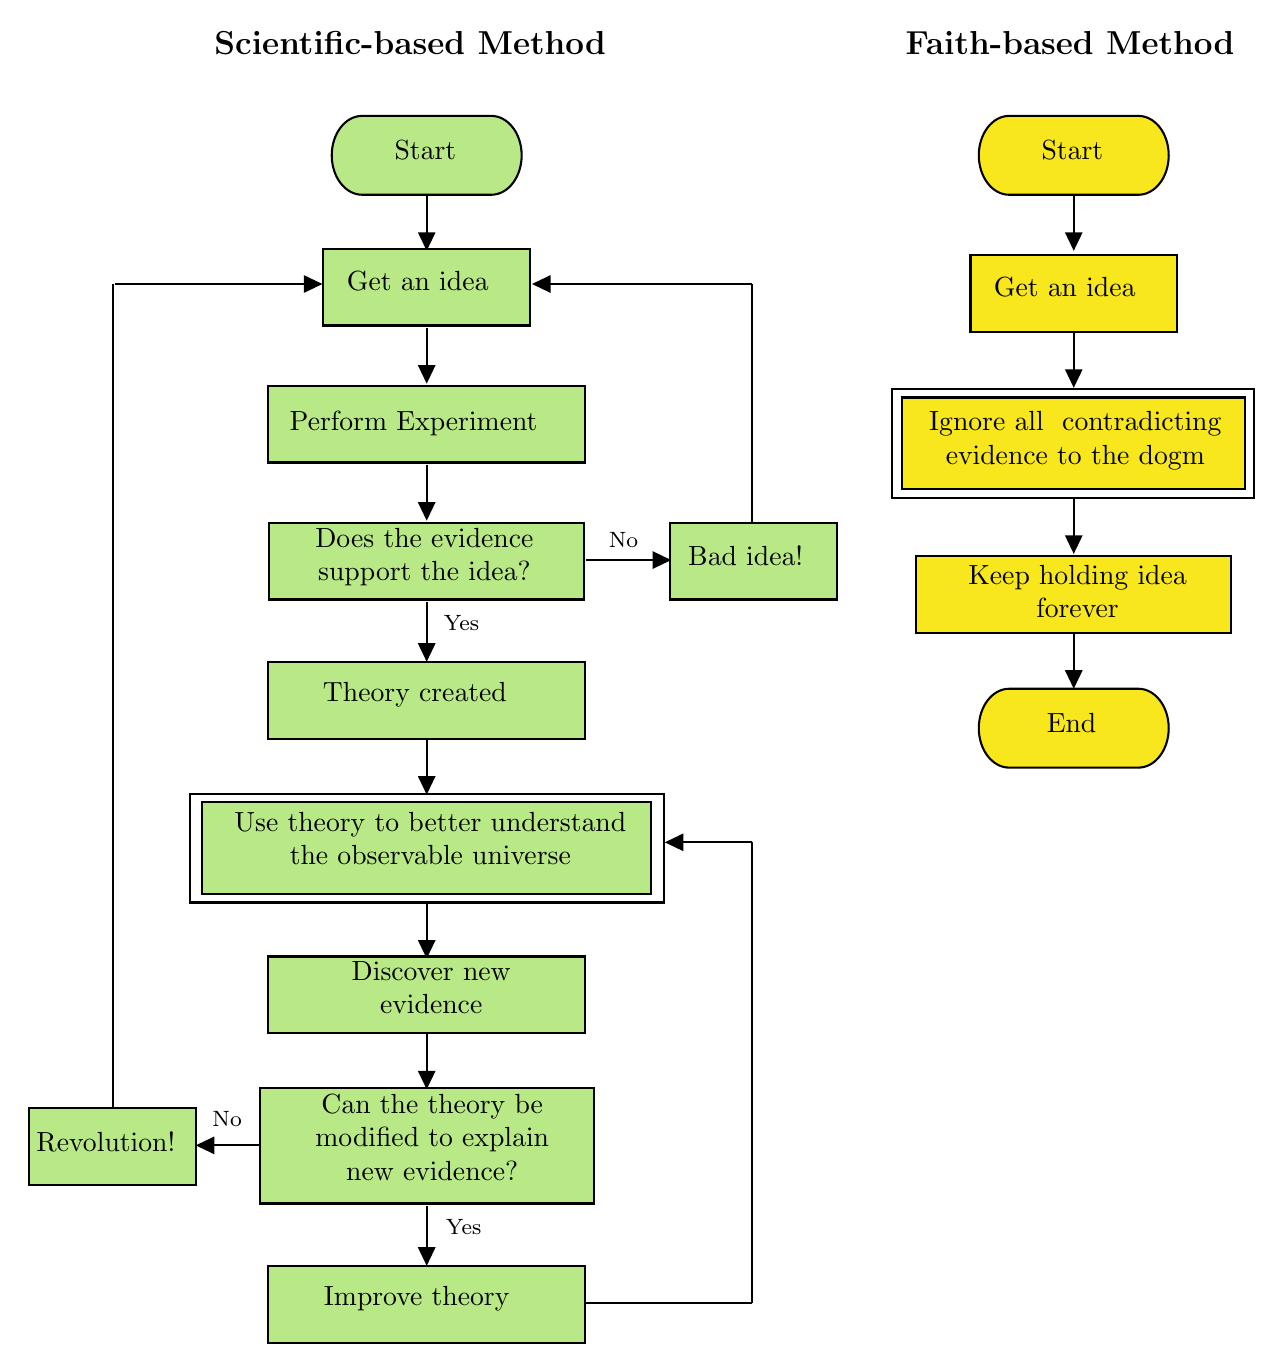
\begin{tikzpicture}[x=0.75pt,y=0.75pt,yscale=-1,xscale=1]
		%uncomment if require: \path (0,1467); %set diagram left start at 0, and has height of 1467
		
		%Shape: Rectangle [id:dp22834029140793155] 
		\draw  [fill={rgb, 255:red, 255; green, 255; blue, 255 }  ,fill opacity=1 ] (90.5,466.5) -- (319,466.5) -- (319,519) -- (90.5,519) -- cycle ;
		%Flowchart: Terminator [id:dp36967482040091304] 
		\draw  [fill={rgb, 255:red, 184; green, 233; blue, 134 }  ,fill opacity=1 ] (173.64,140) -- (235.86,140) .. controls (243.95,140) and (250.5,148.51) .. (250.5,159) .. controls (250.5,169.49) and (243.95,178) .. (235.86,178) -- (173.64,178) .. controls (165.55,178) and (159,169.49) .. (159,159) .. controls (159,148.51) and (165.55,140) .. (173.64,140) -- cycle ;
		%Straight Lines [id:da061909712056227084] 
		\draw    (204.75,178) -- (204.75,202) ;
		\draw [shift={(204.75,205)}, rotate = 270] [fill={rgb, 255:red, 0; green, 0; blue, 0 }  ][line width=0.08]  [draw opacity=0] (8.93,-4.29) -- (0,0) -- (8.93,4.29) -- cycle    ;
		%Shape: Rectangle [id:dp17947130857218463] 
		\draw  [fill={rgb, 255:red, 184; green, 233; blue, 134 }  ,fill opacity=1 ] (155,204) -- (254.5,204) -- (254.5,241) -- (155,241) -- cycle ;
		%Straight Lines [id:da33787138064232636] 
		\draw    (204.75,242) -- (204.75,266) ;
		\draw [shift={(204.75,269)}, rotate = 270] [fill={rgb, 255:red, 0; green, 0; blue, 0 }  ][line width=0.08]  [draw opacity=0] (8.93,-4.29) -- (0,0) -- (8.93,4.29) -- cycle    ;
		%Shape: Rectangle [id:dp9930647183535843] 
		\draw  [fill={rgb, 255:red, 184; green, 233; blue, 134 }  ,fill opacity=1 ] (128.5,270) -- (281,270) -- (281,307) -- (128.5,307) -- cycle ;
		%Straight Lines [id:da15263788205769946] 
		\draw    (204.75,308) -- (204.75,332) ;
		\draw [shift={(204.75,335)}, rotate = 270] [fill={rgb, 255:red, 0; green, 0; blue, 0 }  ][line width=0.08]  [draw opacity=0] (8.93,-4.29) -- (0,0) -- (8.93,4.29) -- cycle    ;
		%Shape: Rectangle [id:dp5584682841226913] 
		\draw  [fill={rgb, 255:red, 184; green, 233; blue, 134 }  ,fill opacity=1 ] (128.88,336) -- (280.63,336) -- (280.63,373) -- (128.88,373) -- cycle ;
		%Straight Lines [id:da7848044290749017] 
		\draw    (281.5,354) -- (319.5,354) ;
		\draw [shift={(322.5,354)}, rotate = 180] [fill={rgb, 255:red, 0; green, 0; blue, 0 }  ][line width=0.08]  [draw opacity=0] (8.93,-4.29) -- (0,0) -- (8.93,4.29) -- cycle    ;
		%Shape: Rectangle [id:dp468450470771381] 
		\draw  [fill={rgb, 255:red, 184; green, 233; blue, 134 }  ,fill opacity=1 ] (322,336) -- (402.5,336) -- (402.5,373) -- (322,373) -- cycle ;
		%Straight Lines [id:da73090727239734] 
		\draw    (361.5,336) -- (361.5,221) ;
		%Straight Lines [id:da5872677184303834] 
		\draw    (361.5,221) -- (258.5,221) ;
		\draw [shift={(255.5,221)}, rotate = 360] [fill={rgb, 255:red, 0; green, 0; blue, 0 }  ][line width=0.08]  [draw opacity=0] (8.93,-4.29) -- (0,0) -- (8.93,4.29) -- cycle    ;
		%Straight Lines [id:da494816536585186] 
		\draw    (204.75,374) -- (204.75,400) ;
		\draw [shift={(204.75,403)}, rotate = 270] [fill={rgb, 255:red, 0; green, 0; blue, 0 }  ][line width=0.08]  [draw opacity=0] (8.93,-4.29) -- (0,0) -- (8.93,4.29) -- cycle    ;
		%Shape: Rectangle [id:dp3969077729615893] 
		\draw  [fill={rgb, 255:red, 184; green, 233; blue, 134 }  ,fill opacity=1 ] (128.5,403) -- (281,403) -- (281,440) -- (128.5,440) -- cycle ;
		%Straight Lines [id:da474226144349555] 
		\draw    (204.75,440) -- (204.75,464) ;
		\draw [shift={(204.75,467)}, rotate = 270] [fill={rgb, 255:red, 0; green, 0; blue, 0 }  ][line width=0.08]  [draw opacity=0] (8.93,-4.29) -- (0,0) -- (8.93,4.29) -- cycle    ;
		%Shape: Rectangle [id:dp7431347056094351] 
		\draw  [fill={rgb, 255:red, 184; green, 233; blue, 134 }  ,fill opacity=1 ] (96.53,470.68) -- (312.97,470.68) -- (312.97,514.82) -- (96.53,514.82) -- cycle ;
		%Straight Lines [id:da7369308499252682] 
		\draw    (204.75,519) -- (204.75,543) ;
		\draw [shift={(204.75,546)}, rotate = 270] [fill={rgb, 255:red, 0; green, 0; blue, 0 }  ][line width=0.08]  [draw opacity=0] (8.93,-4.29) -- (0,0) -- (8.93,4.29) -- cycle    ;
		%Shape: Rectangle [id:dp2617904668241675] 
		\draw  [fill={rgb, 255:red, 184; green, 233; blue, 134 }  ,fill opacity=1 ] (128.5,545) -- (281,545) -- (281,582) -- (128.5,582) -- cycle ;
		%Straight Lines [id:da5078028185581007] 
		\draw    (204.75,582) -- (204.75,606) ;
		\draw [shift={(204.75,609)}, rotate = 270] [fill={rgb, 255:red, 0; green, 0; blue, 0 }  ][line width=0.08]  [draw opacity=0] (8.93,-4.29) -- (0,0) -- (8.93,4.29) -- cycle    ;
		%Shape: Rectangle [id:dp19329244463313544] 
		\draw  [fill={rgb, 255:red, 184; green, 233; blue, 134 }  ,fill opacity=1 ] (124.25,608.5) -- (285.25,608.5) -- (285.25,664) -- (124.25,664) -- cycle ;
		%Straight Lines [id:da22985386749875958] 
		\draw    (124.5,636) -- (96.5,636) ;
		\draw [shift={(93.5,636)}, rotate = 360] [fill={rgb, 255:red, 0; green, 0; blue, 0 }  ][line width=0.08]  [draw opacity=0] (8.93,-4.29) -- (0,0) -- (8.93,4.29) -- cycle    ;
		%Straight Lines [id:da8449301872577344] 
		\draw    (53.5,221) -- (53.5,618) ;
		%Straight Lines [id:da19812363480461292] 
		\draw    (151.5,221) -- (54.5,221) ;
		\draw [shift={(154.5,221)}, rotate = 180] [fill={rgb, 255:red, 0; green, 0; blue, 0 }  ][line width=0.08]  [draw opacity=0] (8.93,-4.29) -- (0,0) -- (8.93,4.29) -- cycle    ;
		%Shape: Rectangle [id:dp29987213666765755] 
		\draw  [fill={rgb, 255:red, 184; green, 233; blue, 134 }  ,fill opacity=1 ] (13,618) -- (93.5,618) -- (93.5,655) -- (13,655) -- cycle ;
		%Straight Lines [id:da4390453267160721] 
		\draw    (204.75,665) -- (204.75,691) ;
		\draw [shift={(204.75,694)}, rotate = 270] [fill={rgb, 255:red, 0; green, 0; blue, 0 }  ][line width=0.08]  [draw opacity=0] (8.93,-4.29) -- (0,0) -- (8.93,4.29) -- cycle    ;
		%Shape: Rectangle [id:dp0209028197709058] 
		\draw  [fill={rgb, 255:red, 184; green, 233; blue, 134 }  ,fill opacity=1 ] (128.5,694) -- (281,694) -- (281,731) -- (128.5,731) -- cycle ;
		%Straight Lines [id:da8540462766954133] 
		\draw    (281.5,712) -- (361.5,712) ;
		%Straight Lines [id:da6256129291298638] 
		\draw    (361.5,712) -- (361.5,490) ;
		%Straight Lines [id:da1686498007081123] 
		\draw    (361.5,490) -- (322.5,490) ;
		\draw [shift={(319.5,490)}, rotate = 360] [fill={rgb, 255:red, 0; green, 0; blue, 0 }  ][line width=0.08]  [draw opacity=0] (8.93,-4.29) -- (0,0) -- (8.93,4.29) -- cycle    ;
		%Flowchart: Terminator [id:dp23770588891009536] 
		\draw  [fill={rgb, 255:red, 248; green, 231; blue, 28 }  ,fill opacity=1 ] (485.39,140) -- (547.61,140) .. controls (555.7,140) and (562.25,148.51) .. (562.25,159) .. controls (562.25,169.49) and (555.7,178) .. (547.61,178) -- (485.39,178) .. controls (477.3,178) and (470.75,169.49) .. (470.75,159) .. controls (470.75,148.51) and (477.3,140) .. (485.39,140) -- cycle ;
		%Straight Lines [id:da7431657816247894] 
		\draw    (516.5,178) -- (516.5,202) ;
		\draw [shift={(516.5,205)}, rotate = 270] [fill={rgb, 255:red, 0; green, 0; blue, 0 }  ][line width=0.08]  [draw opacity=0] (8.93,-4.29) -- (0,0) -- (8.93,4.29) -- cycle    ;
		%Shape: Rectangle [id:dp2355583416446967] 
		\draw  [fill={rgb, 255:red, 248; green, 231; blue, 28 }  ,fill opacity=1 ] (466.75,207) -- (566.25,207) -- (566.25,244) -- (466.75,244) -- cycle ;
		%Straight Lines [id:da3045709994783299] 
		\draw    (516.5,244) -- (516.5,268) ;
		\draw [shift={(516.5,271)}, rotate = 270] [fill={rgb, 255:red, 0; green, 0; blue, 0 }  ][line width=0.08]  [draw opacity=0] (8.93,-4.29) -- (0,0) -- (8.93,4.29) -- cycle    ;
		%Shape: Rectangle [id:dp2656924657794639] 
		\draw  [fill={rgb, 255:red, 255; green, 255; blue, 255 }  ,fill opacity=1 ] (429,271.5) -- (603.5,271.5) -- (603.5,324) -- (429,324) -- cycle ;
		%Shape: Rectangle [id:dp7117979458993575] 
		\draw  [fill={rgb, 255:red, 248; green, 231; blue, 28 }  ,fill opacity=1 ] (433.61,275.68) -- (598.89,275.68) -- (598.89,319.82) -- (433.61,319.82) -- cycle ;
		%Straight Lines [id:da8687814174681341] 
		\draw    (516.5,324) -- (516.5,348) ;
		\draw [shift={(516.5,351)}, rotate = 270] [fill={rgb, 255:red, 0; green, 0; blue, 0 }  ][line width=0.08]  [draw opacity=0] (8.93,-4.29) -- (0,0) -- (8.93,4.29) -- cycle    ;
		%Shape: Rectangle [id:dp9684098852681449] 
		\draw  [fill={rgb, 255:red, 248; green, 231; blue, 28 }  ,fill opacity=1 ] (440.63,352) -- (592.38,352) -- (592.38,389) -- (440.63,389) -- cycle ;
		%Straight Lines [id:da2367524330588986] 
		\draw    (516.5,389) -- (516.5,413) ;
		\draw [shift={(516.5,416)}, rotate = 270] [fill={rgb, 255:red, 0; green, 0; blue, 0 }  ][line width=0.08]  [draw opacity=0] (8.93,-4.29) -- (0,0) -- (8.93,4.29) -- cycle    ;
		%Flowchart: Terminator [id:dp39220307655965847] 
		\draw  [fill={rgb, 255:red, 248; green, 231; blue, 28 }  ,fill opacity=1 ] (485.39,416) -- (547.61,416) .. controls (555.7,416) and (562.25,424.51) .. (562.25,435) .. controls (562.25,445.49) and (555.7,454) .. (547.61,454) -- (485.39,454) .. controls (477.3,454) and (470.75,445.49) .. (470.75,435) .. controls (470.75,424.51) and (477.3,416) .. (485.39,416) -- cycle ;
		
		% Text Node
		\draw (101,98) node [anchor=north west][inner sep=0.75pt]  [font=\large] [align=left] {\textbf{Scientific-based Method}};
		% Text Node
		\draw (434,98) node [anchor=north west][inner sep=0.75pt]  [font=\large] [align=left] {\textbf{Faith-based Method}};
		% Text Node
		\draw (187.75,150.5) node [anchor=north west][inner sep=0.75pt]   [align=left] {Start};
		% Text Node
		\draw (164.75,213.5) node [anchor=north west][inner sep=0.75pt]   [align=left] {Get an idea};
		% Text Node
		\draw (137.25,281) node [anchor=north west][inner sep=0.75pt]   [align=left] {Perform Experiment};
		% Text Node
		\draw (144,337) node [anchor=north west][inner sep=0.75pt]   [align=left] {\begin{minipage}[lt]{87.21pt}\setlength\topsep{0pt}
		\begin{center}
		Does the evidence\\support the idea?
		\end{center}
		
		\end{minipage}};
		% Text Node
		\draw (291,339) node [anchor=north west][inner sep=0.75pt]  [font=\footnotesize] [align=left] {No};
		% Text Node
		\draw (329.25,346) node [anchor=north west][inner sep=0.75pt]   [align=left] {Bad idea!};
		% Text Node
		\draw (211.5,379) node [anchor=north west][inner sep=0.75pt]  [font=\footnotesize] [align=left] {Yes};
		% Text Node
		\draw (153.25,411.5) node [anchor=north west][inner sep=0.75pt]   [align=left] {Theory created};
		% Text Node
		\draw (101,474) node [anchor=north west][inner sep=0.75pt]   [align=left] {\begin{minipage}[lt]{156pt}\setlength\topsep{0pt}
		\begin{center}
		Use theory to better understand\\the observable universe
		\end{center}
		
		\end{minipage}};
		% Text Node
		\draw (158.75,546) node [anchor=north west][inner sep=0.75pt]   [align=left] {\begin{minipage}[lt]{70pt}\setlength\topsep{0pt}
		\begin{center}
		Discover new\\evidence
		\end{center}
		
		\end{minipage}};
		% Text Node
		\draw (141.25,610) node [anchor=north west][inner sep=0.75pt]   [align=left] {\begin{minipage}[lt]{97pt}\setlength\topsep{0pt}
		\begin{center}
		Can the theory be\\modified to explain\\new evidence?
		\end{center}
		
		\end{minipage}};
		% Text Node
		\draw (100,618) node [anchor=north west][inner sep=0.75pt]  [font=\footnotesize] [align=left] {No};
		% Text Node
		\draw (15.25,628) node [anchor=north west][inner sep=0.75pt]   [align=left] {Revolution!};
		% Text Node
		\draw (212.5,670) node [anchor=north west][inner sep=0.75pt]  [font=\footnotesize] [align=left] {Yes};
		% Text Node
		\draw (153.75,702.5) node [anchor=north west][inner sep=0.75pt]   [align=left] {Improve theory};
		% Text Node
		\draw (499.5,150.5) node [anchor=north west][inner sep=0.75pt]   [align=left] {Start};
		% Text Node
		\draw (476.5,216.5) node [anchor=north west][inner sep=0.75pt]   [align=left] {Get an idea};
		% Text Node
		\draw (435.75,281) node [anchor=north west][inner sep=0.75pt]   [align=left] {\begin{minipage}[lt]{120pt}\setlength\topsep{0pt}
		\begin{center}
		Ignore all \ contradicting \\evidence to the dogm
		\end{center}
		
		\end{minipage}};
		% Text Node
		\draw (453.5,355) node [anchor=north west][inner sep=0.75pt]   [align=left] {\begin{minipage}[lt]{95pt}\setlength\topsep{0pt}
		\begin{center}
		Keep holding idea\\forever
		\end{center}
		
		\end{minipage}};
		% Text Node
		\draw (502,426.5) node [anchor=north west][inner sep=0.75pt]   [align=left] {End};
		\end{tikzpicture}}
	\end{center}
	
	This is important because every one of the endless series of pseudo-proofs of the existence of various gods that has been proposed, from antiquity to the present day, is automatically a failure because, as already mentioned, a logical deduction tells us nothing that is not already embedded in its premises. All logic can do for us is test the self-consistency of those premises. There is only one reliable way that humans have discovered so far to obtain knowledge they do not already possess: observation! And science is the methodical collecting of observations and the building and testing of models to describe those observations. Without falsification science would be an anarchy of logically consistent but still useless models that simply suit someone's fancy!
	
	\begin{fquote}Religion is the practice of using nonsense, in order to explain ignorance.
 	\end{fquote}
	
	Furthermore, religion has had thousands of years to provide evidence that any god exist. Yet can theists manage no better than: «\textit{YOU JUST WAIT UNTIL YOU'RE DEAD}». That tells a lot... all the more because if gods were real they wouldn't need people to argue their existence! And if theists really value faith over science then they can prove it easily: the next time they get sick they can go to a church instead of going to the hospital!
	
	\begin{fquote}A scientist will read dozens of books in his lifetime, but still known that he has a lot more to learn. A religious fanatic barely reads one book, and think that they know it all.
 	\end{fquote}
 	
 	\begin{figure}[H]
		\centering
		\includegraphics[width=0.5\textwidth]{img/intro/gods_did_it.jpg}
	\end{figure} 

	The reader must also know that at the opposite of a common myth by scientifically illiterate people, any phenomenon or assumption (even supernatural!) if well defined can be tested by the scientific method. That's why we have (among many others) scientific evidence that prayers don't provide any therapeutic effect better than a placebo. See for example about supernatural stuff the following paper \textit{Study of the Therapeutic Effects of Intercessory Prayer (STEP) in cardiac bypass patients: a multicenter randomized trial of uncertainty and certainty of receiving intercessory prayer} \cite{benson2006study} for a quite good scientific protocol and analysis or the following paper \textit{Positive therapeutic effects of intercessory prayer in a coronary care unit population} \cite{byrd1988positive} for a typical bad scientific protocol and analysis. There exist also a few meta-analysis on this supernatural topic...
	
	\begin{fquote}It doesn't matter if a great scientist was religious. What matters is that none of them ever proved their god exists!
 	\end{fquote}
 	
 	
 	\begin{figure}[H]
		\centering
		\includegraphics[width=1.0\textwidth]{img/intro/timeline_religions.jpg}
		\caption[Evolutionary tree of religions]{Evolutionary tree of religions (author: Simon E. Davies)}
	\end{figure} 
	Facts enrages believers, who prompts them to solipsism. Their only way to defend beliefs that are not concordant with scientific data is to challenge reality itself (that's why before debating with such people scientists have to agree with them about a definition of "reality" otherwise any debate is pointless)! So every time you argue with believers, because they can't address the facts they will attack the epistemology. As it is as if their position is so weak that their gods couldn't be real unless reality isn't...
	
	\begin{center}
		\includegraphics[scale=0.5]{img/intro/see_hear_spout.jpg}
	\end{center}	
	
	\pagebreak
	\subsection{Baloney detection kit}
	Through their training, scientists are equipped with what Carl Sagan name the "\NewTerm{baloney detection kit}\index{baloney detection kit}" or "\NewTerm{bullshit detection kit}\index{bullshit detection kit}" that is a set of cognitive tools and techniques that fortify the mind against penetration by falsehoods and to draw boundaries between science and pseudoscience. It isn't merely a tool of science, it contains invaluable tools of healthy scepticism that apply just as elegantly, and just as necessarily, to everyday life. By adopting the kit, we can all shield ourselves against clueless guile and deliberate manipulation. 

	There are many version of these detection tool but here is a quite complete one (but still incomplete by construction) a proposed by Michael Shermer (founding publisher of \href{http://www.skeptic.com}{Skeptic Magazine} and author of \textit{The Borderlands of Science}):
	
	\begin{enumerate}[label=\protect\circledbullet{\arabic*},leftmargin=15mm]
		\item \textit{\textbf{How reliable is the source of the claim?}}

		Pseudo-scientists often appear quite reliable, but when examined closely, the facts and figures they cite are distorted, taken out of context or occasionally even fabricated. Of course, everyone makes some mistakes. And as historian of science Daniel Kevles showed so effectively in his book The Baltimore Affair, it can be hard to detect a fraudulent signal within the background noise of sloppiness that is a normal part of the scientific process. The question is, Do the data and interpretations show signs of intentional distortion? When an independent committee established to investigate potential fraud scrutinized a set of research notes in Nobel laureate David Baltimore's laboratory, it revealed a surprising number of mistakes. Baltimore was exonerated because his lab's mistakes were random and nondirectional... So in science, there are no authorities and therefore claims are also not proofs (believing in something does not make it true!!!). At most, there are experts!

		\item \textit{\textbf{Does this source often make similar claims?}}

		Pseudo-scientists have a habit of going well beyond the facts. Flood geologists (creationists who believe that Noah's flood can account for many of the Earth's geologic formations) consistently make outrageous claims that bear no relation to geological science. Of course, some great thinkers do frequently go beyond the data in their creative speculations. Thomas Gold of Cornell University is notorious for his radical ideas, but he has been right often enough that other scientists listen to what he has to say. Gold proposes, for example, that oil is not a fossil fuel at all but the by-product of a deep, hot biosphere (micro-organisms living at unexpected depths within the crust). Hardly any Earth scientists with whom I have spoken think Gold is right, yet they do not consider him a crank. Watch out for a pattern of fringe thinking that consistently ignores or distorts data.

		\item \textit{\textbf{Have the claims been verified by another source?}}

		Typically pseudo-scientists make statements that are unverified or verified only by a source within their own belief circle. We must ask, Who is checking the claims, and even who is checking the checkers? The biggest problem with the cold fusion debacle, for instance, was not that Stanley Pons and Martin Fleischman were wrong. It was that they announced their  spectacular discovery at a press conference before other laboratories verified it. Worse, when cold fusion was not replicated, they continued to cling to their claim. Outside verification is crucial to good science.

		\item \textit{\textbf{How does the claim fit with what we know about how the world works?}}

		An extraordinary claim must be placed into a larger context to see how it fits. When people claim that the Egyptian pyramids and the Sphinx were built more than 10,000 years ago by an unknown, advanced race, they are not presenting any context for that earlier civilization. Where are the rest of the artefacts of those people? Where are their works of art, their weapons, their clothing, their tools, their trash? Archaeology simply does not operate this way.

		\item \textit{\textbf{Has anyone gone out of the way to disprove the claim, or has only supportive evidence been sought?}}

		This is the "confirmation bias" (we will come back on cognitive biases in the section of Decision Theory page \pageref{cognitive bias}), or the tendency to seek confirmatory evidence and to reject or ignore disconfirmatory evidence. The confirmation bias is powerful, pervasive and almost impossible for any of us to avoid. It is why the methods of science that emphasize checking and rechecking, verification and replication, and especially attempts to falsify a claim, are so critical. 

		\item \textit{\textbf{Does the preponderance of evidence point to the claimant's conclusion or to a  different one?}}

		The theory of evolution, for example, is "proved" through a convergence of evidence from a number of independent lines of inquiry. No one fossil, no one piece of biological or palaeontological evidence has "evolution" written on it; instead tens of thousands of evidentiary bits add up to a story of the evolution of life. Creationists conveniently ignore this confluence, focusing instead on trivial anomalies or currently unexplained phenomena in the history of life.

		\item \textit{\textbf{Is the claimant employing the accepted rules of reason and tools of research, or have these been abandoned in favour of others that lead to the desired conclusion?}} 

		A clear distinction can be made between SETI (Search for Extraterrestrial Intelligence) scientists and UFOlogists. SETI scientists begin with the null hypothesis that ETIs do not exist and that they must provide concrete evidence before making the extraordinary claim that we are not alone in the universe. UFOlogists begin with the positive hypothesis that ETIs exist and have visited us, then employ questionable research techniques to support that belief, such as hypnotic regression (revelations of abduction experiences), anecdotal reasoning (countless stories of UFO sightings), conspiratorial thinking (governmental cover-ups of alien encounters), low-quality visual evidence (blurry photographs and grainy videos), and anomalistic thinking (atmospheric anomalies and visual misperceptions by eyewitnesses).

		\item \textit{\textbf{Is the claimant providing an explanation for the observed phenomena or merely 
             denying the existing explanation?}}
	
		This is a classic debate strategy-criticize your opponent and never affirm what you believe to avoid criticism. It is next to impossible to get creationists to offer an explanation for life (other than "God did it"). Intelligent Design (ID) creationists have done no better, picking away at weaknesses in scientific explanations for difficult problems and offering in their stead. "ID did it." This stratagem is unacceptable in science.

		\item \textit{\textbf{If the claimant proffers a new explanation, does it account for as many phenomena as the old explanation did?}}
	
		Many HIV/AIDS sceptics argue that lifestyle causes AIDS. Yet their alternative theory does not explain nearly as much of the data as the HIV theory does. To make their argument, they must ignore the diverse evidence in support of HIV as the causal vector in AIDS while ignoring the significant correlation between the rise in AIDS among haemophiliacs shortly after HIV was inadvertently introduced into the blood supply.

		\item \textit{\textbf{Do the claimant's personal beliefs and biases drive the conclusions, or vice versa?}}

		All scientists hold social, political and ideological beliefs that could potentially slant their interpretations of the data (this is a "confirmation bias" also named "cherry picking" that is also by non-scientists the main cause of rejecting science results and tools), but how do those biases and beliefs affect their research in practice? Usually during the peer-review system, such biases and beliefs are rooted out, or the paper or book is rejected.  
	\end{enumerate}
	
	Some humans and especially believers (not just religious believers but on any subject for which there is no experimental evidence beyond reasonable doubt) are good at what is named "concordism". The underlying idea of concordism is to interpret texts or find random analogies in Nature (obviously having zero knowledge of combinatorics and probabilities) to justify that all the inventions or discoveries of modern science have been announced in their "holy" books or created by people belonging to the same belief group as themselves hundreds or thousands of years before others. Obviously all this masked under a hazy rhetoric, analogies that make no sense (compare statistical studies with simple texts ...), no statistical methodology, omitting to quote contradictory facts or conclusions, and with a total absence of cross-referencing sources and peer review! This obscurantism at its finest!!!

	It must be noted that this concordist approach is the prerogative of people with little education or indoctrinated since childhood (plus those suffering from mental disorders for various reasons) who are not able to identify their own biases, who are closed to any contradiction, and who are not capable of identifying the real complexity (multifactoriality) and the nuances of even a simple subject (they tend to binarize everything in True/False).
	
	\begin{fquote}You can beat 100,000 scholars with one fact, but you will very likely never beat an idiot even with 100 facts.
 	\end{fquote}
	
	\begin{figure}[H]
		\centering
		\includegraphics[width=1.0\textwidth]{img/intro/baloney_detection_toolkit.jpg}
	\end{figure}
	
	By fine tuning we can go more far about reasoning fallacies. Here is a more exhaustive list:
	\begin{enumerate}
		\item Ad hominem: An ad hominem argument attacks the messenger, not the message itself.

		\item Argument from authority: Argument that relies on the identity of an authority rather than the components of the argument itself.

		\item Argument from adverse consequences: Saying that because the implications of a statement being true would create negative results, it must not be true.

		\item Appeal to ignorance: If something is not known to be false, it must be true.

		\item Special pleading: Stating a universal principle, then insisting that it doesn't apply to your assertions for some reason.

		\item Begging the question/ assuming the answer: This occurs when a statement has an unproven premise. It is also named "circular reasoning" or "circular logic".

		\item Observational selection: Looking at only positive evidence while ignoring the negative and vice versa.

		\item Statistics of small numbers: Using small numbers in order to report large percentage increases.

		\item Misunderstanding of the nature of statistics: 	
Ignorance about central statistical assumptions and the definition of metrics (the confusion of correlation and causation, the sample size and hate of maths bias are well known example).

		\item Post hoc, ergo propter hoc: Basing an effect on a cause only on the basis of chronology.

		\item Excluded middle, or false dichotomy: Portraying an issue or argument as having only two options and no spectrum in between.

		\item Short-term vs. long-term: Assuming a current trend has remained constant throughout its history and will continue to do so in the future, even though no evidence suggests such an extrapolation is justified.

		\item Slippery slope, related to excluded middle: Saying something is wrong because it is next to or loosely related to something wrong.

		\item Suppressed evidence and half-truths: Drawing an unwarranted conclusion from premises that are at least in part correct.

		\item Weasel words: The usage of vague, non-specific references.
	\end{enumerate}
	
	In addition to teaching us what to do when evaluating a claim to knowledge, any good baloney detection kit must also teach us what not to do. It helps us recognize the most common and perilous fallacies of logic and rhetoric. Many good examples can be found in religion and politics, because their practitioners are so often obliged to justify two contradictory propositions.


	Finally, we would like to quote Antoine Lavoisier: «\textit{The physicist may also, in the silence of his laboratory and his cabinet, perform patriotic functions; he can thanks to his works reduce the mass of evils which afflict happiness and, had he not, contributed by the new roads that he opened to himself, only to delay of a few years, of a few days, the average life of humans, he could also aspire to the glorious title of benefactor of humanity.}»
	\begin{center}
		\includegraphics[scale=0.15]{img/humour/evidence_based.jpg}	
	\end{center}
	
	\pagebreak
	\section{Scientific communication backfire}
	\lettrine[lines=4]{\color{BrickRed}A}{nother} point that is important to highlight about science communication: Scientists have stop thinking that explain science will fix things and avoid people bias! Especially if you find yourself in a state of disbelief or evidence probably that drives you crazy as there are nowadays many conspiracy about flat Earth, vaccines, climate change, moon landing, etc. as mainstream media don't know how to communicate scientific papers correctly. For example, in 12010 (holocene calendar) a landmark study (see \cite{nyhan2010corrections}) showed that confronting people with hard evidence can backfire, making them more entrenched in their biases and misperceptions.

	The reasons are as follow and apply outside the case where people come listen to you or to other scientists in the context of a conference or seminar:
	\begin{enumerate}
		\item Most people don't want to listen about scientific method especially when they never asked you "is it true?", "is it the best method?", "is this not a bias?". If you use "your science" just to point out they are wrong about what they are saying or arguing you will just take them out of their comfort zone and make them even more hate science.
		
		\begin{figure}[H]
			\centering
			\includegraphics[scale=0.4]{img/intro/scientists_arent_arrogant.jpg}	
		\end{figure}
		
		\item Most humans are full of bias and they don't like to admit is it true as they assume the human is the top species of evolution and therefore cannot have such biases. So when you explain them they have biases, you just point out that they are not reliable. Speak about bias only if people ask you to do so.
		
		\item A significant percentage of people believe that their personal experience is more robust than the hundred of years of peer-review, tests, checks of the "scientific method" that has seems so far, if not THE best, at least the best one we know nowadays.
	\end{enumerate}
	\pagebreak
	\begin{fquote}No amount of peer-reviewed evidence will ever persuade an idiot, all the more if the latter is scientifically illiterate and doesn't master top level statistical calculations and the subtleties of the scientific method.
 	\end{fquote}
 	
	Now let us quote some paragraphs of an excellent \href{http://www.slate.com/articles/health_and_science/science/2017/04/explaining_science_won_t_fix_information_illiteracy.html}{{\color{blue} article}} of Tim Requarth as it is almost perfect:
	

	«The theory many scientists seem to swear by is technically known as the deficit model, which states that people's opinions differ from scientific consensus because they lack scientific knowledge. In 12010 (holocene calendar), Dan Kahan, a Yale psychologist, essentially proved this theory wrong. He \href{http://www.nature.com/nclimate/journal/v2/n10/full/nclimate1547.html}{{\color{blue} surveyed }} over 1,500 Americans, classifying each person's "cultural worldview" on a scale that roughly correlates with politically liberal or conservative. He then assessed each person's scientific literacy with questions such as "True or False: Electrons are smaller than atoms". Finally, he asked them about climate change. If the deficit model were correct, Kahan reasoned, then people with increased scientific literacy, regardless of worldview, should agree with scientists that climate change poses a serious risk to humanity.
  
	That's not what he found. Instead, Kahan found that increased scientific literacy actually had a small negative effect: The conservative-leaning respondents who knew the most about science thought climate change posed the least risk. Scientific literacy, it seemed, increased polarization. In a later study, Kahan added a twist: He asked respondents what climate scientists believed. Respondents who knew more about science generally, regardless of political leaning, were better able to identify the scientific consensus-in other words, the polarization disappeared. Yet, when the same people were asked for their own opinions about climate change, the polarization returned. It showed that even when people understand the scientific consensus, they may not accept it.
	
	\begin{fquote}[Average social network user]Having no postgraduate education on this subject, nor having any biases and having done no research in a lab at a professional level whatsoever, I don't understand it. Therefore, it doesn't make sense and is false!
 	\end{fquote}

	The takeaway is clear: Increasing science literacy alone won't change minds. In fact, well-meaning attempts by scientists to inform the public might even backfire. Presenting facts that conflict with an individual's worldview, it turns out, can cause people to dig in further. Psychologists, aptly, dubbed this the "backfire effect".
	\begin{figure}[H]
		\centering
		\includegraphics[scale=0.35]{img/intro/explain_science.jpg}
		\caption[]{source: \url{https://www.ratbotcomics.com}, author: Dr. Jones}
	\end{figure}
	If scientists simply want to explain science to a curious audience, disseminate their research more broadly, or write for fun, this doesn't matter much. But if scientists are motivated to change minds-and many enrolled in science communication workshops do seem to have this goal-they will be sorely disappointed.

	That's not to say scientists should return to the bench and keep their mouths shut. They should just realize that closing the "information gap" isn't the goal. And instead, they need to learn how to communicate science strategically.

	There are obvious reasons why science communication is a necessary and worthwhile endeavour, but a huge one is that there's a politically motivated push to destabilize scientific authority. At a Heartland Institute conference last month, Lamar Smith, the Republican chairman of the House science committee, told attendees he would now refer to "climate science" as "politically correct science", to loud cheers. This lumps scientists in with the nebulous "left" and, as Daniel Engber pointed out here in Slate about the upcoming March for Science, rebrands scientific authority as just another form of elitism.

	Is it any surprise, then, that lectures from scientists built on the premise that they simply know more (even if it's true) fail to convince this audience? Rather than fill the information deficit by building an arsenal of facts, scientists should instead consider how they deploy their knowledge. They may have more luck communicating if, in addition to presenting facts and figures, they appeal to emotions. This could mean not simply explaining the science of how something works but spending time on why it matters to the author and why it ought to matter to the reader. Research also shows that science communicators can be more effective after they've gained the audience's trust. With that in mind, it may be more worthwhile to figure out how to talk about science with people they already know, through, say, local and community interactions, than it is to try to publish explainers on national news sites. And they might consider writing op-eds for their local papers, focusing on why science matters to their particular communities.

	Scientists can also learn to avoid certain pitfalls. I spoke with Gretchen Goldman, research director of the Union of Concerned Scientists' Center for Science and Democracy, which offers communication and advocacy workshops. A counter-intuitive lesson she's learned is that refuting stories that deny climate change by addressing each claim and explaining why it's wrong is not that productive. In fact, it could be counter-productive: "If you repeat the myth, that's the part people remember even if you immediately debunk it", she says. A better approach, she suggests, is to reframe the issue. Don't just keep explaining why climate change is real, explain how climate change will hurt public health or the local economy. Communication that appeals to values, not just intellect, research shows, can be far more effective.

	[...] But the obstacles faced by science communicators are not epistemological but cultural. The skills required are not those of a university lecturer but a rhetorician.

	So it's an admirable goal to communicate about science, but almost certainly destined to fail. This is because the way most scientists think about science communication - that just explaining the real science better will help - is quite wrong. It's so wrong that it may have the opposite effect of what they're trying to achieve. [...]»
	
	\begin{fquote}Silence is sometimes the best answer to the fools.
 	\end{fquote}
	
	\begin{center}
		\includegraphics[scale=0.35]{img/intro/lies_vs_comfort.jpg}	
	\end{center}
	\begin{fquote}As a scientist (and atheist) you will often be hated by all those who believe in fairy tales and think that their opinions, anecdotes, circular logic and scientific illiteracy are worth it, but those who stands firm to the Scientific Method and to the precautionary principle will be saved and will help to save the haters. Comforting lies have always and are still taking the elevator and the Scientific Method takes the stairs, the lies will come first but one day or another the Science will always catch up with its unpleasant evidence.
 	\end{fquote}
	
	\pagebreak
	\section{Is Science dogmatic?}
	We will here mainly repeat things that we have already mentioned earlier above. However as some scientifically illiterate people still think in this beginning of the 121st century (holocene calendar) that YouTube videos containing some rhetorical monologue\footnote{As already said people should not trust monologues - whether on radio, television or any social network - because there are no experts to counter the possible wrong arguments or ill-defined concepts that may lead a part of the audience to wrong speculative interpretations! In addition, humans under the stress of knowing that they are recorded are naturally prone to vocabulary errors and that's without counting the more than 200 cognitive biases in the brain which sometimes lead to the erroneous simplification of complex thoughts... !} or some books without proofs and without statistical data analysis constitute some sort of "evidence" it is necessary maybe to come back on a few topics but with a different perspective\footnote{And please don't forget that the purpose of Science is not the "Truth" but it's only a tool that explains quite well things that we see or feel following the best actual models. And also please don't forget that quoting a book, a famous scientist, a blog or a YouTube video is only at best an evidence of level 2 or 3!}!
	
	For Science, if something exist with evidence beyond reasonable doubt (BRD), at its actual state of knowledge, then it means it can be measured! If it cannot be measured or is ill-defined, well, then science can't provide evidence that it doesn't exist (don't forget that the purpose of Science is to refute models and if it fails to do so a long time enough then a Model may take the status of Theory!). In a simplistic and slightly out of context metaphor, this is equivalent to say that for the blind (taking away all their other senses) the world doesn't exist with strong evidence because they cannot see it nor feel it. Some people then say that Science is materialist! However this doesn't mean at all that Science has failed as an investigation method, however it just means that Science knows it doesn't know everything otherwise it would stopped and that the scientific method must be corrected constantly according to the new available evidences.
	
	Typically Science don't reject completely parapsychology powers or the existence of one of the thousand of deities created around the World by humans even if actually all experimental tests have rejected them with strong evidence (but not definitively!). The advocates of parapsychology or religions (or of some alternative medicines) may argue that Science can't prove nor disprove what it can't measure directly or indirectly. And they are very likely absolutely right! Science can only \underline{fail to reject with a given level of evidence} if something exist or not \underline{at its actual level of knowledge}. So if someone argue that flying unicorns exist without providing a protocol so that thousands of other people can check this fact in a reproducible way... then Science (scientists) humbly say us that: «\textit{we don't have any evidence beyond reasonable doubt at our actual state of knowledge that unicorn exist or not!}»
	
	So it's not Science that is dogmatic, nor the huge majority of the scientific community. But only some bad educated and biased scientists (nobody is perfect...).
	
	\begin{figure}[H]
		\centering
		\includegraphics[width=0.9\textwidth]{img/intro/science_dogmatic.jpg}
	\end{figure}
	
	Some humans don't like that scientists may not know everything about something, or that scientists do errors, and that science takes time and that even worst, these same people will maybe never have an answer to their main questions before their death. But that's how Science works actually!!! If anyone finds a more reliable and fast way to investigate the Universe and its phenomena than the actual state of the Scientific Method, then the majority of the scientific community - especially the academic part - is waiting to check it and if it works indeed better to adopt it!
	
	\begin{fquote}[Carl Sagan]Extraordinary claims require extraordinary evidence.
 	\end{fquote}

	 So some people may ask Science to be truly scientific, meaning, it should question itself regarding the certainty of their own postulates and instruments. But as we already said many times in the previous sections above, this is what researchers do in their daily work!!! They try to find new evidence to reject actual theories, models, methods, postulates or bad instruments... otherwise Science would stop and scientists would lost their job. However the process is slow and takes days, weeks, months, years, decades, centuries and sometimes even millenniums.
	 
	\begin{tcolorbox}[enhanced,title=Remark,colframe=black,arc=10pt,drop lifted shadow,after skip=15pt plus 2pt,,breakable]
	Some people point out that the version of the Universe scientists currently have is only what their instruments, and especially their imagination allows them to understand. And they are right! We - all professional academic researchers - know that fact since centuries in Science and that's why every day we try to push the boundaries of knowledge (hence also of imagination) and to develop new instruments and methods to measure things that were not even known a few decades before! Keep in mind this is what we are paid for! If there is nothing new to discover we will all lost our jobs!\\
	
	So yes in its current state, Science cannot account for consciousness phenomena, synchronicity, or even near death experiences or spontaneous epiphanies, etc. But well educated professionals scientists won't claim they do or don't exist because we don't have yet any experimental reproducible evidence to support any of these positions! Scientists are just waiting for those who claim that such things exist - and even run quite good business with it - to provide us reproducible experimental evidence. Sadly so far all the people who made such claim and run business with them have failed to provide any evidence or were just simply debunked and that's all.\\
	
	Anyone should ask himself why evangelist pastors or any kind of miraculous healer (...) don't practice their art in the scientific controlled environment of Hospitals rather that in their church (in front of a public in the huge majority biased, uneducated and scientifically illiterate) or with a small group of unknown and suspicious people behind a camera.......
	\end{tcolorbox}
	 
	People like Rupert Sheldrake, a PhD holder (from Cambridge) in biochemistry and retired researcher in the field of parapsychology who proposed the concept of morphic resonance... and also author of numerous rewarding books...... explores ten dogmas of Science that should be reconsidered according to his personal and subjective opinion... 
	
	Let us present below these ten dogmas and... we will comment them as Dr. Sheldrake doesn't have a PhD in Physics, nor in Cosmology but has a good sense of rhetoric especially when he does a monologue in front a public of neophytes (the reader and Dr. Sheldrake will be able to find the mathematical proof of our answers in the $8,000$ pages of this book if they are curious - as at the opposite of Dr. Sheldrake we like proofs and experimental evidence more than rhetorical monologue...):
	\begin{enumerate}
		\item \og Nature is mechanic: all the creatures and systems of nature are robots made to follow a given genetic program. \fg{}
		
		$\vartriangleright$ Our comment: We are not sure of how the word "Mechanics" is defined in this sentence (the basics of a debate is to agree on the meaning of words...) but obviously a biological system cannot be compared to a mechanical one (mechanical system doesn't evolve). However as we will prove it in this book Nature is Information based at all levels, Probabilistic based at the microscope level, and behaves Statistically and Mechanically at macroscopic level. So as most of the time in Science..., it's not as easy as it seems to be (it seems that Dr. Sheldrake has a binary vision of the World and of the Universe that is quite surprising given his supposed level of education).
		
		\item \og Matter is unconscious: Plants, stars, animals and elements are material things that are and cannot have a consciousness of themselves. \fg{}
		
		$\vartriangleright$ Our comment: First we should ask how is "consciousness" defined by Dr. Sheldrake. Secondly, who asserted that in the scientific community? Is there a written scientific consensus on this subject or it comes out from the imagination of Dr. Sheldrake?

		\item \og The laws of nature are fixed: At the moment of the Big Bang all the necessary constants until the end of time were established. The habits of nature do not evolve. \fg{}
		
		$\vartriangleright$ Our comment: What scientific consensus stated that? That's very likely wrong as actually we have a few mathematical-physics models that proves that the constants of the Universe may have changed and also experimental evidence that maybe the laws of Nature may have changed. But one thing is almost sure: there is no scientific consensus yet on that topic!

		\item \og The amount of nature and energy in the Universe is always the same. \fg{}
		
		$\vartriangleright$ Our comment: The scientific community has strong evidence beyond reasonable doubt of that statement for the \underline{observable} Universe. However the dynamic of the Universe disprove energy conservation at large scales (this is derived from Noether theorems!). Notice that we have however no evidence yet of this statement of energy conservation for the whole Universe (the observable and not observable one).

		\item \og Nature has no purpose: there is no design in nature in terms of intention and the process of evolution is mechanic. \fg{}
		
		$\vartriangleright$ Our comment: We have strong evidence beyond reasonable doubt indeed that there is no design as the existing design are flawed in many ways. And the process of evolution as proven mathematically in this book and experimentally (beyond any reasonable doubt) in laboratories is not mechanical but stochastic.

		\item \og Biologic Heritage: The plans to produce a living being are composed within the physical matter lodged in their genes. \fg{}
		
		$\vartriangleright$ Our comment: That's not completely correct. Experimental observations provide us that some basics of the plans are random and influenced by external and internal modifications. Again Dr. Sheldrake gives a binary view of a phenomenon which is far more complex. But this is something we know as typical of scientific illiterate people: they reduce something complex to something simple because they can't grasp the complexity of the World and of the Universe.

		\item \og Memory is kept in the brain as material prints: memory is made of proteins and nerve endings organized as a drawer within itself. \fg{}
		
		$\vartriangleright$ Our comment: If it was the case we wouldn't forget things... That's because the brain is far more complex and involves probabilities, Bayesian and stochastic process that we know why the human brain forgets things and has sometimes building issues...

		\item \og Mind is in the head: The mind has a physical connection with the head and the brain, relegating intellectual subordination on the rest of the body. \fg{}
		
		$\vartriangleright$ Our comment: What is the "Mind" for Dr. Sheldrake? As far as we know there is no scientific consensus about its definition. Furthermore is Mind what we observe in MNR scanners?

		\item \og Phenomena like telepathy are impossible: thoughts have no effect in the world because of number 8 on the list (the mind is in the head). \fg{}
		
		$\vartriangleright$ Our comment: What scientific consensus or community stated that? Actually Science has no evidence that telepathy works or exist, yes (!) - but no well educated scientist would say it is "impossible" (by the way any well educated scientist know that is better to avoid using the word "impossible" about an unknown future or unmeasurable phenomena).

		\item \og Only mechanical medicine works: It is merely by chance or placebo effects that traditional healing practices or natural remedies have any effect on people's health. \fg{}
		
		$\vartriangleright$ Our comment: Again... what scientific consensus or community stated that? That's not accurate. Maybe scientists agree on the fact that actually not other method than the Scientific Medicine has provided better odds ratio than other medicines. But if one day some people provide robust evidence that traditional healing practices or natural remedies work, then almost surely they will be promoted by the scientific academic community.
	\end{enumerate}
	
	If this is the best support Dr. Sheldrake has for his position, then this means that there is no support. It is entirely based on gish gallop and speculation, pointing to common misconceptions and popular opinions rather than evidence and examples of "dogma" in science.
	
	We can understand why someone reading or listening this kind of gish gallop may think that there is some basis of evidence. Gish gallop means making loads of claims without evidence, leaving the opposition the large job of checking each and every claim. Even so, when someone claims the "establishment" is dogmatic, immoral or whatsoever, we may sincerely hope that any reader will critically assess that person claims.
	
	\begin{fquote}[?]A religious belief without dogma is not possible and science is not compatible with any dogma. So science can only be incompatible with religious beliefs.
 	\end{fquote}
	
	\begin{figure}[H]
		\centering
		\includegraphics[width=0.7\textwidth]{img/intro/false_equivalence.jpg}
		\caption{False equivalence fallacy}
	\end{figure}
	
	\begin{flushright}
	Section quality score: \score{4}{5} 151 votes, 75.23\%
	\end{flushright}